\documentclass[../ei103948-project-documentation.tex]{subfiles}
\begin{document}
\section{Diseño}

\subsection{Diseño de la arquitectura de software}
    Nuestra arquitectura se centrará en tres características básicas principalmente, además de usar la estrategia \textit{ATTD}\footnote{\textbf{ATDD}: \textbf{A}cceptance \textbf{T}est \textbf{D}riven \textbf{D}evelopment} para su desarrollo. La primera será simplicidad; la reutilización de código y baja complejidad es clave en proyectos para la reducción de errores. La segunda será extensibilidad; queremos que sea sencillo de añadir nuevos servicios en el futuro sin cambiar toda la arquitectura. La tercera y última será configurabilidad; ya que queremos que sea fácil definir el comportamiento de estas extensiones.\\

    La aplicación utiliza una arquitectura \cite{granell-estilosarquitectura} cliente-servidor. Sin embargo, al contrario que muchos otros proyectos, estos están totalmente desacoplados. No utilizando motores de plantillas como \textbf{Thymeleaf}, ni residiendo el mismo repositorio. Esto es posible gracias a una \textit{API REST}\footnote{\textbf{REST}: \textbf{Re}presentational \textbf{S}tate \textbf{T}ransfer} que se utiliza como contratado para la comunicación. Además, debido a esto ambas partes se pueden ver como proyectos separados, los cuales tienen su propia arquitectura interna y se desarrollarán por separado.\\

    \begin{figure}[H]
        \begin{center}
        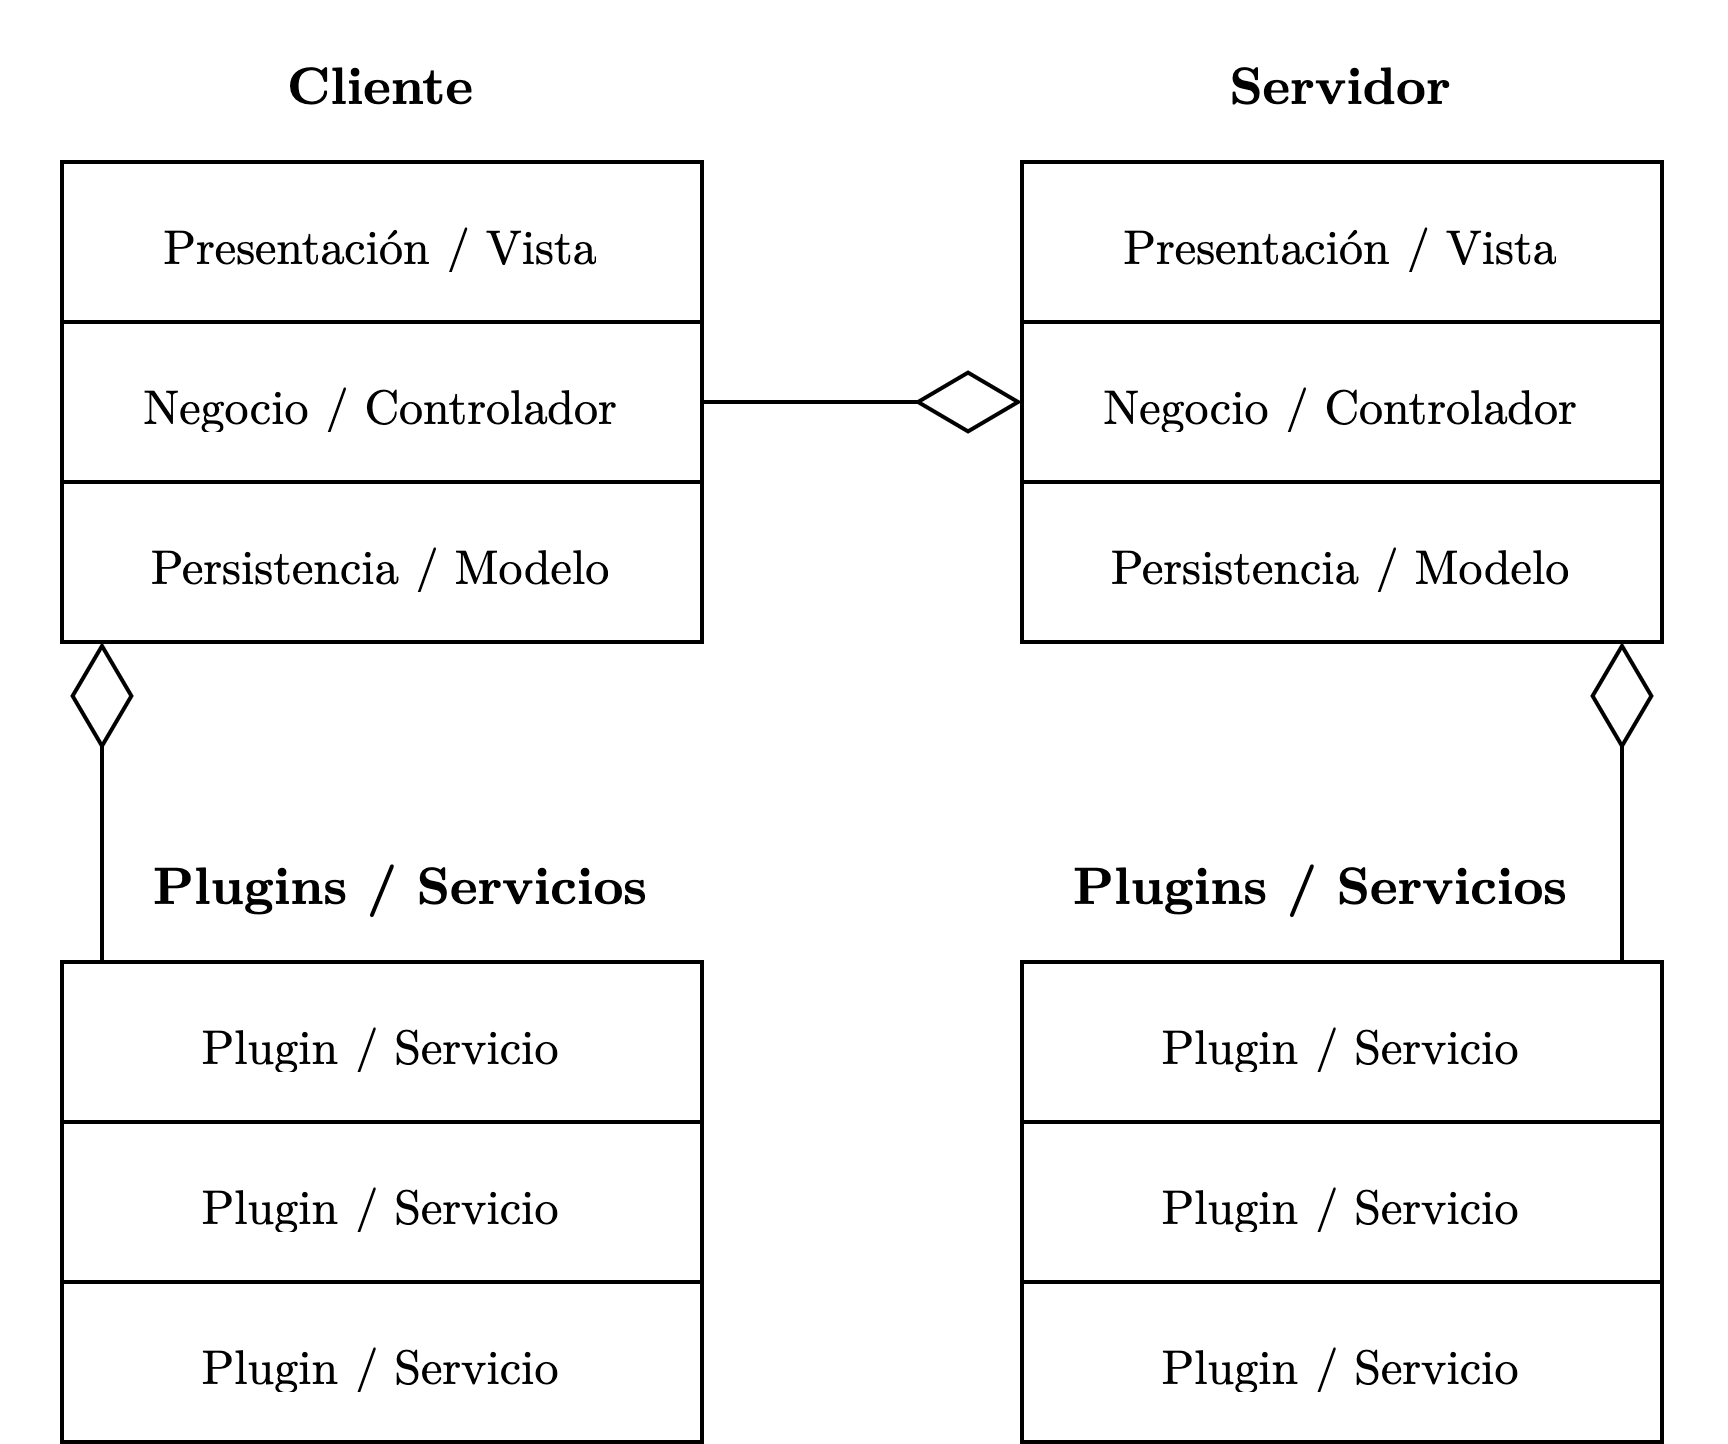
\includegraphics[scale=0.20]{images/DisenyoArquitecturaSoftware.png}
        \end{center}
        \caption{Esquema de capas de nuestra arquitectura}
    \end{figure}

    Nosotros hemos optado por, en ambas partes, una arquitectura monolítica de microkernel con un núcleo particionado; siendo la lógica principal el núcleo y los servicios ofrecidos los plugins. Esto nos permite dos cosas principalmente: al núcleo seguir una arquitectura de tres capas \textit{MVC} y a los plugins ser totalmente independientes, pudiendo añadir servicios adicionales sin tener que modificar el núcleo.\\

    La capa de presentación o vista en el caso del servidor hace referencia a los objetos Java serializados que se presentan como \textbf{JSON}s; siendo esta una vista pero para otros sistemas software. Sin embargo, la vista del cliente si corresponde a una vista tradicional, para usuarios finales.\\

    Toda esta separación podría parecer contraproducente a primera vista, sobre todo dado nuestro principio de simplicidad, sin embargo proporciona todo lo contrario. Al dividir el tanto el software lo que queda son capas de tamaño mínimo y simples, algunas pudiéndose implementar en tan solo una clase o fichero.\\

    El servidor está basado en \textbf{Java} y proporciona esta \textit{API} web que abstrae toda la lógica de negocio. Dando acceso a la gestión de datos del usuario y además todos los datos que necesite el cliente pero normalizados, como el clima o las noticias. Utilizando el patrón \textit{facade} internamente para simplificar el acceso a los diferentes servicios antes de publicarlos.\\

    El cliente está basado en \textbf{React} y proporciona un vista ligera y mínima sobre la \textit{API} en un navegador web, sin lógica alguna para el procesamiento de datos. Dando acceso a una interfaz sencilla que pueda usar cualquier tipo de usuario, similar a la de \textbf{Google Discover} en los dispositivos móviles.\\

    Las pruebas relacionadas con el paradigma \textit{ATDD} se realizan solo en el subsistema del servidor, simplificando así su implementación al excluir la interfaz gráfica. Esto igualmente no reducirá la efectividad de ellas, debido a que la superficie del cliente será mínima. Todas las pruebas integrarán todos los componentes posibles, realizando incluso llamadas \texttt{HTTP} al servidor y acceso a la base de datos del entorno de desarrollo, asegurando así una adecuada configuración de toda la pila.

    \subsection{Tecnologías utilizadas}
				\subsubsection{Dependencias y tecnologías}

				Nuestro proyecto, utiliza varias tecnologías todas interconectadas y configuradas para minimizar el tiempo de desarrollo. El proyecto intenta ser lo más sencillo posible de construir y ejecutar, basado en conceptos conocidos para no ir sin ninguna guía, pero nuevos elementos para incentivar así su desarrollo.\\

				El servidor está basado en \textbf{Java}, principalmente haciendo uso de \textbf{Spring Framework}, específicamente \textbf{Spring Boot}. Debido a nuestra formación previa, inyección de dependencias por anotaciones y conversiones a \textbf{JSON}\footnote{\textbf{JSON}: \textbf{J}ava\textbf{S}cript \textbf{O}bject \textbf{N}otation} automáticas, lo hace una opción idónea para el servicio \textit{REST} que queremos crear en el proyecto. Además, este incorpora ya de fábrica \texttt{JUnit}\footnote{\textbf{JUnit}: es un conjunto de bibliotecas utilizadas en programación para hacer pruebas unitarias de aplicaciones \texttt{Java}.} con varias modificaciones, como \textit{Runners} especiales que ejecutan servidores de prueba.\\

				También para simplificar todo del código \textit{boilerplate} que hace falta en \textbf{Java} como constructores, getters, setters, etc; usamos \textbf{Lombok}. Esta es una librería que proporciona múltiples anotaciones para generar estos métodos automáticamente. La ventaja de ello respecto a los generadores en \textit{IDE} es que este mantiene el código fuente sin modificaciones, por lo cual queda simple y minimalista.\\

				Almacenando datos de manera persistente, utilizaremos el sistema gestor de bases de datos \textbf{H2}. Este permite ejecutarlo de manera empotrada en la propia aplicación, eliminando la gestión de otro servicio externo. Además provee un modo de ejecución solo en memoria, ideal para ejecutar tests en entornos aislados. También simplificamos su uso y mantenemos el sistema gestor desacoplado usando \textbf{JPA}. Esto te permite definir el modelo de tus datos directamente en las clases y abstrae toda la generación de tablas y \textit{DAOs}. Además, se usará \textbf{Jasypt} para cifrar cualquier dato sensible, como las contraseñas de los usuarios, antes de guardarlas.\\

				Debido a que este servidor es el encargado de abstraer otras \textit{APIs REST} y que también queremos probar nuestra propia \textit{API}, hacemos uso del framework \textbf{REST Assured}. Esto hace que el acceso a \textit{APIs} y los datos que estas devuelven sean sencillos y declarativos.\\

				Dentro del apartado de las pruebas hemos complementado esta última con \textbf{Hamcrest}, ya que proporciona más utilidades declarativas para la validación de elementos, pero de carácter general similar a \textbf{JUnit}. También, hacemos uso de \textbf{Mockito}\cite{mockito2}\footnote{\textbf{Mockito}: es un marco de prueba de código abierto para \textbf{Java} lanzado bajo la Licencia \textit{MIT}}, esto simplifica la generación de \textit{Mocks} enormemente. Además de contar con una muy buena integración con \textbf{Spring} y su inyección de dependencias.\\

				Debido a que todas estas peticiones que realizamos son costosas y estas \texttt{API} imponen su propio límite, también hacemos uso de la anotación de \texttt{Cacheable} proporcionada por \textbf{JCABI Aspects}. Esto reduce el tiempo de latencia y el número de peticiones inmensamente, Todo ello sin necesitar crear métodos especialmente diseñados para ello y pudiendo especificar el tiempo máximo de memorización. Esta incluye muchas otras anotaciones útiles pero principalmente la usaremos por esa.\\			

				El cliente está basado en \textbf{React} por lo que utiliza una gestión totalmente diferente a la de \textbf{Java}. Mitigando esto hacemos uso de \textbf{Frontend Maven Plugin}, el cual permite conectar tecnologías web frontend con \textbf{Java} y \textbf{Maven} fácilmente. Este instala \textbf{Node} y un gestor de paquetes (\textbf{NPM}) a partir de un Maven goal, el cual hemos configurado para que se enlace con la acción de construcción de proyecto. Además de incorporar \textbf{Babel} como compilador \textbf{JSX} para \textbf{React}, y \textbf{Webpack} para empaquetar todas estas dependencias una vez compiladas a un único fichero.

                El proyecto está basado en la versión más reciente del \textbf{JDK}, hasta el momento \textbf{JDK} 17, pero es posible que pueda funcionar en otras versiones más antiguas. Las dependencias, tanto del lado de \textbf{Java} como \textbf{JavaScript}, también son las más recientes hasta el momento. La única excepción a esto es el plugin de \textit{frontend} para \textbf{Maven}, ya que esta requiere una versión de Maven que la mayoría de editores no tienen por defecto. Es por ello que se ha mantenido en una versión anterior, eliminando así la necesidad de instalar software adicional manualmente.

				\begin{figure}[H]
					\begin{center}
					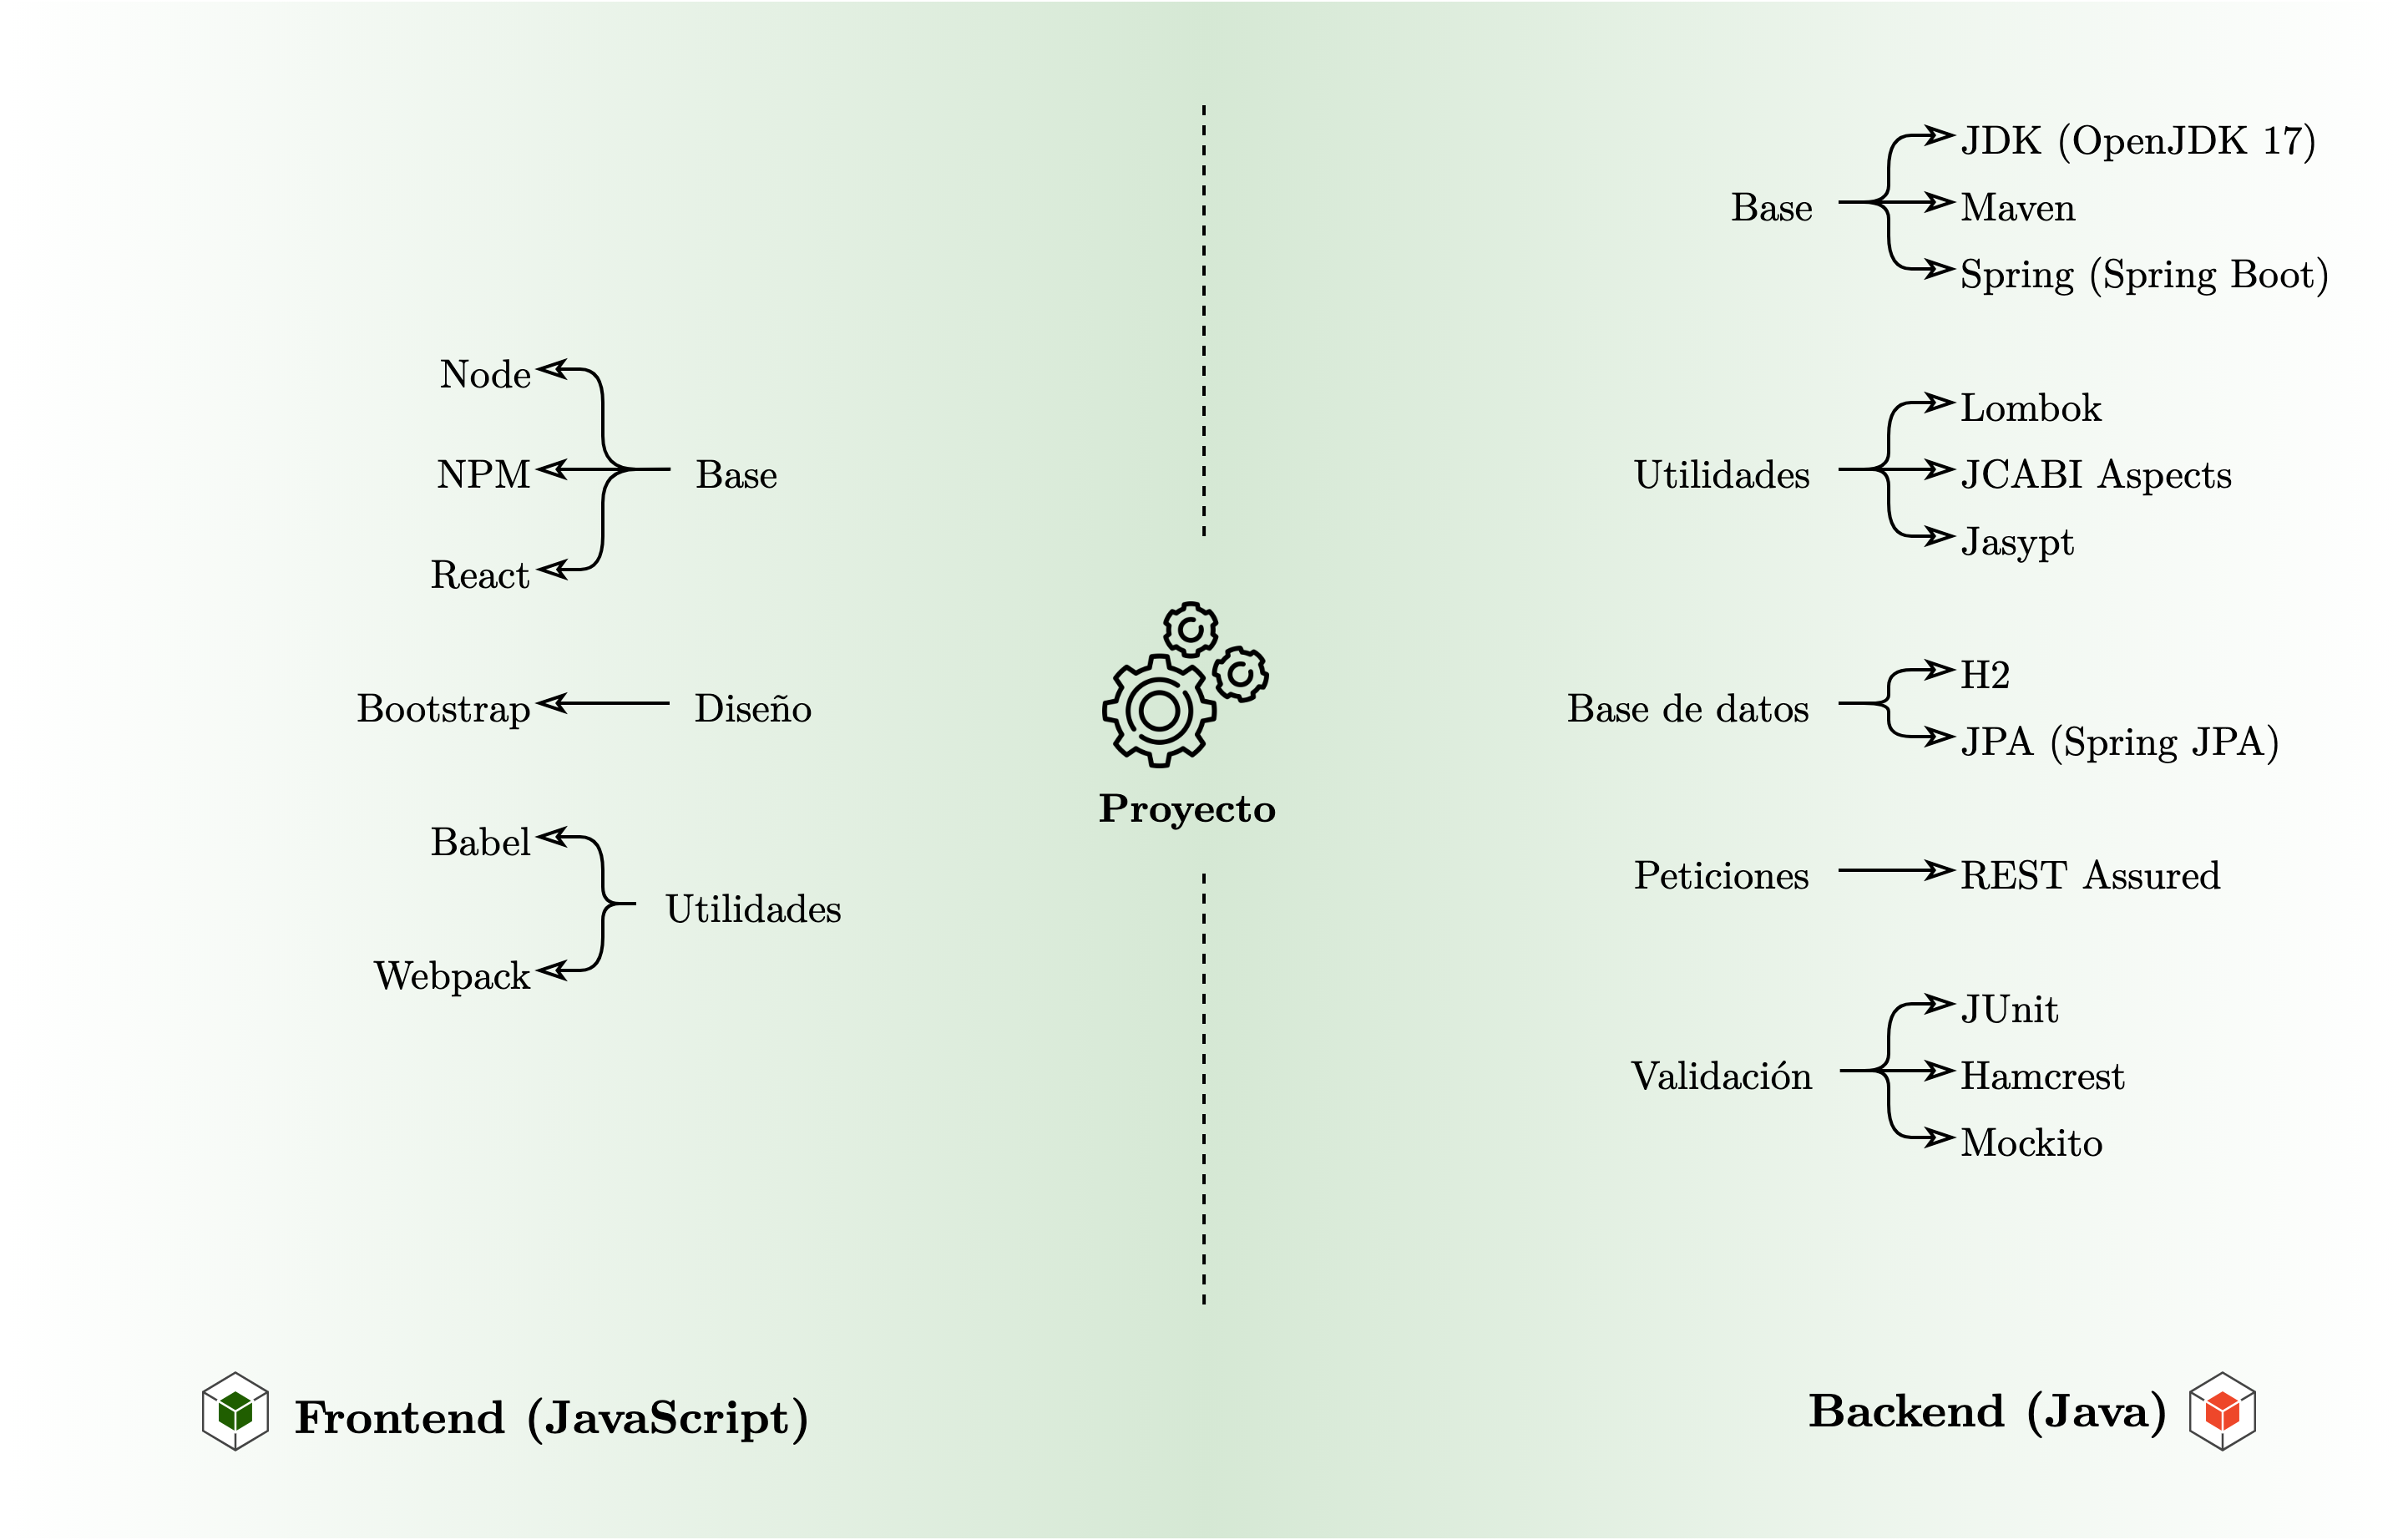
\includegraphics[scale=0.15]{images/FrontBackEnd.png}
					\end{center}
					\caption{Esquema de las tecnologías implementadas en el proyecto}
				\end{figure}

				El esquema de consulta de la documentación que hemos precisado para llevar a cabo el proyecto de forma íntegra se encuentra en la sección B (\textit{Apéndices - B.Documentación}).

                \subsection{Patrones de diseño}
    
                Diseñar software orientado a objetos no es una tarea fácil, y es aún más complicado el diseñar software orientado a objetos reutilizable. Hay que encontrar los objetos pertinentes, factorizarlos en clases con la granularidad adecuada, definir interfaces de clases y jerarquías de herencia y establecer las principales relaciones entre esas clases y objetos.\\
            
                Como una mera definición de patrón de diseño podríamos decir que: '\textit{Cada patrón describe un problema que ocurre una y otra vez en nuestro entorno, así como la solución a ese problema, de tal modo que se pueda aplicar esta solución un millón de veces, sin hacer lo mismo dos veces}'. Aunque esta vaga definición engloba todo tipo de patrones, para el campo de la prograación orientada a objetos nuestras soluciones se expresan en términos de objetos e interfaces, en vez de paredes y puertas, pero en la esencia de ambos tipos de patrones se encuentra una solución a un problema dentro de un contexto \cite{patronesdisenyo}. Por norma general, cada patrón tiene cuatro elementos esenciales:
                    \begin{enumerate}[I)]
                        \item El \textbf{nombre del patrón}.
                        \item El \textbf{problema} que describe el momento idóneo de aplicar el patrón.
                        \item La \textbf{solución}: diseño, relaciones, responsabilidades y colaboraciones.
                        \item Las \textbf{ventajas y desventajas} de utilizar dicho patrón en un problema dado.
                    \end{enumerate}
            
                Los patrones de diseño varían en su granularidad y nivel de abstracción. Dado que existen muchos patrones de diseño, es necesario un modo de organizarlos. Entre los patrones identificados e implementados, la clasificación es la siguiente (\faIcon{pencil-alt}: Implementado e \faIcon{eye}: Identificado):
                    
                    \begin{itemize}
                        \item \textbf{Creacionales}:
                            \begin{itemize}
                                \item [\faIcon{pencil-alt}] \texttt{Factory Method}.
                                \item [\faIcon{eye}] \texttt{Singleton Method}.
                            \end{itemize}
                        \item \textbf{Estructurales}:
                            \begin{itemize}
                                \item [\faIcon{pencil-alt}] \texttt{Facade}.
                                \item [\faIcon{eye}] \texttt{Proxy}.
                            \end{itemize}
                        \item \textbf{Comportamiento}:
                            \begin{itemize}
                                \item [\faIcon{pencil-alt}] \texttt{Template Method}.
                                \item [\faIcon{eye}] \texttt{Dependency Inversion}.
                            \end{itemize}
                    \end{itemize}
            
            
                En este proyecto, hablando de patrones de diseño en el software, podemos identificar algunos que están ya implementados por parte del software que hemos utilizado y otros que hemos implementado nosotros manualmente.\\
                
                A modo de resumen, a continuación un esquema con los patrones que hemos identificado, implementado y patrones relacionados (que no están implementados).
            
                \newpage
                \begin{figure}[H]
                    \begin{center}
                        \hspace*{-10mm}
                    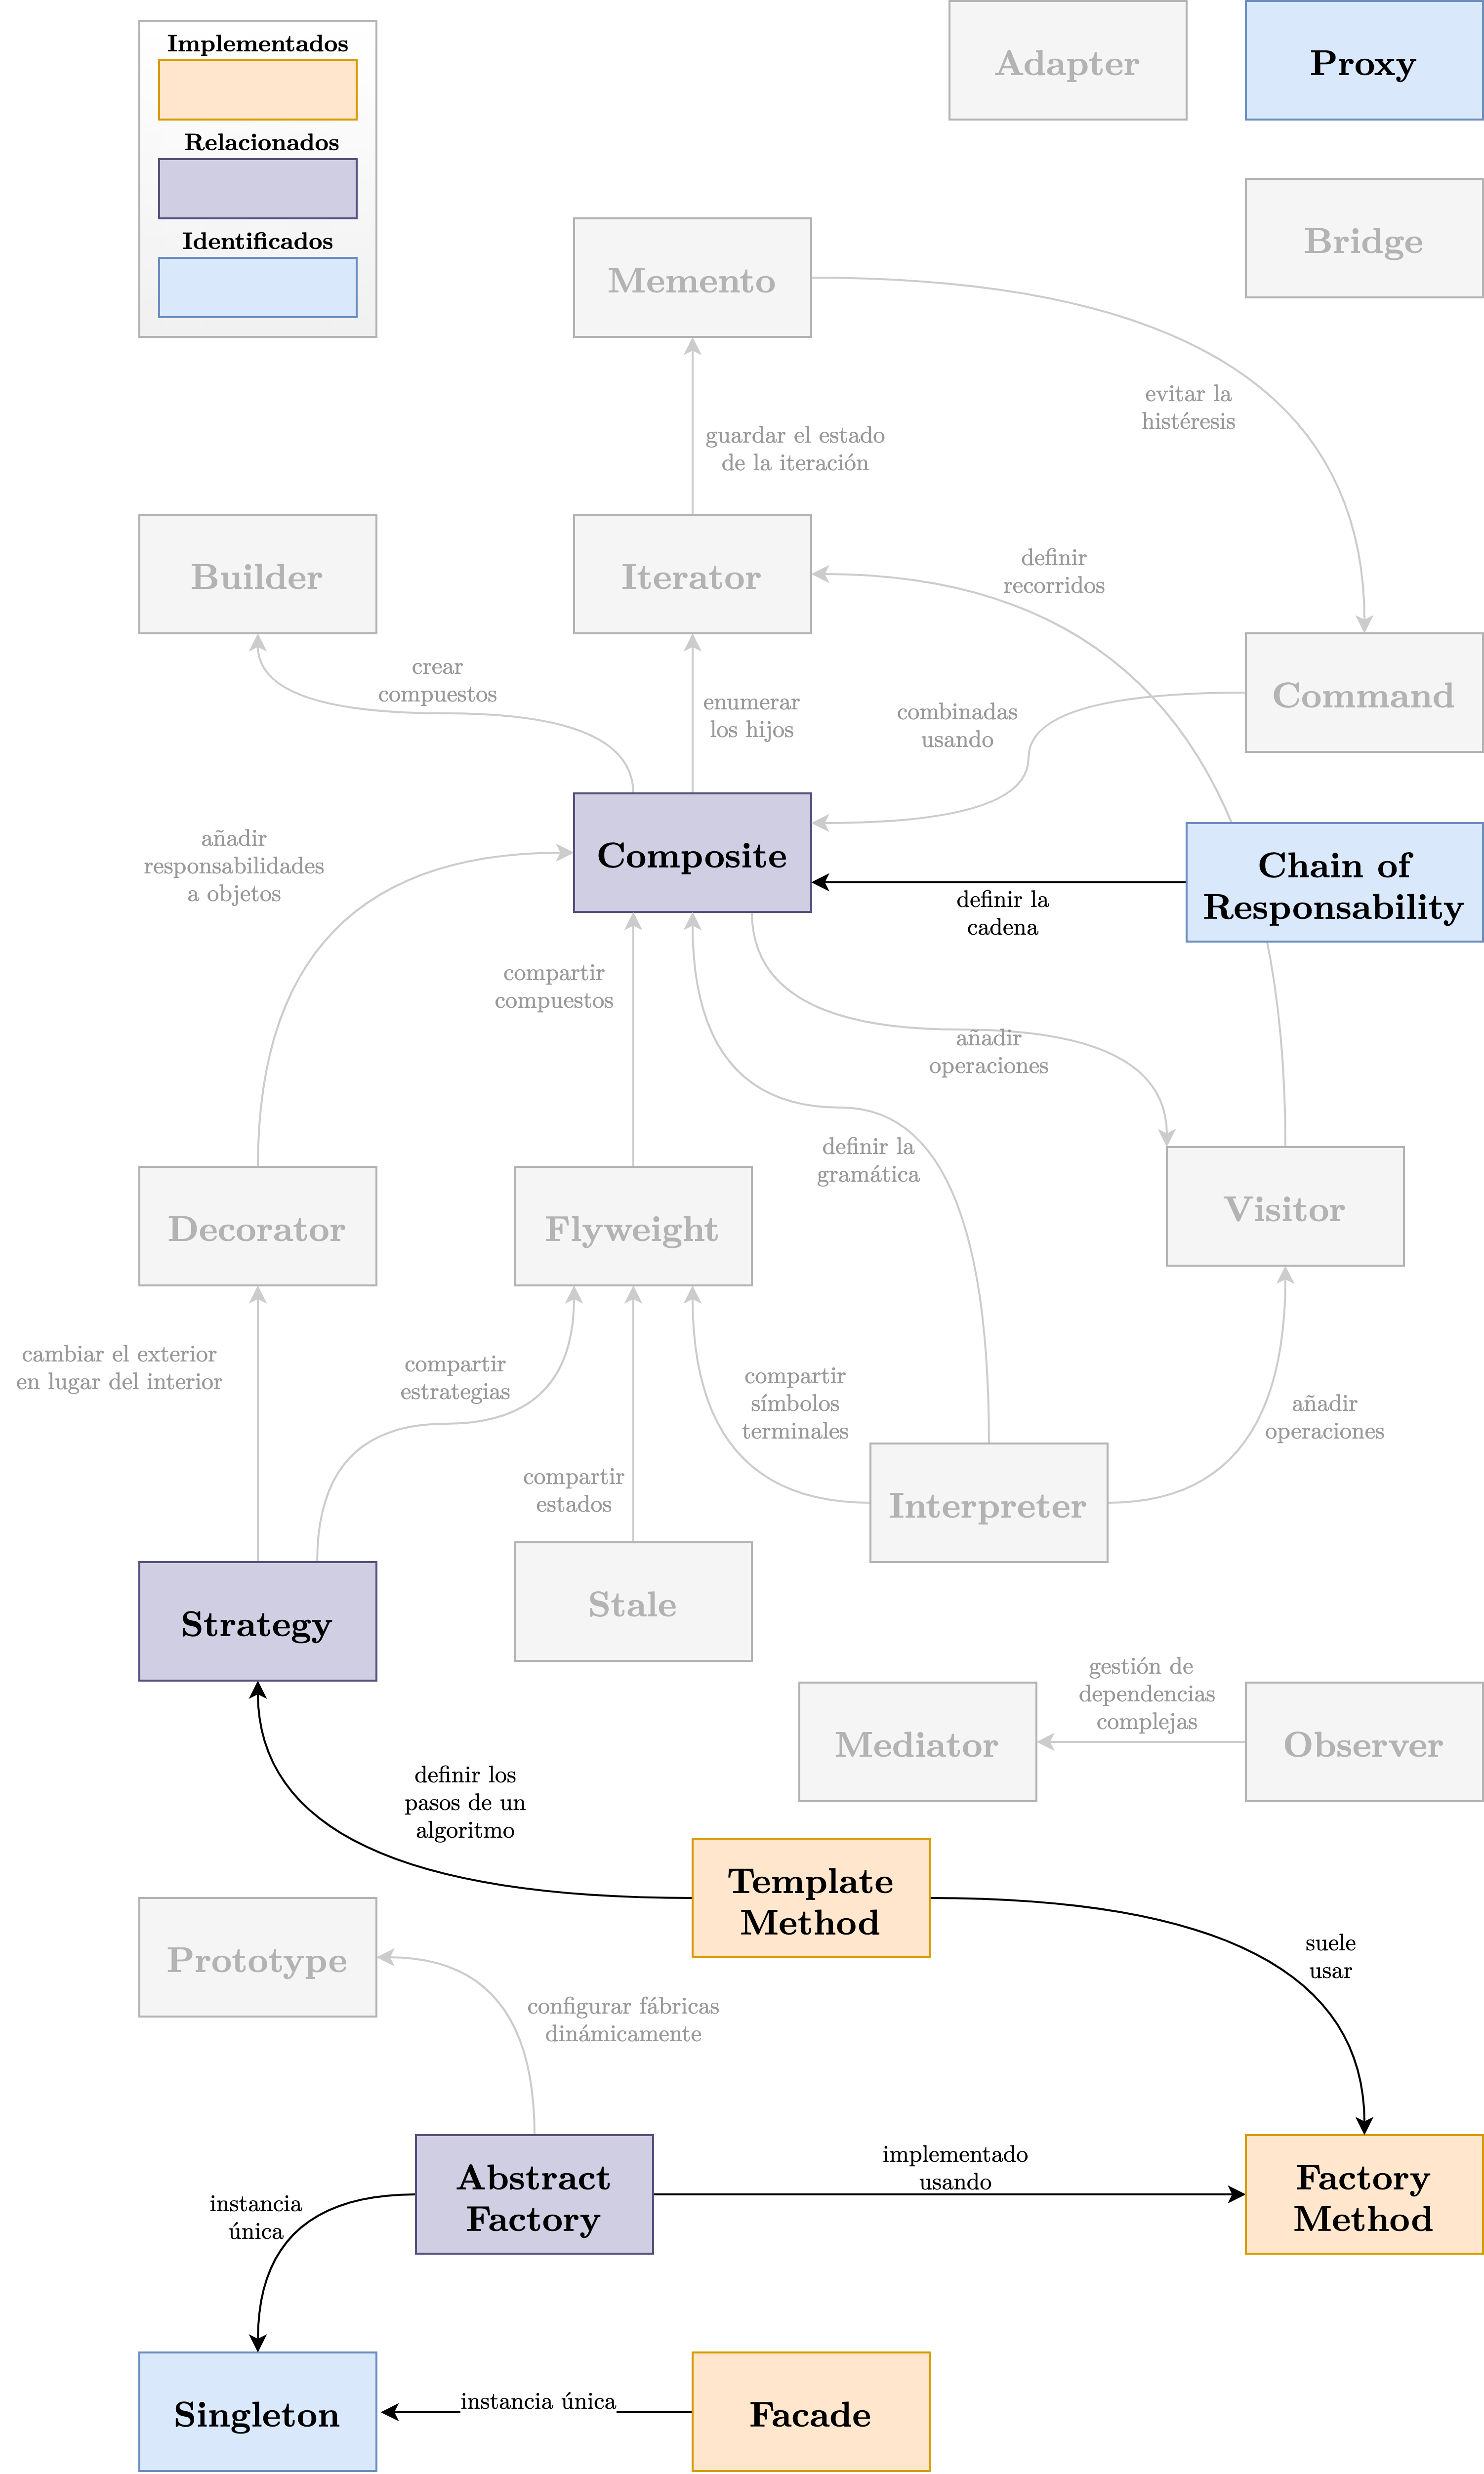
\includegraphics[scale=0.125]{images/PatronesUtilizadosEsquema.png}
                    \end{center}
                \end{figure}
            
                    \subsubsection{Patrones identificados}
                        Aquí se recogen los patrones que están ya implementados en parte del software que se ha utilizado para llevar a cabo el proyecto. El uso de los mismos ha servido para simplificar ampliamente el trabajo en este proyecto.
            
                        \paragraph{Patrón Proxy}
                        El uso de este patrón estructural nos ha resultado útil para optimizar el rendimiento y elasticidad de nuestro servicios ante peticiones repetidas.\\
            
                        Utilizamos este patrón en todos las clases que utilizan la base \texttt{BaseApi} para realizar peticiones a \textit{APIs REST}. La clase en sí actúa como un \textit{proxy} remoto, dando acceso a la \texttt{API} como una clase normal. El método \texttt{getData} actúa como un \textit{proxy} virtual mediante el uso de la anotación \texttt{JCABI Cacheable}. Esta, durante el momento de la compilación, genera un \textit{proxy} del método aplicando técnicas de memoización, llamando al método real sólo cuando es estrictamente necesario.\\
                        
                        Una posible mejora para estos  tipos de servicios, que aplicaría de nuevo este patrón, sería aplicar también el patrón de \textit{proxy} de protección. Por ejemplo, limitando las peticiones por segundo, asegurarnos así que el servicio no se quede sin cuota para otros de usuarios que quieran utilizarlo.
            
            
                        \paragraph{Patrón Dependency Inversion}
                        El patrón \textit{dependency inversion} nos ha resultado útil para desacoplar los componentes de alto y bajo nivel, dado lugar a una implementación más flexible y configurable.\\
            
                        Utilizamos este patrón en las clases que se encargan de gestionar grupos de clases, por ejemplo el \texttt{ServiceManager}. Mediante la inyección de dependencias que proporciona el framework de \texttt{Spring}, el gestor nunca define explícitamente las clases que gestiona, simplemente se le inyectan todas las clases que comparten una interfaz común. Así uno solo se tiene que preocuparse de crear servicios y no de gestionar los, ya que estos se añaden automáticamente al gestor sin ninguna modificación a ninguna de las partes involucradas.
            
                        \paragraph{Patrón Singleton}
                        El patrón \textit{singleton} nos ha resultado útil para centralizar, y por tanto optimizar nuestros servicios, al limitar la manera de acceder a ellos.
            
                        Utilizamos este patrón en todas las clases que vienen anotadas con la anotación \texttt{Spring Service}. Por ejemplo, al aplicarlo a todos los servicios que abstraen \texttt{APIs} nos aseguramos que cada \texttt{API} tiene una, y solo una, representación interna única. Esto nos permite aplicar el patrón \textit{proxy}, mencionado antes, globalmente. Sin ello aplicar las optimizaciones del \textit{proxy} teniendo cuando uno tiene múltiples instancias de la misma API pierde toda su efectividad.
            
                    \subsubsection{Patrones implementados}
                    Los siguientes patrones son aquellos que, hemos implementado de cero, y hemos utilizado ampliamente para simplificar nuestro proyecto.
            
                        \paragraph{Template Method}
                        El patrón de \textit{template method} nos ha resultado útil para abstraer los pasos comunes que tiene que realizar uno para acceder a una \textit{API REST}, sobre todo al tratarse de un proyecto que tiene que integrar multitud de ellas.\\
            
                        Utilizamos este patrón en la clase \texttt{BaseApi}, está implementa parcialmente el algoritmo básico; construir la petición, realizar la petición, validar la respuesta y filtrar los datos. Después, esta se especializa en las clases \texttt{BaseService} y \texttt{BaseQuery}, añadiendo un tipado concreto y algunos atributos. Finalmente siendo implementando en \texttt{NameQuery}, \texttt{CoordsQuery}, \texttt{WeatherService}, \texttt{EventsService}, ...\\
            
                        La única diferencia respecto a la implementación referencia es que el método plantilla getData no es final, esto se debe a una decisión de flexibilidad y optimización. Esto permite a las clases finales anotar el método con anotación \texttt{JCABI Cacheable}, definiendo así las características de memoización que cada una prefiera para su \textit{API} concreta.\\
            
                        Si se quisiera, se podría modificar la implementación para seguir el patrón de manera más estricta, sin embargo esto entraría en conflicto con nuestro objetivo de arquitectura simple.
            
                        \begin{figure}[H]
                            \begin{center}
                            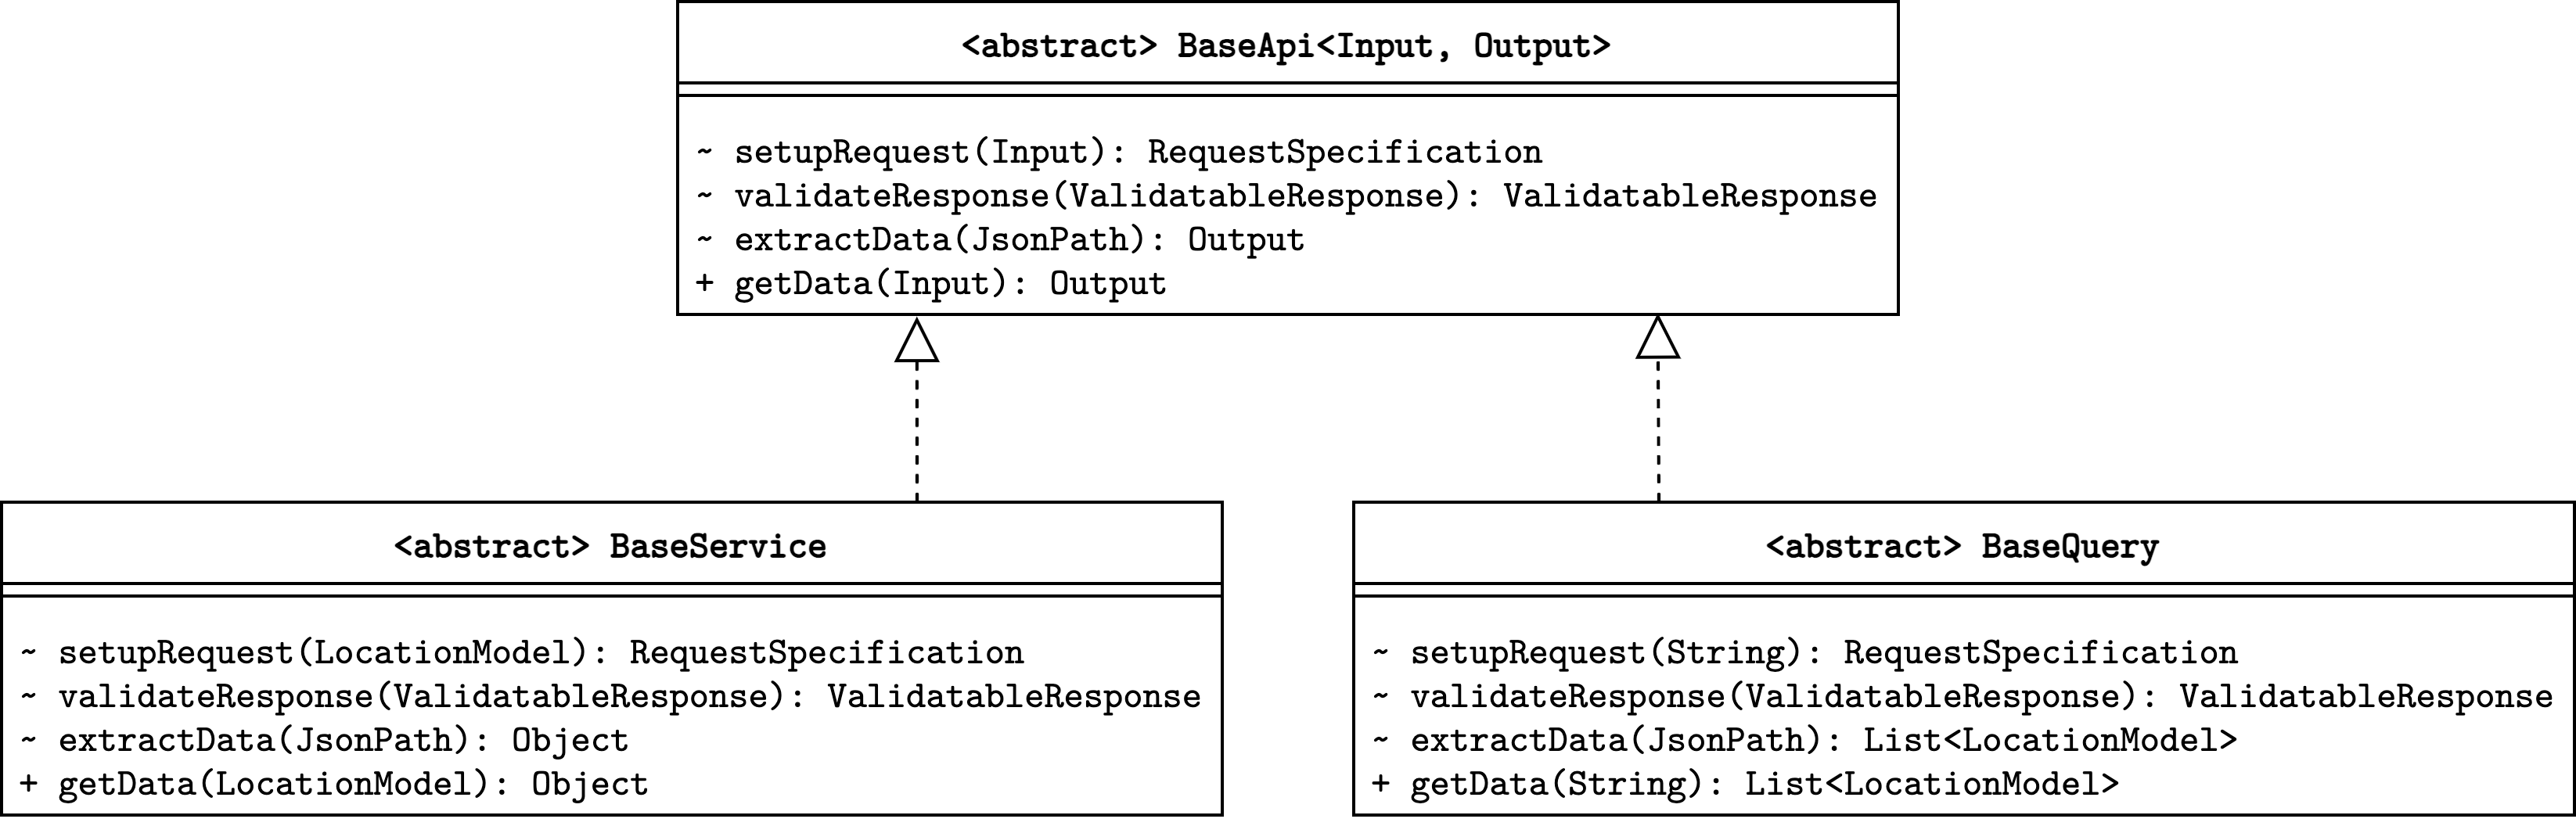
\includegraphics[scale=0.135]{images/TemplateMethod.png}
                            \end{center}
                            \caption{Esquema de \texttt{Template Method}}
                        \end{figure}
            
                        \newpage
                        \textbf{Implementación de \texttt{Template Method}}:
                        \lstinputlisting[language=java, linerange=84-89, firstnumber=84, caption={\texttt{BaseApi.java}}]{code/patterns/BaseApi.java}
            
            
            
                        \paragraph{Factory Method}
                        El patrón \textit{factory method} nos ha resultado útil para desacoplar la creación de instancias del uso de las mismas en multitud de lugares.\\
            
                        Utilizamos este patrón en las clases de \texttt{AccountManager} y \texttt{BaseQuery}, entre otras. Moviendo la responsabilidad de la creación de las clases que implementan la lógica de negocio a las que luego las gestionan.\\
            
                        Por ejemplo, en vez se crea la instancia de \texttt{AccountModel} en la clase que recibe la petición de dar de alta un usuario; lel gestor de cuentas, que es el encargado encargada de gestionar su almacenamiento, es la encargada de crearla también. Así la acción de crear se gestiona de la misma manera que se gestionan el resto de acciones relacionadas.
            
                        \begin{figure}[H]
                            \begin{center}
                                \hspace*{-4mm}
                            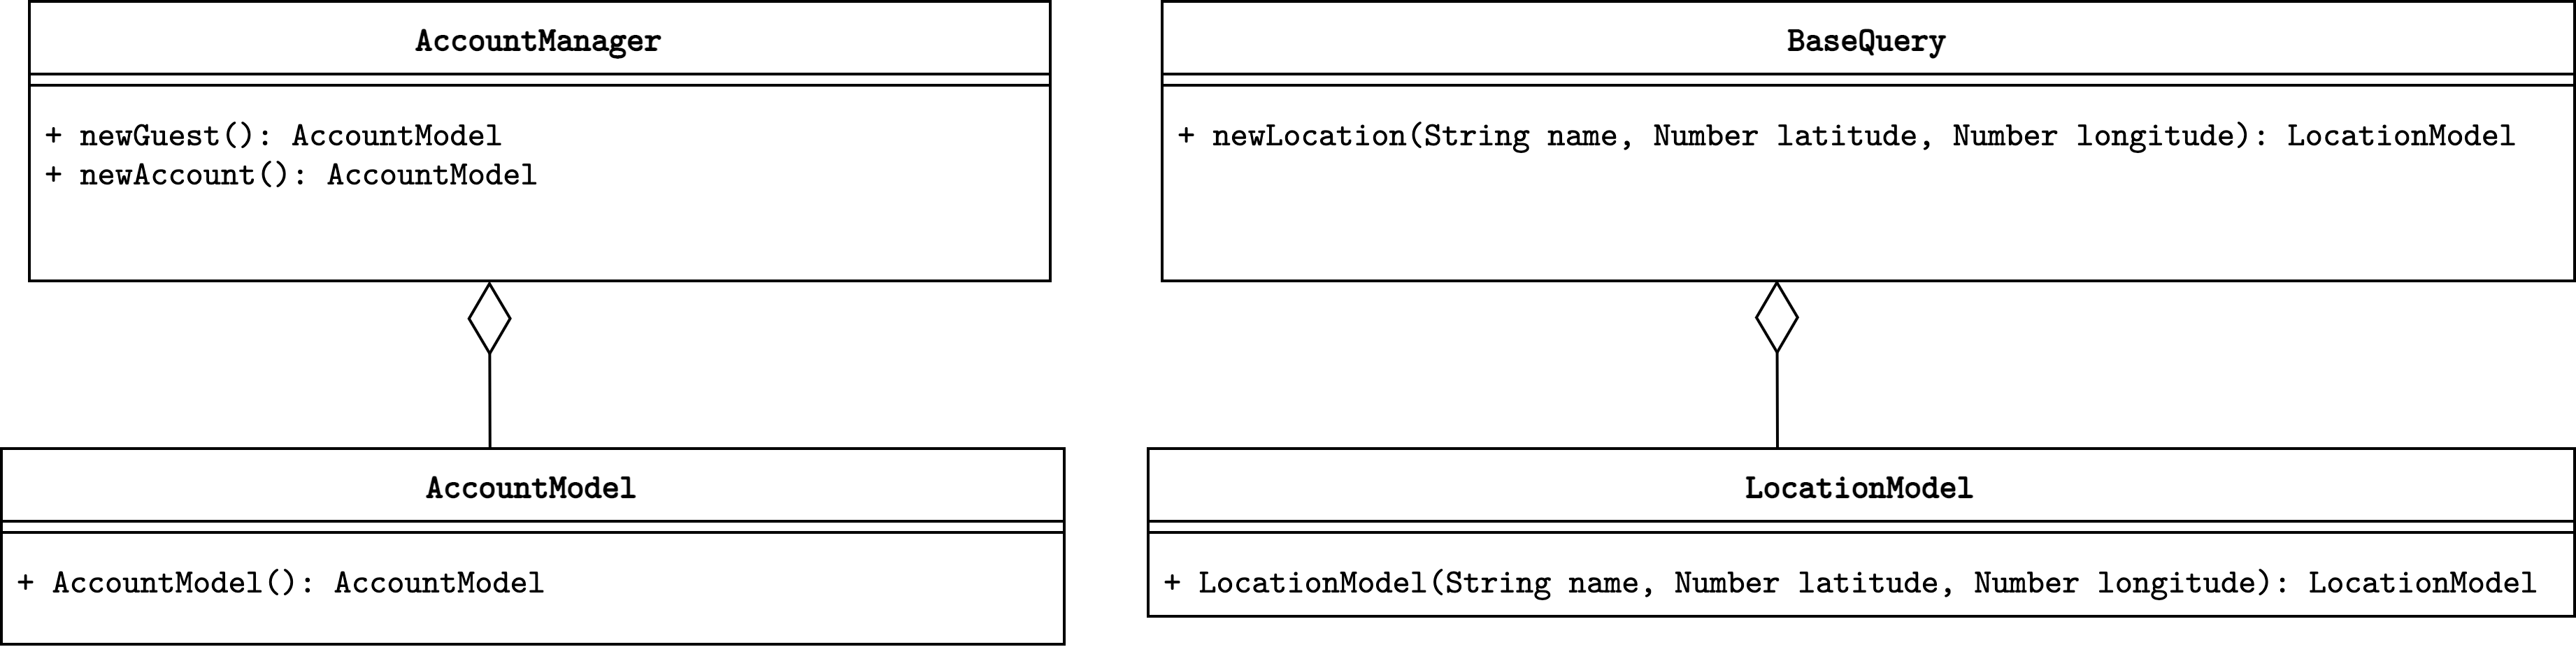
\includegraphics[scale=0.125]{images/FactoryMethod.png}
                            \end{center}
                            \caption{Esquema de \texttt{Factory Method}}
                        \end{figure}
            
                        \textbf{Implementación de \texttt{Factory Method}}:
                        \lstinputlisting[language=java, linerange=18-26, firstnumber=18, caption={\texttt{AccountManager.java}}]{code/patterns/AccountManager.java}
            
                        \lstinputlisting[language=java, linerange=9-11, firstnumber=9, caption={\texttt{BaseQuery.java}}]{code/patterns/BaseQuery.java}
            
            
            
                        \paragraph{Facade Method}
                        El patrón \textit{facade} nos ha resultado útil para simplificar el acceso simultáneo a grupos de varias clases para lograr un objetivo concreto. Necesitando implementar varios servicios por multitud de motivos este problema ha surgido rápidamente.\\
            
                        Utilizamos este patrón en la mayoría de clases de gestión, sin embargo el mejor ejemplo de este es la clase \texttt{QueryManager}. Esta proporciona un método que traduce cualquier tipo de entrada (coordenadas, topónimos, ...) en uno o varios objetos \texttt{LocationModel}. Eliminado así la necesidad de saber el tipo concreto de dato introducido y que servicios harían falta para extraer la información necesaria; así, uno se puede centrar en lo que quiere hacer con ella en vez del cómo obtenerla.
            
                        \begin{figure}[H]
                            \begin{center}
                            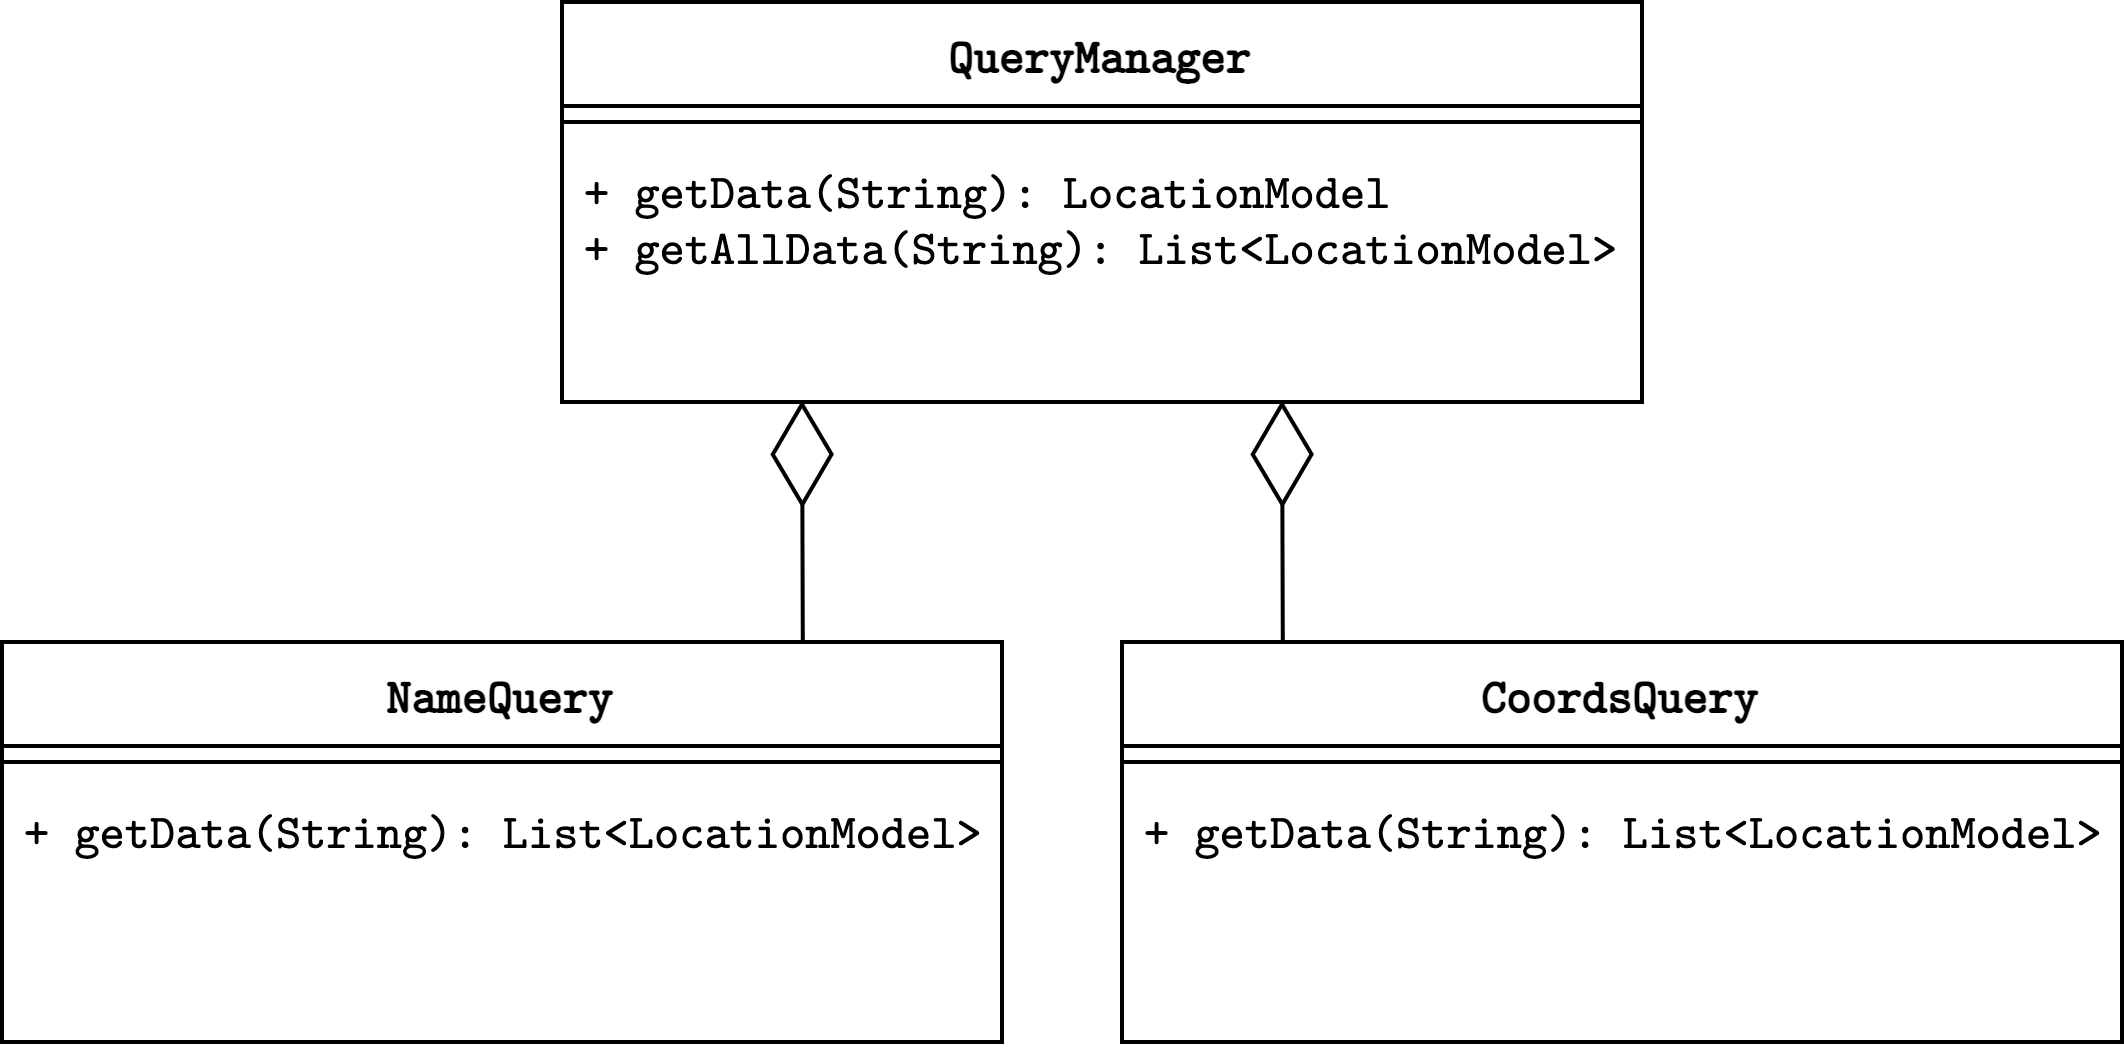
\includegraphics[scale=0.16]{images/FacadeMethod.png}
                            \end{center}
                            \caption{Esquema de \texttt{Facade Method}}
                        \end{figure}
            
            
                        \textbf{Implementación de \texttt{Facade}}:
                        
                        \lstinputlisting[language=java, breaklines=true, linerange=20-26, firstnumber=20, caption={\texttt{QueryManager.java}}]{code/patterns/QueryManager.java}


                        \subsection{Pruebas}

                        Debido a nuestra decisión de integrar todos los componentes posibles en todo momento, excepto la interfaz de usuario, y a las tecnologías que utilizamos hemos tenido que tomar ciertas decisiones de diseño para facilitar su desarrollo.\\
                        
                        Primero, en todos los tests, tanto de aceptación como integración, siempre se espían todos los componentes necesarios para cualquier otra prueba de la batería. Eso se debe a una optimización en la ejecución de las mismas.\\
                        
                        Al integrar el \textit{framework} de \textbf{Spring} y utilizar su inyector de dependencias uno ha de intentar minimizar los cambios en el sistema, refiriéndose con eso a intentar no variar si una misma clase es un \textit{mock} o no dependiendo del test. Esto se debe a que si uno lo cambia, el sistema automáticamente reinicia todo el contexto de la aplicación, algo que toma como mínimo unos 5s. Entonces si uno cambia la definición del sistema por cada test y uno tiene unos 50 tests, eso son unos 4min solo esperando a que empiecen a ejecutarse. Definiendo siempre como espía todo lo que puede hacer falta, solo hay una definición del sistema y por lo tanto solo una pausa de 5s y seguido de ejecuciones continuas.\\
                        
                        También el motivo de utilizar objetos espías en lugar de \textit{mocks} se debe a su alta configurabilidad. Teniendo esa misma definición del sistema, podemos decir si usar el comportamiento real o reemplazarlo dinámicamente durante la ejecución. Esto puede ser bien porque en las pruebas de integración nos interese solo reemplazar cierta parte de un mismo servicio, como las peticiones reales, pero no su nombre o descripción; o en las pruebas de aceptación mantener la misma definición del sistema pero no modificar ningún comportamiento y utilizar todo el sistema real.\\
                        
                        Además de todo eso, siguiendo con nuestra filosofía de integración completa, no creamos ningún \textit{mock} de la base de datos. Sin embargo, gracias a nuestro sistema gestor de bases de datos y a nuestro requisito avanzado de cuentas, aplicamos una solución diferente para separar el sistema real del de pruebas.\\
                        
                        Las pruebas cuando se ejecutan lo hacen dentro de un perfil de pruebas, esto hace que se el gestor genere una nueva base de datos puramente almacenada en la memoria del sistema. Esto no modifica la base de datos de producción pero mantiene toda la lógica que haría habitualmente, como peticiones \texttt{SQL} o comprobaciones de integridad.\\
                        
                        Además, cada test genera su propio usuario único, por lo que los datos de las pruebas están incluso más aislados unos de otros. Empezando siempre con una base en blanco y siendo eliminados al final de cada una de ellas.

                        \subsection{Diseño gráfico}                    
                    
                            \subsubsection{Identidad propia}
                            La identidad propia de una marca es el conjunto de los rasgos que definen los valores y la misión de la empresa o la organización a la que hacen referencia. Engloba por tanto, todos los aspectos que sustentan la marca, tanto en términos visuales como en experiencia y en principios. Algunos de los objetivos de mayor importancia son: crear un factor diferenciador al comparar con la competencia nuestra marca y gracias a ello, posicionarnos en el \textit{imaginarium}\footnote{\textbf{Imaginarium}: Imagen simbólica a partir de la que se desarrolla una representación mental.} de los consumidores.\\
                            
                            El objetivo fundamental es hacer uso de estos elementos visuales y físicos para crear una buena impresión a los clientes o a los usuarios finales a los que va dirigida nuestra aplicación. En conjunto, la identidad de marca engloba los siguientes apartados:
                                \begin{enumerate}
                                    \item Misión, visión y valores.
                                    \item Experiencia del cliente.
                                    \item Logotipo.
                                    \item Selección de color.
                                    \item Tipografía.
                                \end{enumerate}
                            
                            \paragraph{Misión, visión y valores}
                            En el caso de nuestra marca, el \textit{branding} es de vital importancia, puesto que al tratarse de una aplicación (en un \textit{futurible} descargable desde una tienda de aplicaciones), debe lidiar con una gran competitividad por parte de aplicaciones que realizan funciones similares. Es por ello, por lo que antes de empezar con el diseño del logotipo, colores, branding e incluso elementos tipográficos, debemos tener en cuenta cual es la misión, visión y valores de la aplicación que vamos a implementar.
                            
                            \begin{itemize}
                                \item Información
                                \item Previsión
                            \end{itemize}
                            
                            \paragraph{Experiencia del cliente}
                            Esta aplicación aspira a tener una experiencia de navegación minimalista, organizada y límpia, de forma que el usuario final tenga a su disposición toda la información de manera rárpida y sencilla. \\
                    
                            Hoy en día, se puede decir que la habilidad de una marca para entregar una buena experiencia a sus usuarios, constituye una ventaja competitiva. En nuestro caso, gracias a la experiencia de usuario, queremos incentivar el uso de esta aplicación a cualquier persona que precise conocer datos meteorológicos, eventos o noticias de forma rápida y sencilla.
                    
                            \paragraph{Logotipo}
                            Con el fin de elegir una imagen corporativa para nuestro proyecto, se ha hecho un abanico de 12 logotipos a partir de plantillas, y entre los elementos del grupo hemos escogido el que consideramos que será óptimo para constituir nuestra imagen como promotores de esta aplicación. \\
                            
                            Los motivos gráficos que hemos seleccionado son esencialmente esquemas visuales que evoquen a elementos que tienen dependencias de otros, es decir, al tratarse de una aplicación que depende de servicios externos \textit{API}, queremos plasmar en el logotipo esta idea de forma que un conjunto de elementos finito, unidos, constituyan un todo.\\
                    
                            Estos fueron los 12 logotipos de los que partimos para elegir el definitivo:
                    
                            \begin{figure}[H]
                                \begin{center}
                                    \hspace*{-5mm}
                                
\includegraphics[scale=0.16]{images/Logos1.png}
                                \end{center}
                            \end{figure}
                            \vspace*{-10mm}
                            \begin{figure}[H]
                                \begin{center}
                                    \hspace*{-5mm}
                                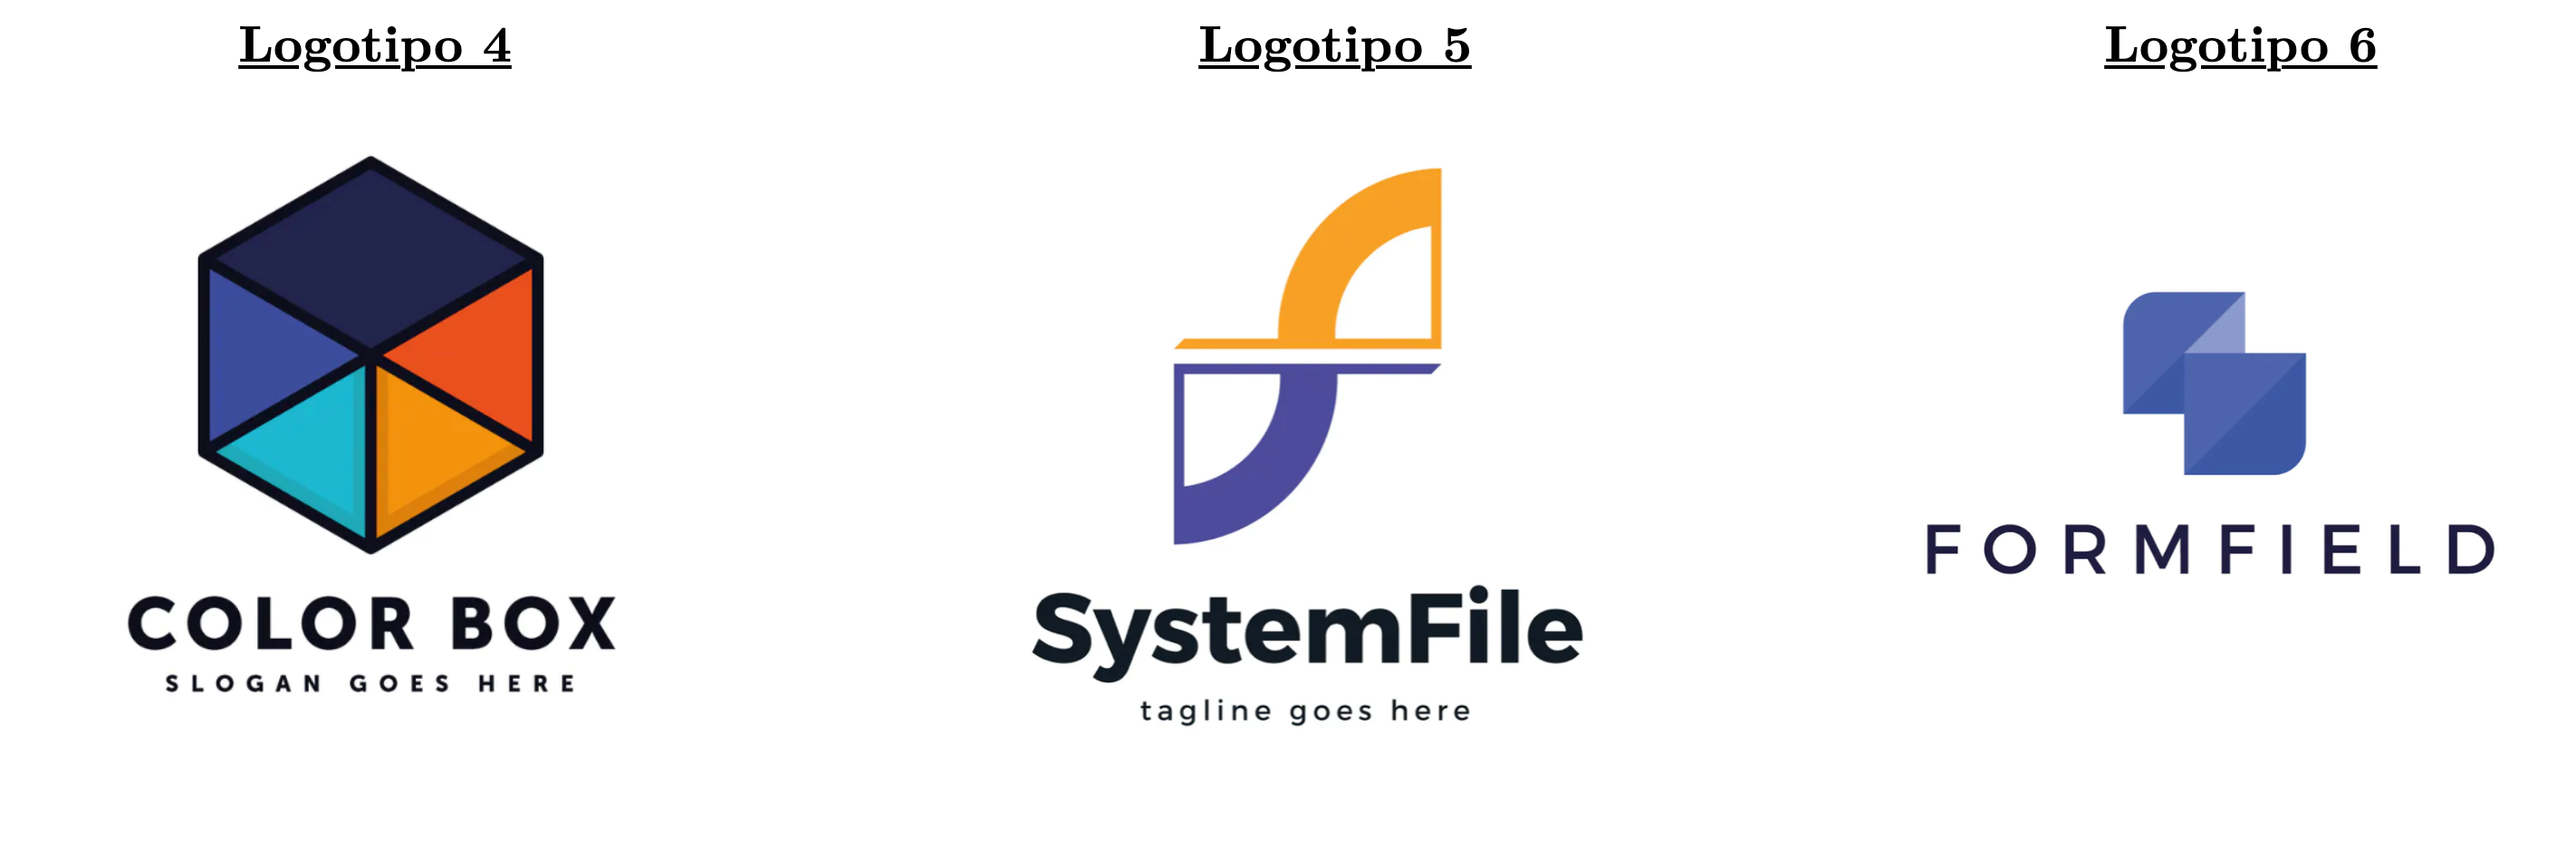
\includegraphics[scale=0.16]{images/Logos2.png}
                                \end{center}
                            \end{figure}
                            \vspace*{-10mm}
                            \begin{figure}[H]
                                \begin{center}
                                    \hspace*{-5mm}
                                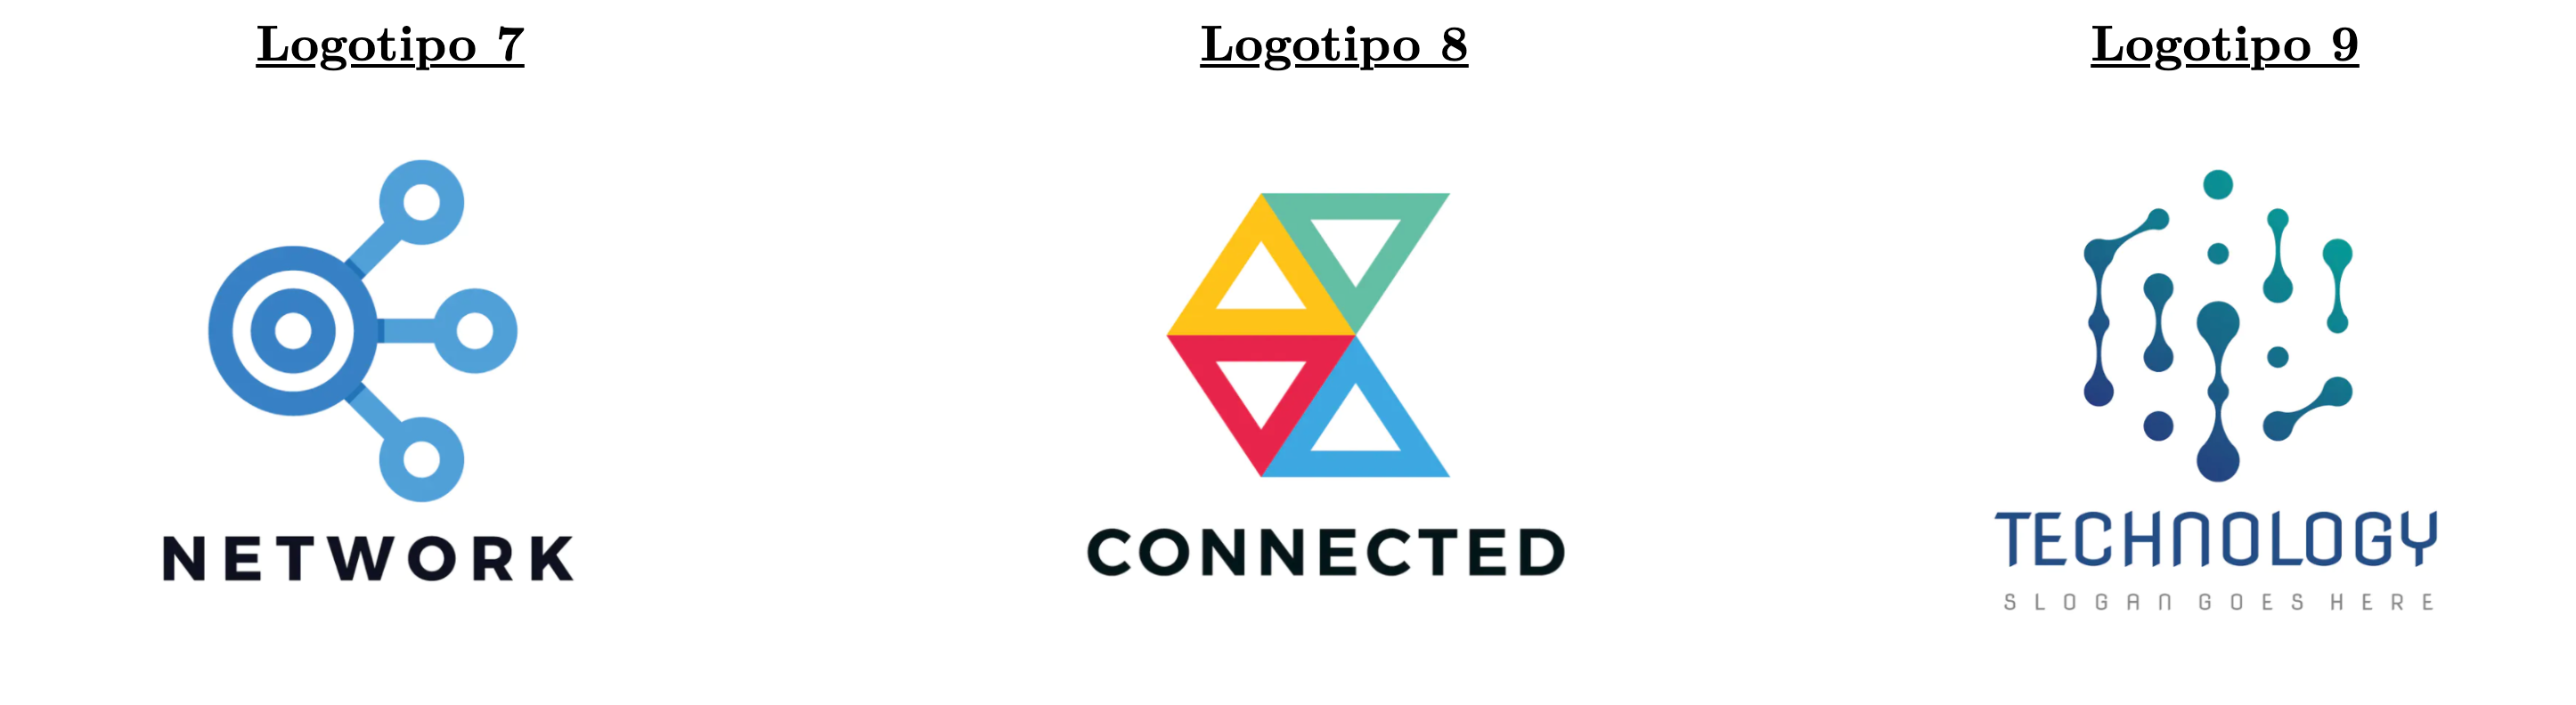
\includegraphics[scale=0.16]{images/Logos3.png}
                                \end{center}
                            \end{figure}
                            \begin{figure}[H]
                                \begin{center}
                                    \hspace*{-5mm}
                                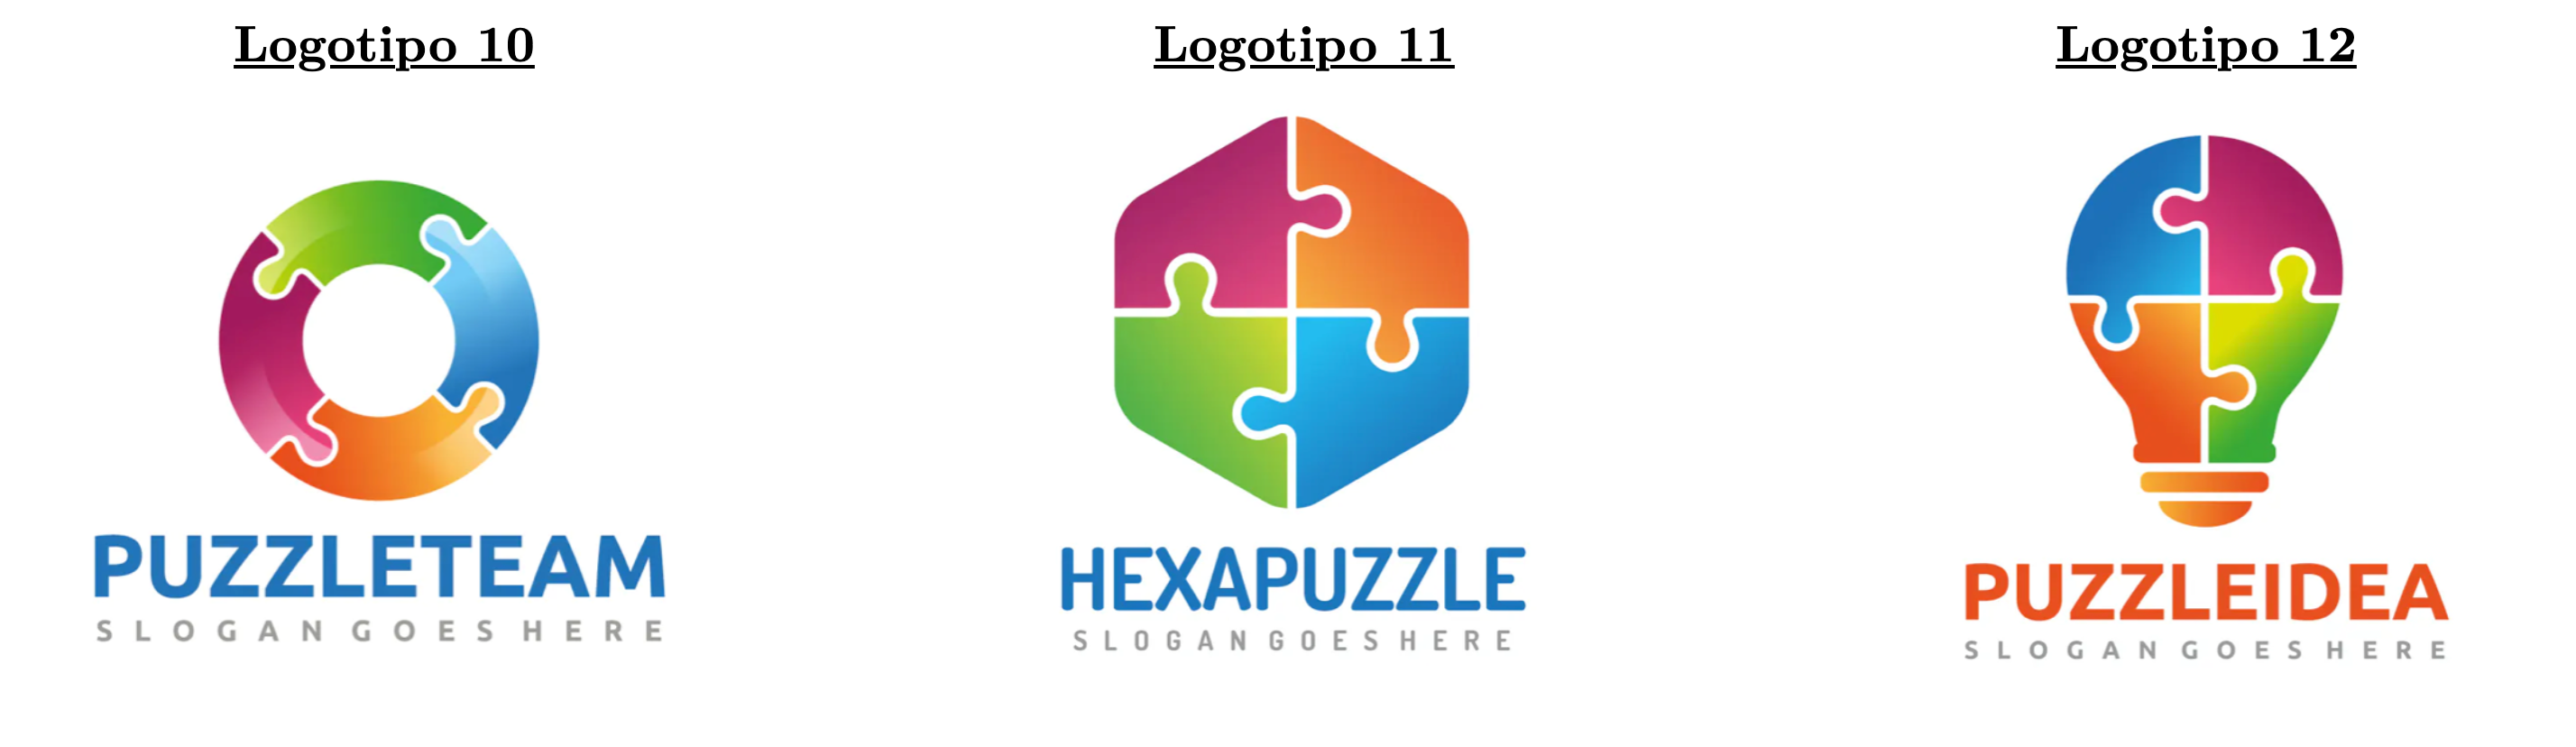
\includegraphics[scale=0.16]{images/Logos4.png}
                                \end{center}
                            \end{figure}
                    
                            Los logotipos con mayor valoración por parte de los elementos del equipo, fueron los logotipos 2, 7 y 11. Internamente hicimos una segunda valoración teniendo en cuenta los objetivos de la aplicación que estamos desarrollando y también las diferentes opciones de reedición que nos permite hacer el logotipo (isotipos, banners, etc), por lo que finalmente como equipo nos decidimos por el uso del logotipo 7.\\
                    
                            El logotipo 7 consta de 4 circunferencias, una de mayor tamaño y otras tres de tamaño más pequeño unidas a la de tamaño grande. Predomina el color azul en el esquema exterior a la figura central y degragado de azul a azul-negro en las subregiones internas no consecutivas de mayor tamaño.\\
                            
                            Este logotipo, por tanto, representa de forma esquemática en esencia el como va a ser nuesta aplicación de forma interna. Tenemos un panel central donde poder elegir una ubicación e internamente van a ser las diferentes API las que obtengan la información necesaria, por lo que el esquema de 3 brazos fue valorado positivamente por el equipo. El texto elegido para este logotipo es \textbf{NEW}: \textbf{N}ews, \textbf{E}vents \& \textbf{W}eather, claramente representado por cada una de las circunferencias exteriores.\\
                    
                            Con este diseño podemos componer 1 isotipo\footnote{\textbf{Isotipo}: Identificador gráfico que por si mismo no requiere ningún texto adicional para definir a la empresa u organización.} (cuando sea necesario el uso del mismo como grafismo en tamaño pequeño: app, icono de app, etc), y 2 versiones completas, que serán de gran utilidad para la representación de este grafismo tanto en la página de inicio de este documento como en secciones de mayor tamaño.\\

                            \newpage
                    
                            A modo de resumen, las características que posee el logotipo que hemos diseñado para este proyecto son:
                                \begin{itemize}
                                    \item \textbf{Colores}: Elevada predominancia del azúl como color vehicular, con degradados a tonos más oscuros en la parte central de la figura. Estos degradados son radiales, por lo que el color de relleno de los puntos exteriores de la misma son claramente más ténues que el de los puntos más lejanos. Se ha optado por el uso de degradado de color para dotar a la figura de mayor volumen.
                                        \begin{itemize}
                                            \item Azul claro (\texttt{HEX}): \texttt{99CCFF} es el que se usa en la mayor parte de la figura, tanto en las circunferencias externas como en los nodos de conexión con la zona central.
                                            \item Azul medio (\texttt{HEX}): \texttt{8AB8E6} es el que se usa en el degradado inicial de la figura central (la parte más externa).
                                            \item Azul oscuro (\texttt{HEX}): \texttt{000099} es el que se usa en el degradado final de la figura central (la parte más interna).
                                        \end{itemize}
                                    \item \textbf{Formato}: El formato de los logotipos es vectorial y en fichero \texttt{.svg} con el fon de poder ampliar y reescalar el logotipo tanto como se requiera sin que pierda calidad. Esta edición y composición se han realizado con Adobe Illustrator 2021.
                                \end{itemize}
                            
                                Las medidas que se muestran en los apartados siguientes están expresadas mediante puntos\footnote{\textbf{Punto (pt)}: es una medida utilizada en tipografía y diseño. Cada punto equivale a $\approx$ \texttt{0,0138} pulgadas.}.
                    
                                \newpage
                            
                            \paragraph*{Isotipo}
                            Este es el isotipo tanto de la apliación como del icono web. Se trata de una versión del logotipo, pero sin texto y se utilizará para encabezamientos breves, como \textit{label} y \textit{shortcut}.\\
                    
                            Nótese que las proporciones de ancho y alto de la figura siguiente son a razón de 9:10 dando en este caso 800 puntos de altura y 720 puntos de ancho. Cada uno de los nodos, están conectados a la circunferencia principal a razón de 45° entre sí. Por lo que los nodos de las secciones A y C tienen un ángulo recto. Se ha acotado únicamente la sección A, puesto que la B y la C són idénticas.\\
                    
                            Por otro lado, y en comparación con el logo inicial, se ha incluido un degradado para dotarde cierto volumen a la figura central. También se han modificado sutilmente el ángulo de unión de los nodos y su longitud.
                    
                            \begin{figure}[H]
                                \begin{center}
                                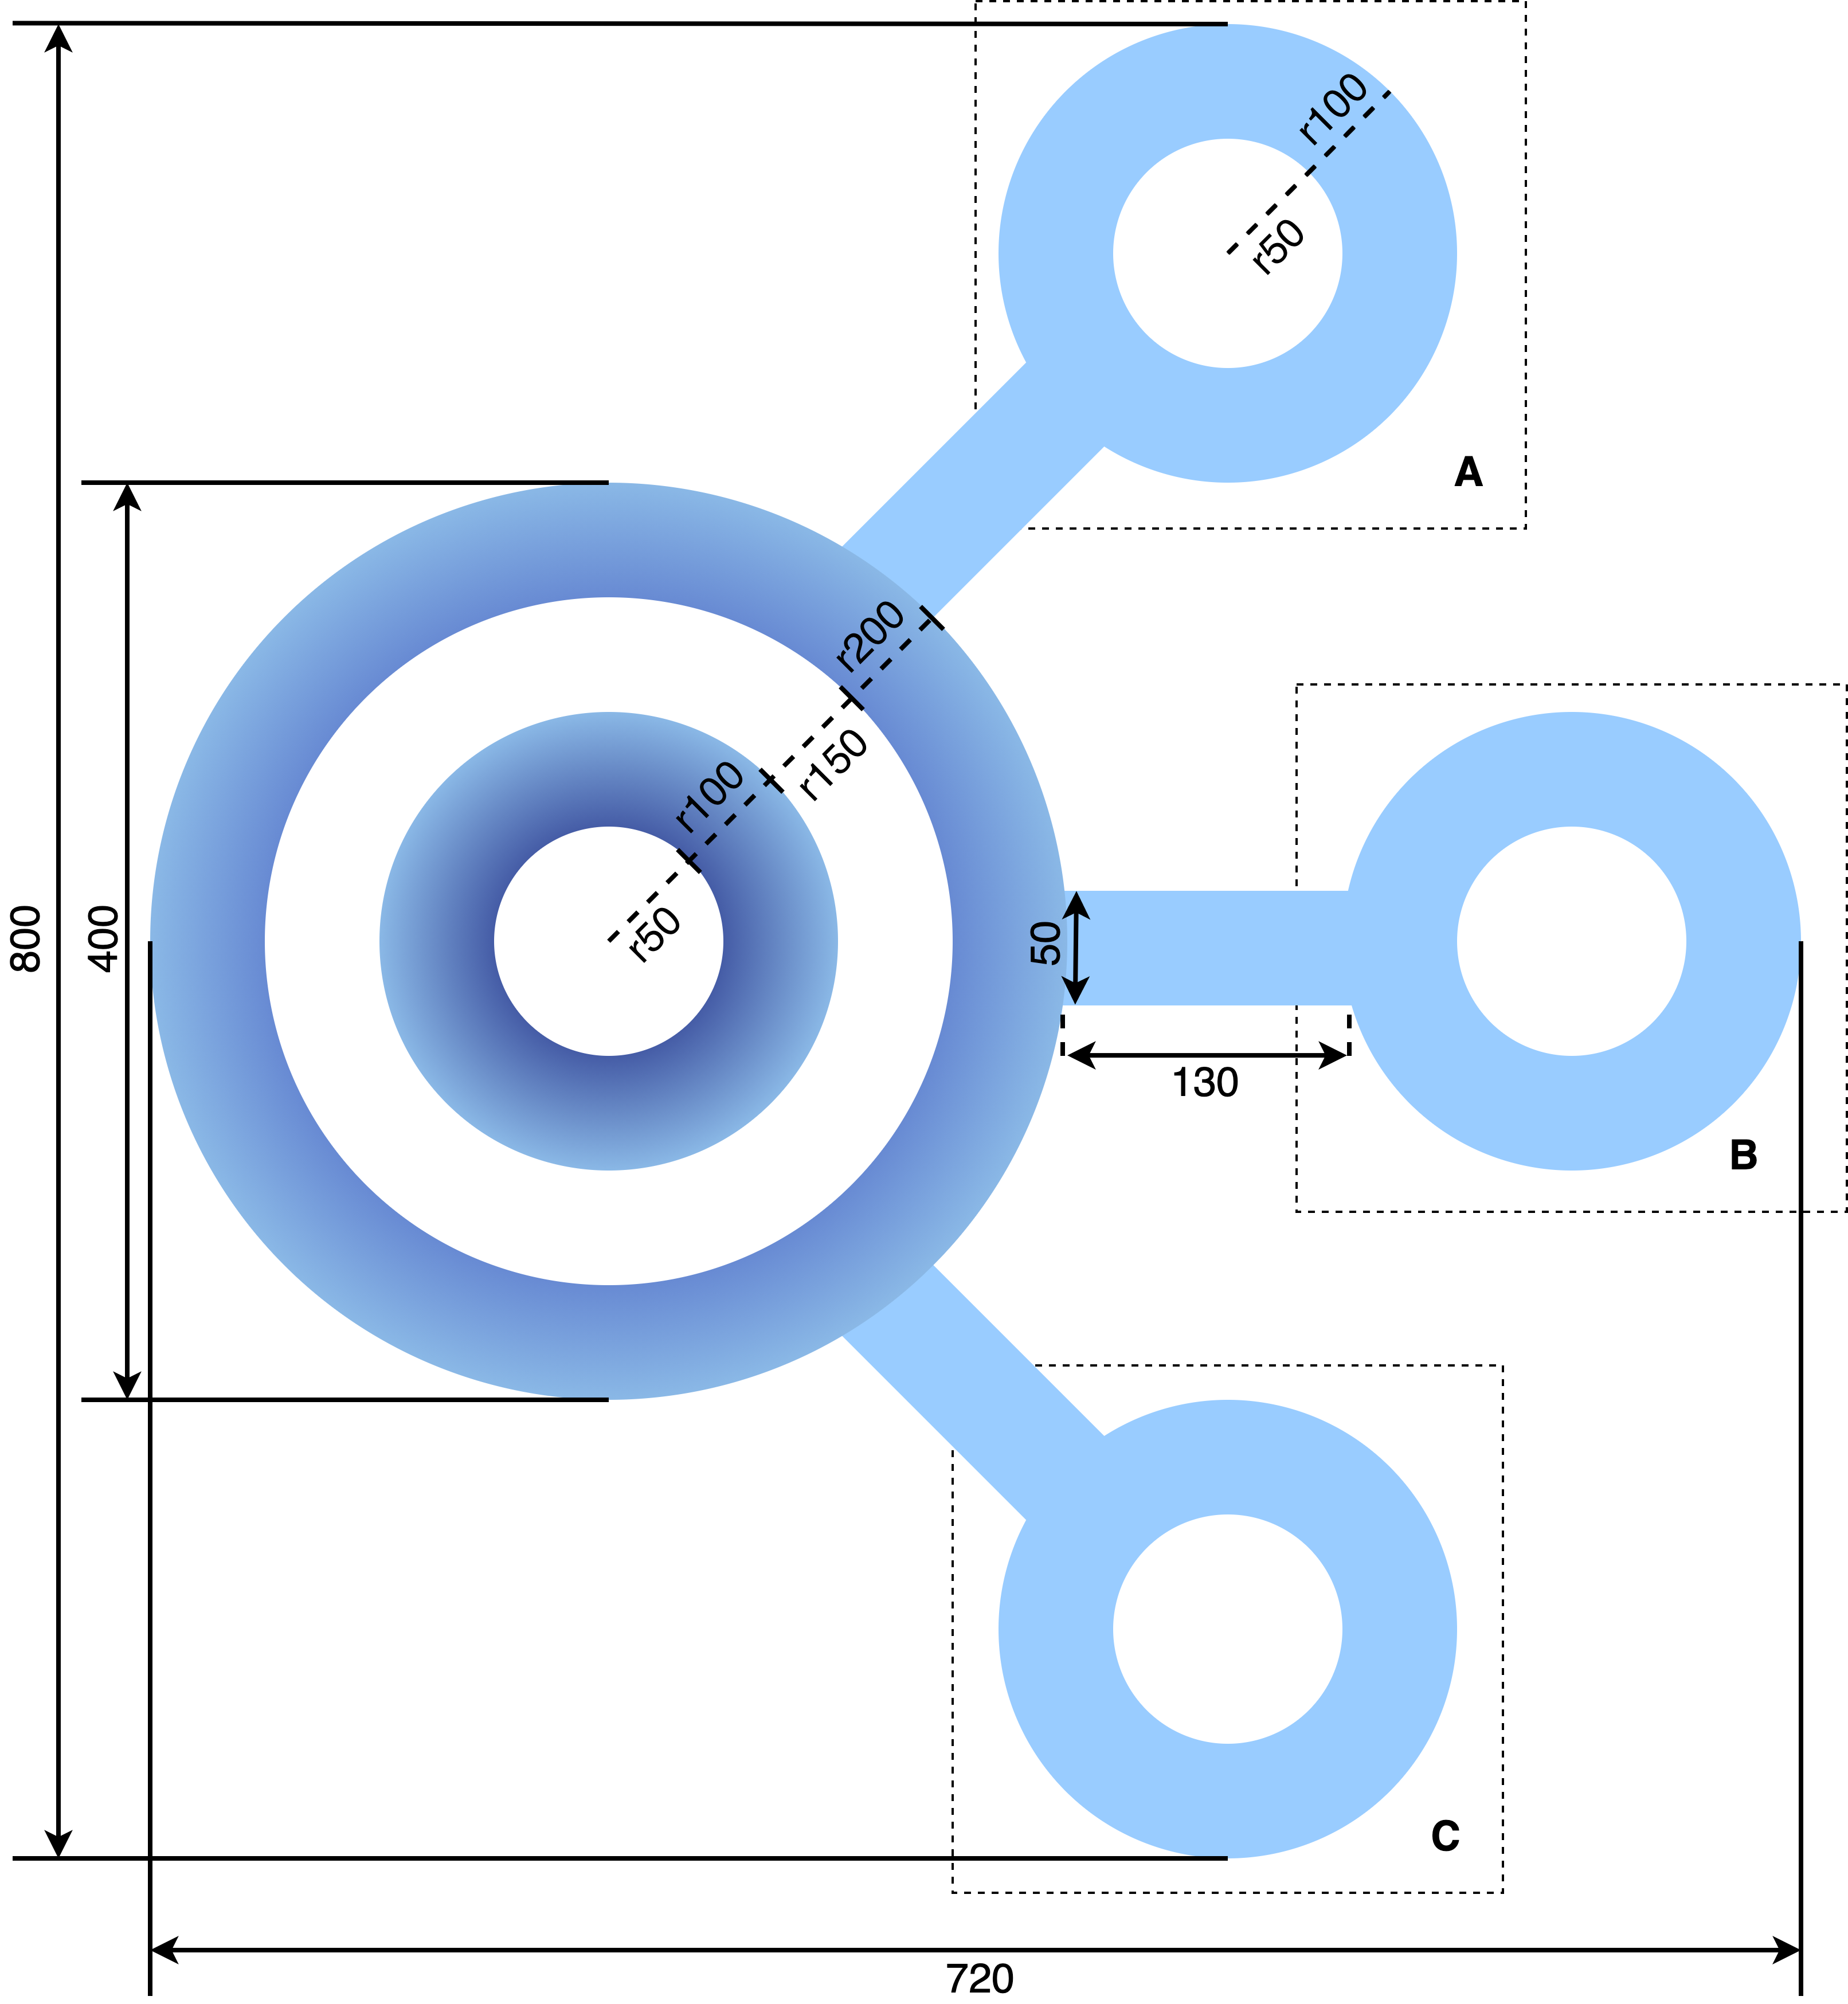
\includegraphics[scale=0.10]{images/LogoIsotipo.png}
                                \end{center}
                                \caption{Isotipo con medidas acotadas (pt.)}
                            \end{figure}


                            \newpage
                    
                    
                            \paragraph*{Imagotipo prinicpal}
                            La siguiente figura hace referencia al imagotipo principal. El cometido de este grafismo es su uso como sello de los documentos de grupo así como el disponer de una versión de mayor tamaño con las siglas de nuestra aplicación.\\
                    
                            En este caso, el imagotipo deriva directamente del isotipo, añadiendo las siglas \textit{NEW} con su descomposición \textit{News}, \textit{Events} y \textit{Weather}, justamente las \textit{API} que utilizamos en el proyecto. Aunque vayamos a comentar la colorimetría en otros puntos, para matener la cohesión del texto con el resto del logotipo, los colores son los mismos que los del degradado de la figura principal.
                    
                    
                            \begin{figure}[H]
                                \begin{center}
                                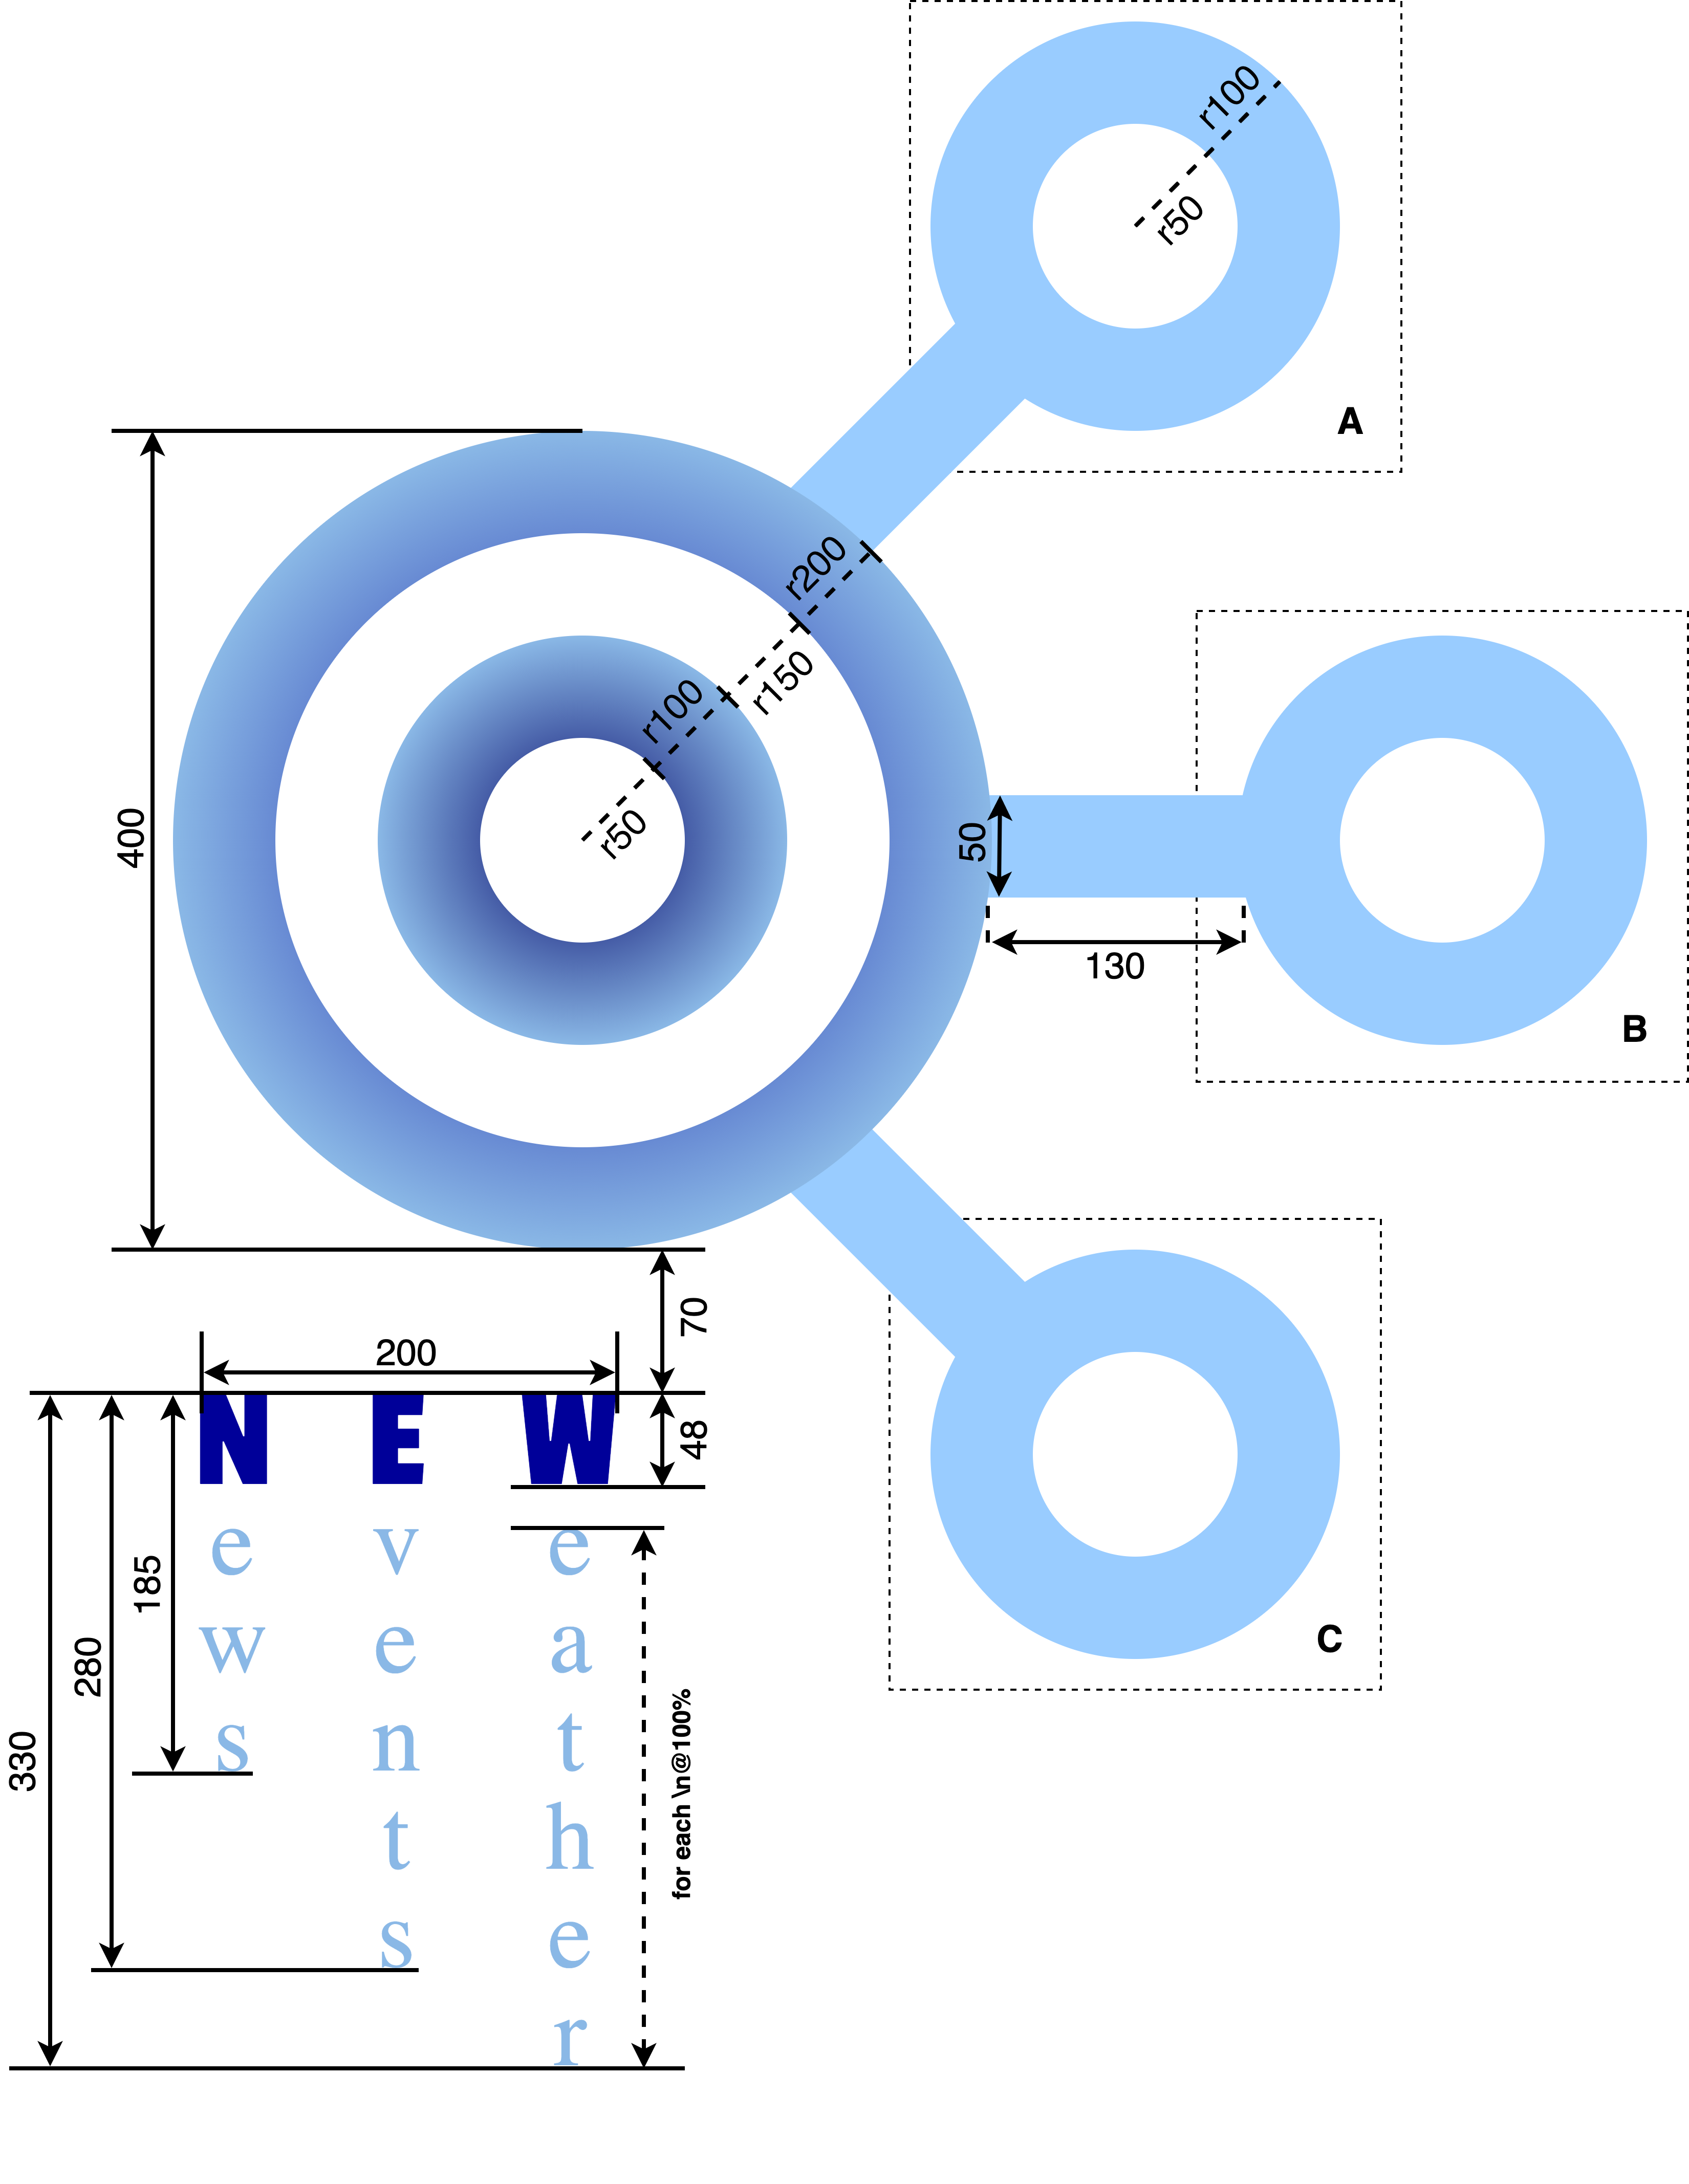
\includegraphics[scale=0.10]{images/LogoAcotadotexto.png}
                                \end{center}
                                \caption{Imagotipo con medidas acotadas (pt.)}
                            \end{figure}
                    
                    
                    
                            \paragraph*{Imagotipo secundario - Banner horizontal}
                            Este es el imagotipo secundario en formato de banner apaisado horizontal. Tal y como se muestra a continuación tiene un fondo degradado naranja-azul, pero este únicamente delimita las fracciones del banner. Este puede ser representado con otro color y delimitación adptandose al \textit{background} en cada ocasión, aunque idelmente debería combinarse con colores complementarios a los 3 tonos de azúl que lo componen.
                    
                    
                    
                            \begin{figure}[H]
                                \begin{center}
                                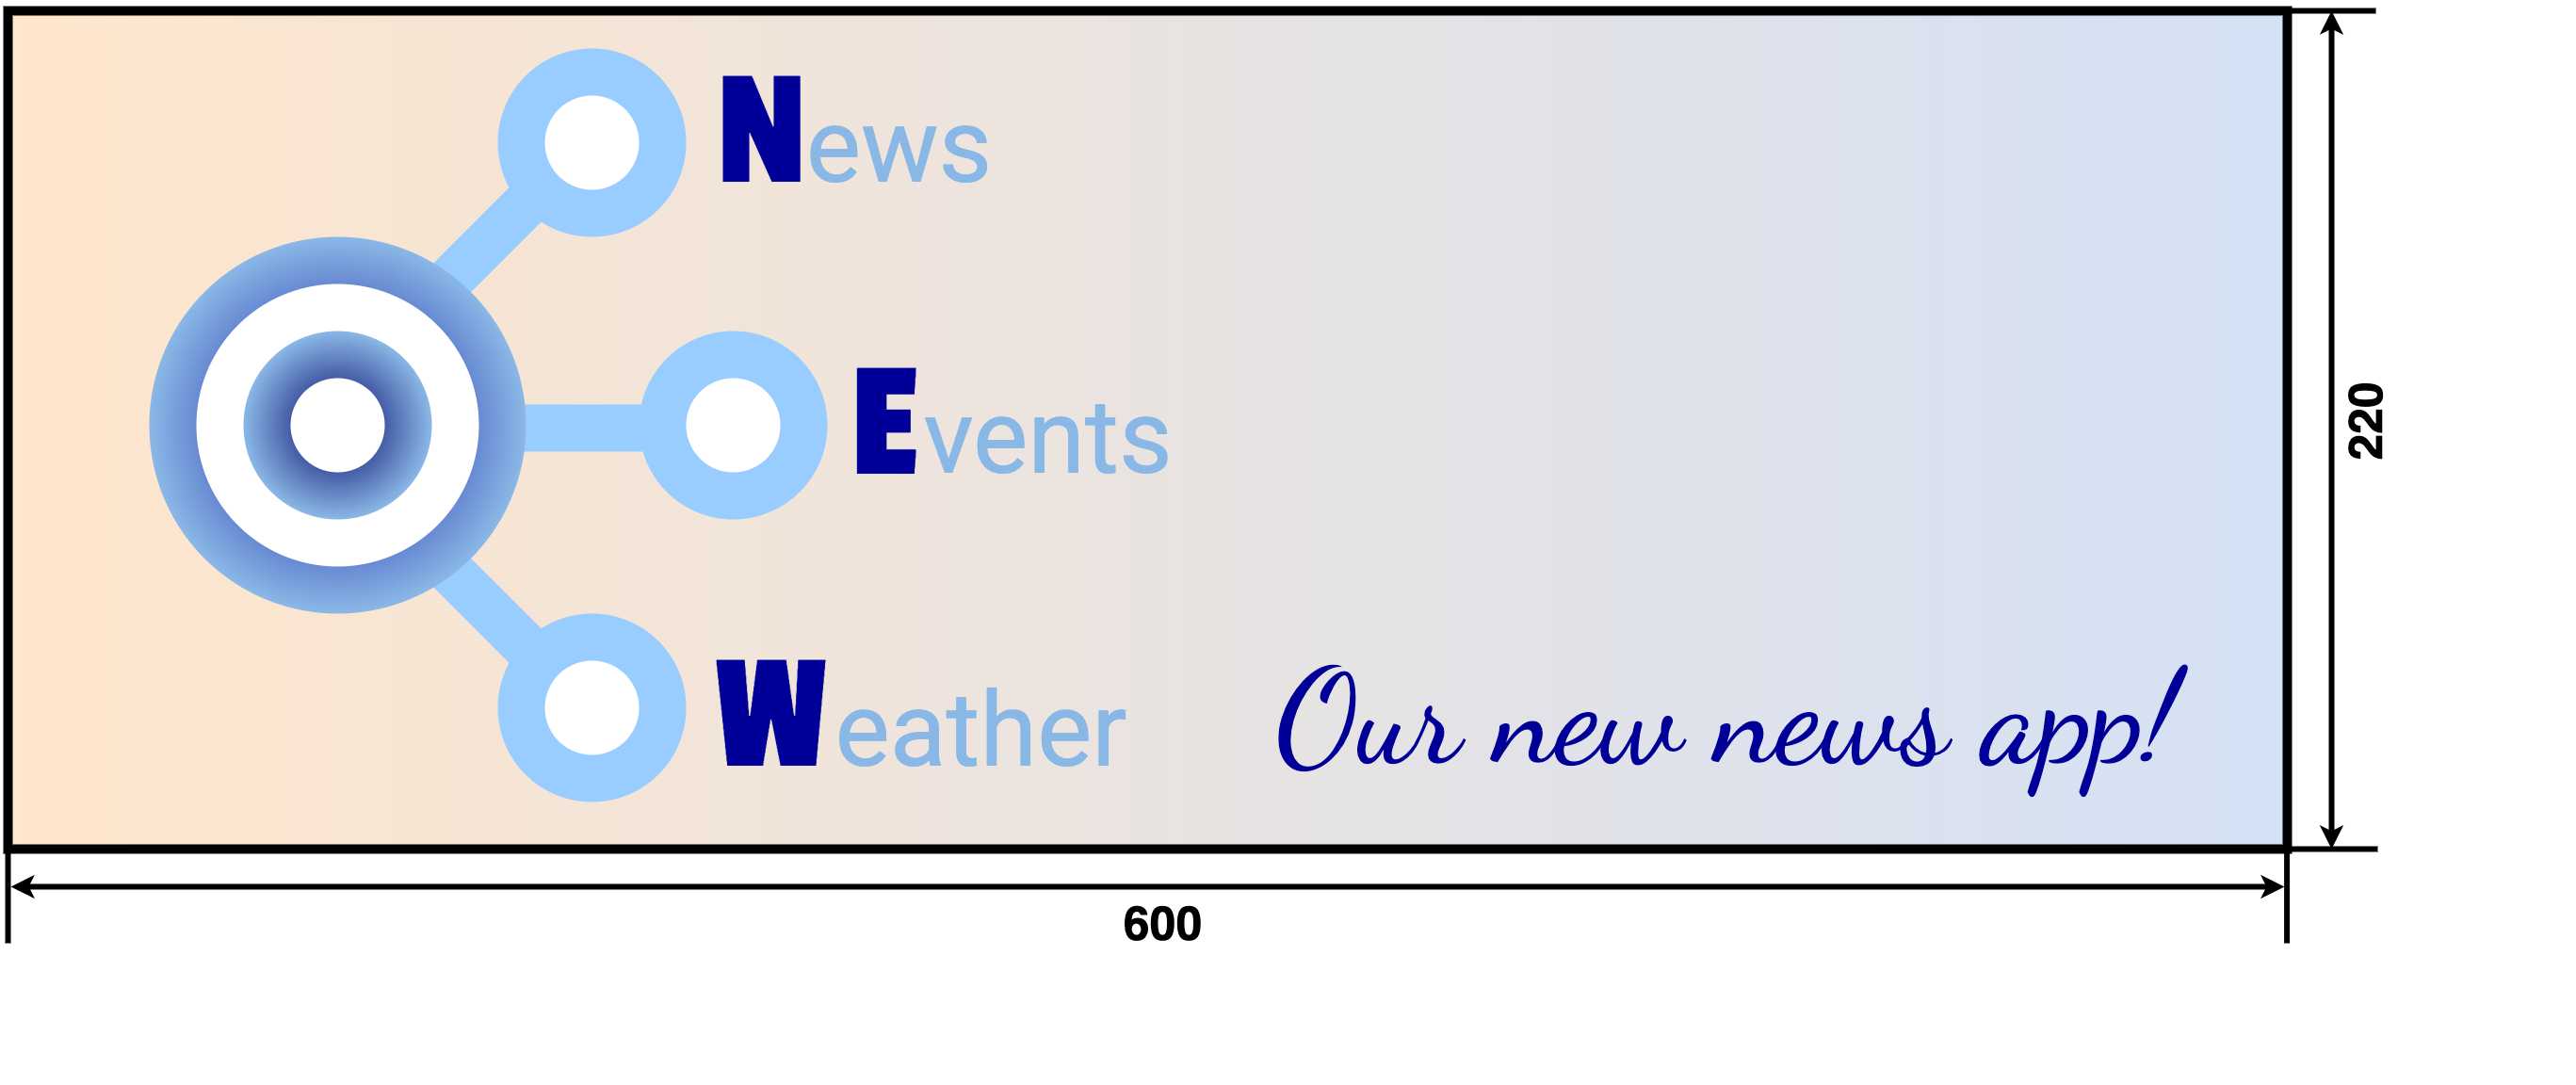
\includegraphics[scale=0.14]{images/LogoBanner.png}
                                \end{center}
                                \caption{Imagotipo Secundario - Banner Horizontal}
                            \end{figure}

                            Finalmente no hemos apostado por el uso de este banner, porque no lo hemos considerado necesario. No obstante, queda en la carpeta de documentos para su uso en un futuro a modo de publicidad o \textit{branding}.
                    
                            \paragraph{Selección de color}
                            Cuando realizamos el diseño de una interfaz visual, escoger una paleta de colores correcta es muy importante, porque esta aporta armonía y complementa la visión de la aplicación (web en este caso).\\
                            
                            Es por eso por lo que a partir del logotipo, y sus motivos principales en este proyecto, hemos finalmente elegido unas tonalidades de azúl (claro, medio y oscuro) para crear contraste y volumen al logotipo a la vez que tratamos que sea lo más minimalista y limpio posible.\\
                            
                            Tal y como se puede apreciar en la figura siguiente, el logotipo tiene únicamente tres tonalidades de azúl. Azúl claro (\texttt{HEX 99CCFF}) para la silueta de los nodos, círculos exteriores y nombres (a excepción de las letras capitales), y un rango de degradado (\texttt{HEX 8AB8E6} $\rightarrow$ \texttt{000099}) para la figura central. El análisis de la composición cromática del logotipo, es:

                            \newpage

                            \begin{center}
                                \underline{\textbf{Paleta de colores: Logotipo}}
                            \end{center}

                            \begin{figure}[H]
                                \begin{center}
                                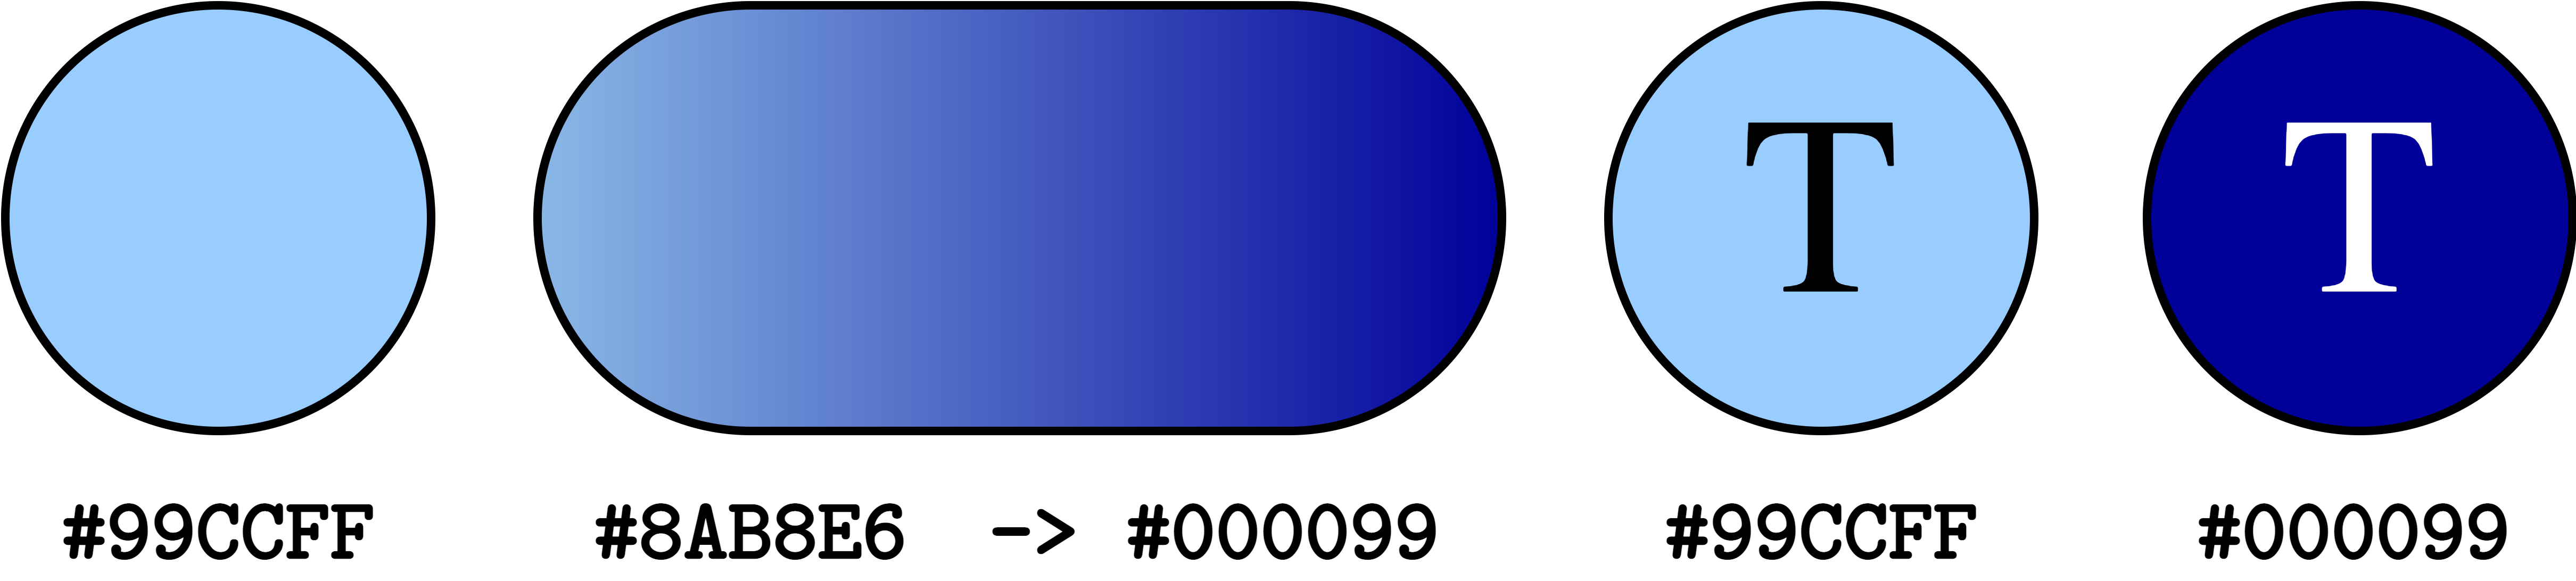
\includegraphics[scale=0.065]{images/ColoresLogoEsquema.png}
                                \end{center}
                                \caption{Composición cromática de los elementos gráficos de la interfaz web}
                            \end{figure}

                            \vspace*{10mm}
                    
                            \begin{figure}[H]
                                \begin{center}
                                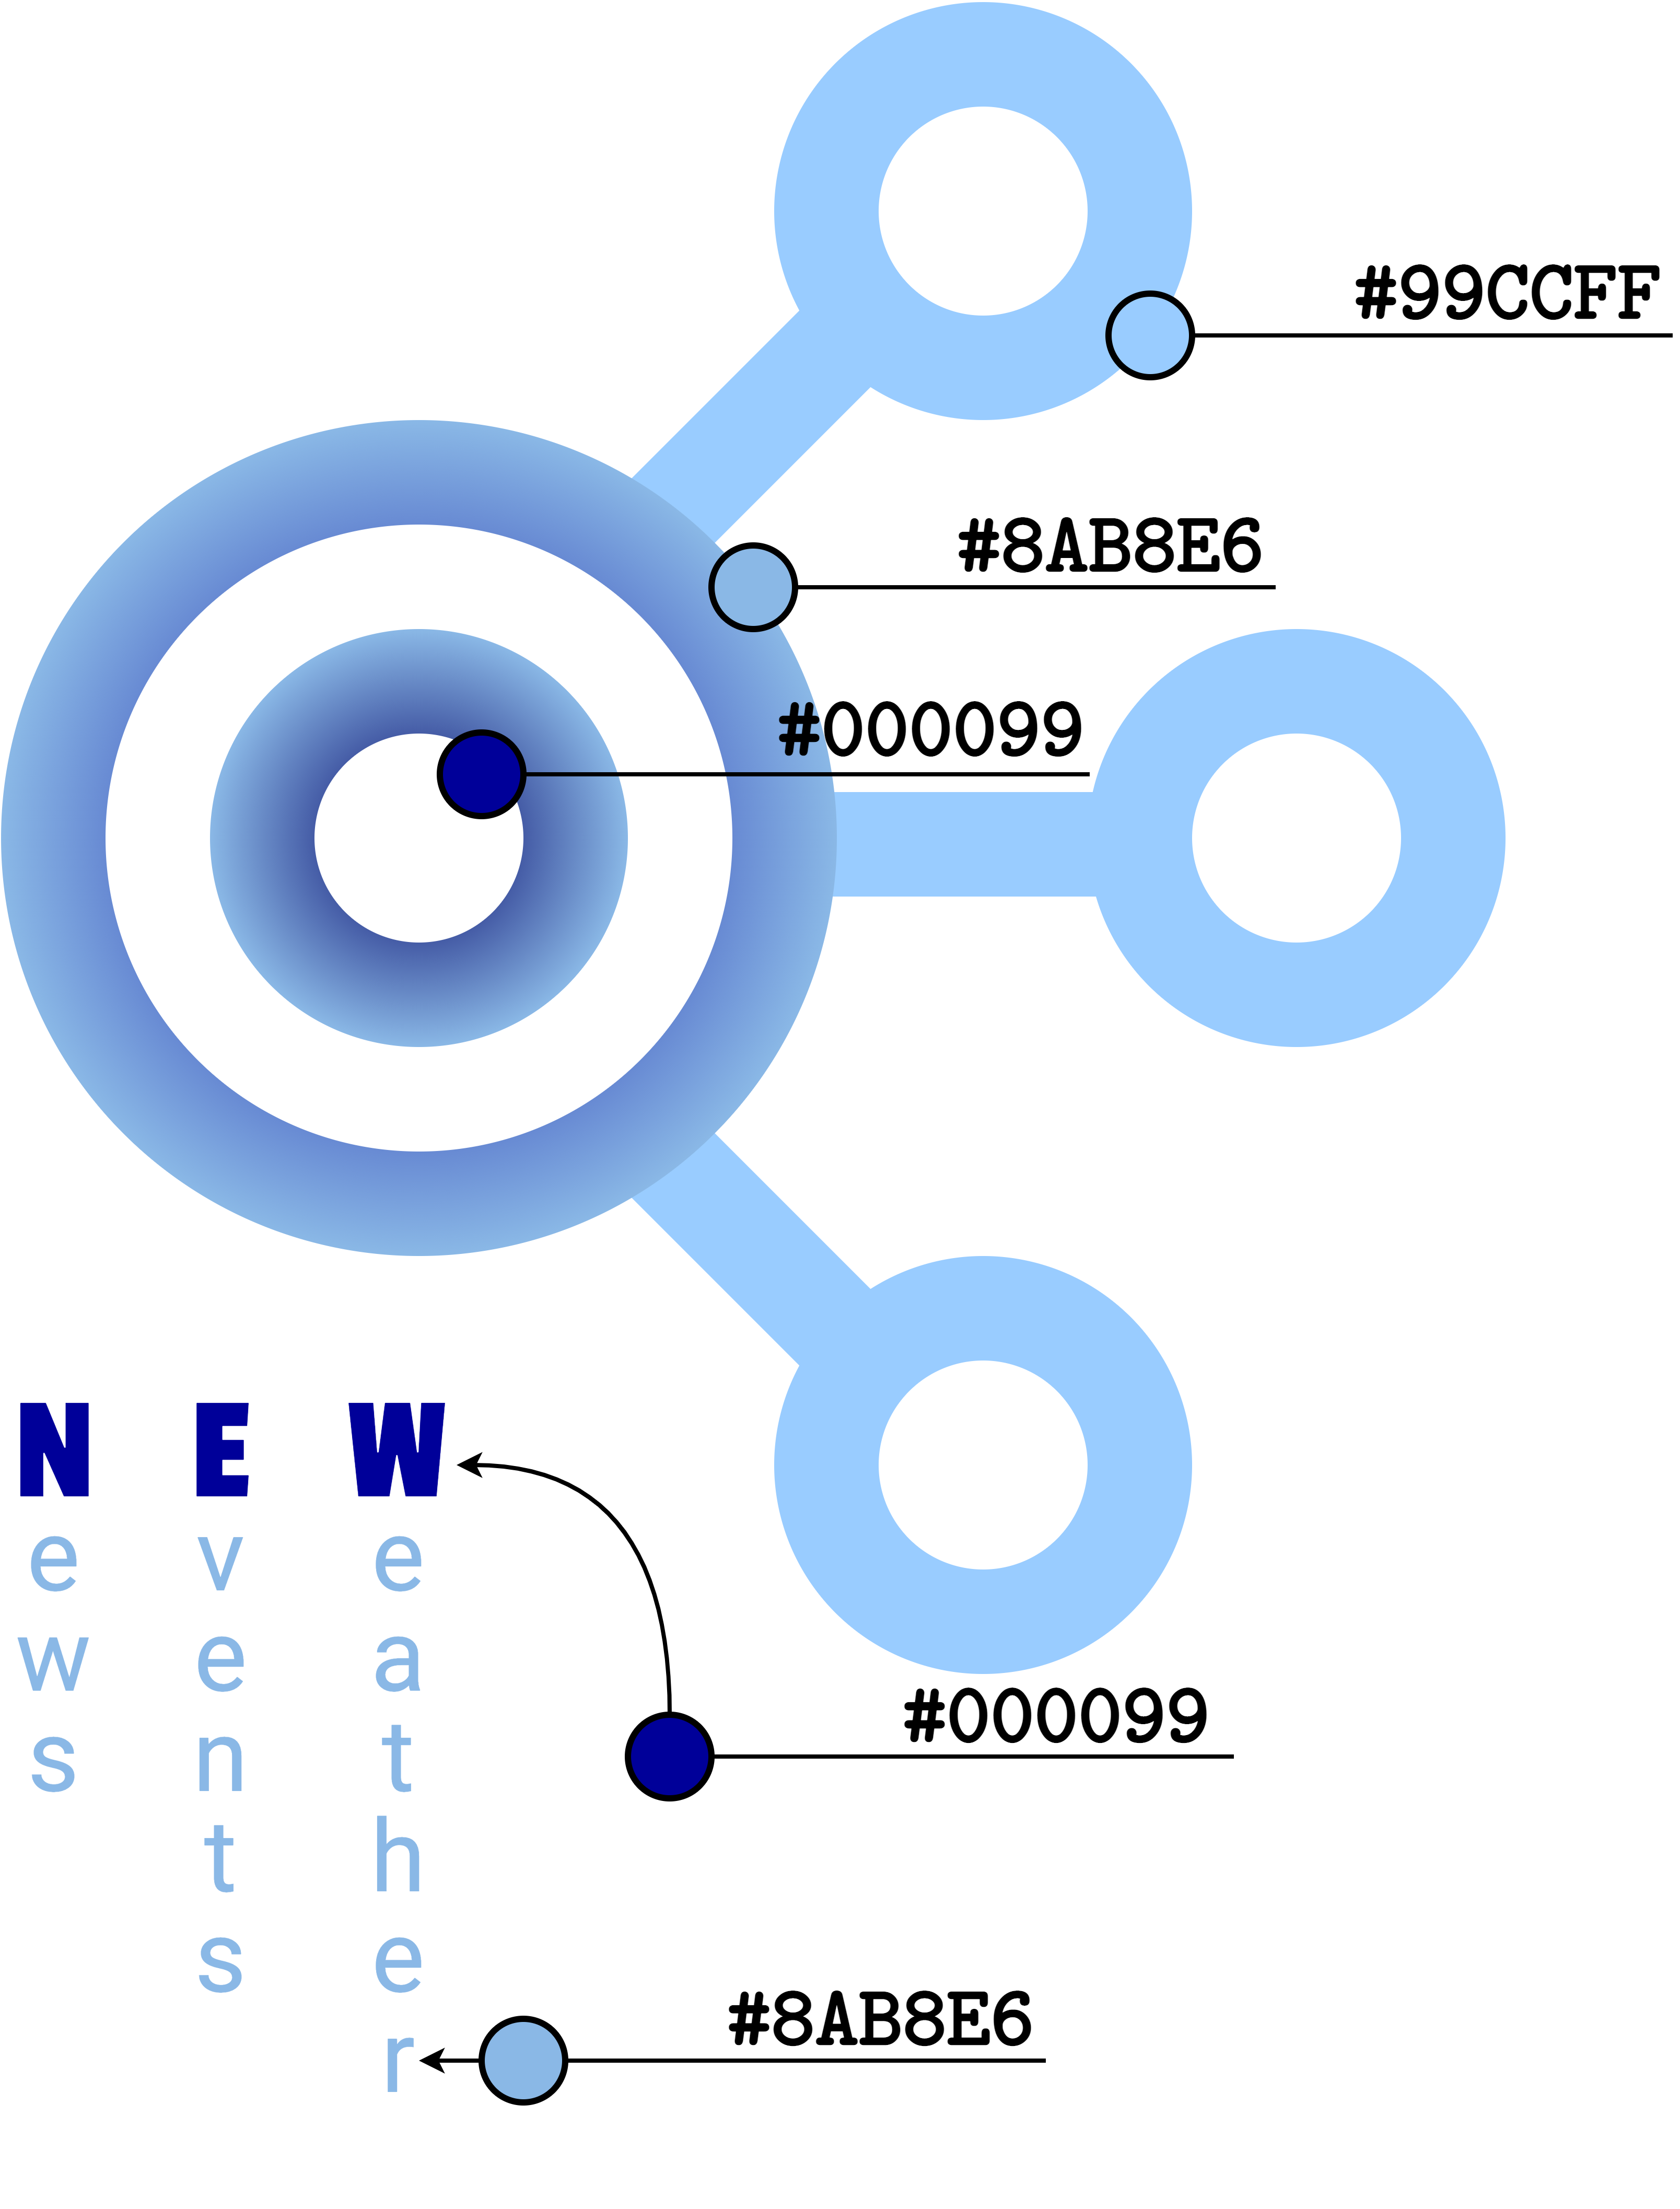
\includegraphics[scale=0.09]{images/LogoCromatico.png}
                                \end{center}
                                \caption{Composición cromática del logotipo}
                            \end{figure}

                            \newpage
                    
                            Tal y como se puede apreciar en la figura anterior, el logotipo tiene únicamente tres tonalidades de azúl. Azúl claro (\texttt{HEX 99CCFF}) para la silueta de los nodos, círculos exteriores y nombres (a excepción de las letras capitales), y un rango de degradado (\texttt{HEX 8AB8E6} $\rightarrow$ \texttt{000099}) para la figura central.\\

                            A partir de la selección de colores del logotipo, elaboramos una paleta de colores similares, para empezara trabajar con el diseño web de cara al usuario final.\\

                            Sacamos un total de 6 colores para la interfaz (elementos gráficos) y un total de 4 colores para tipografías.\\

                            \begin{center}
                                \underline{\textbf{Paleta de colores: elementos gráficos}}
                            \end{center}

                            \begin{figure}[H]
                                \begin{center}
                                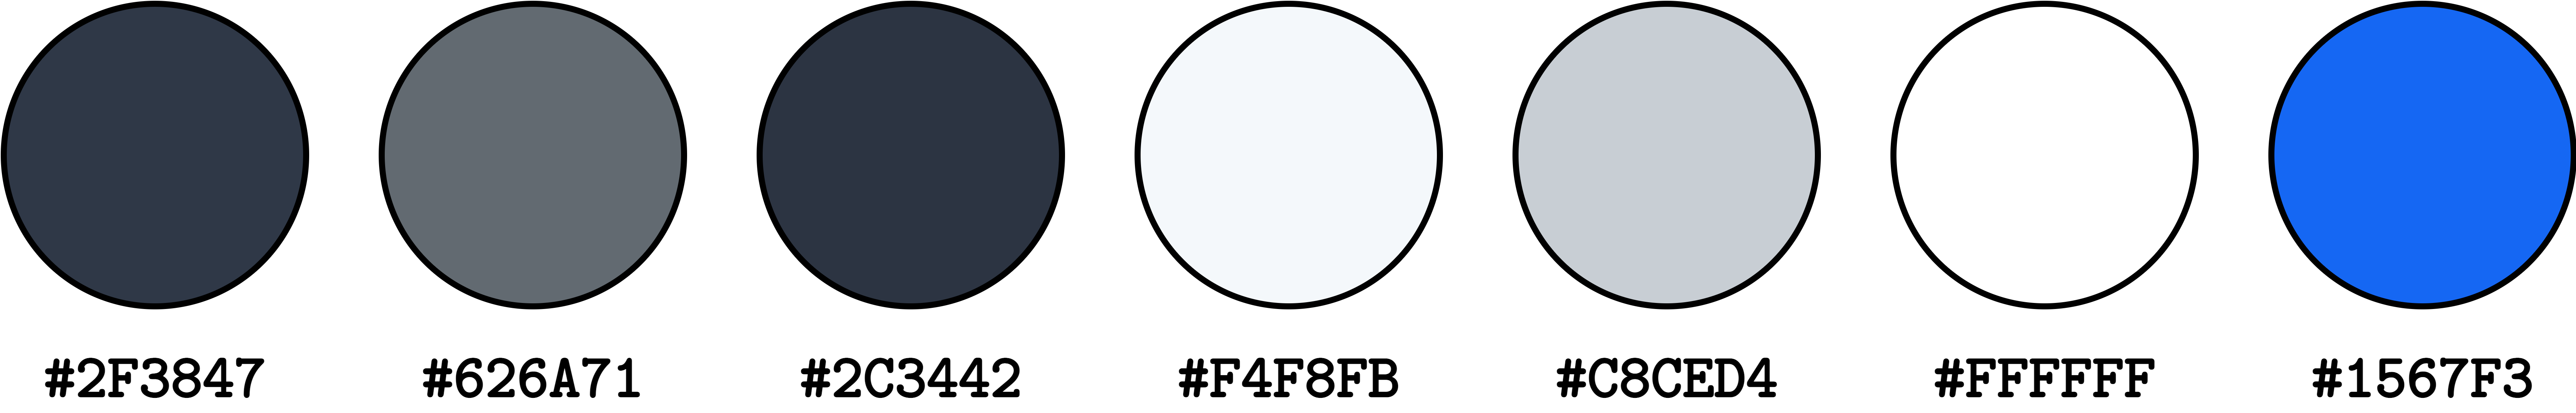
\includegraphics[scale=0.065]{images/ColorTyposNoTable.png}
                                \end{center}
                                \caption{Composición cromática de los elementos gráficos de la interfaz web}
                            \end{figure}

                            \vspace{5mm}
                            \begin{center}
                                \underline{\textbf{Paleta de colores: elementos tipográficos}}
                            \end{center}

                            \begin{figure}[H]
                                \begin{center}
                                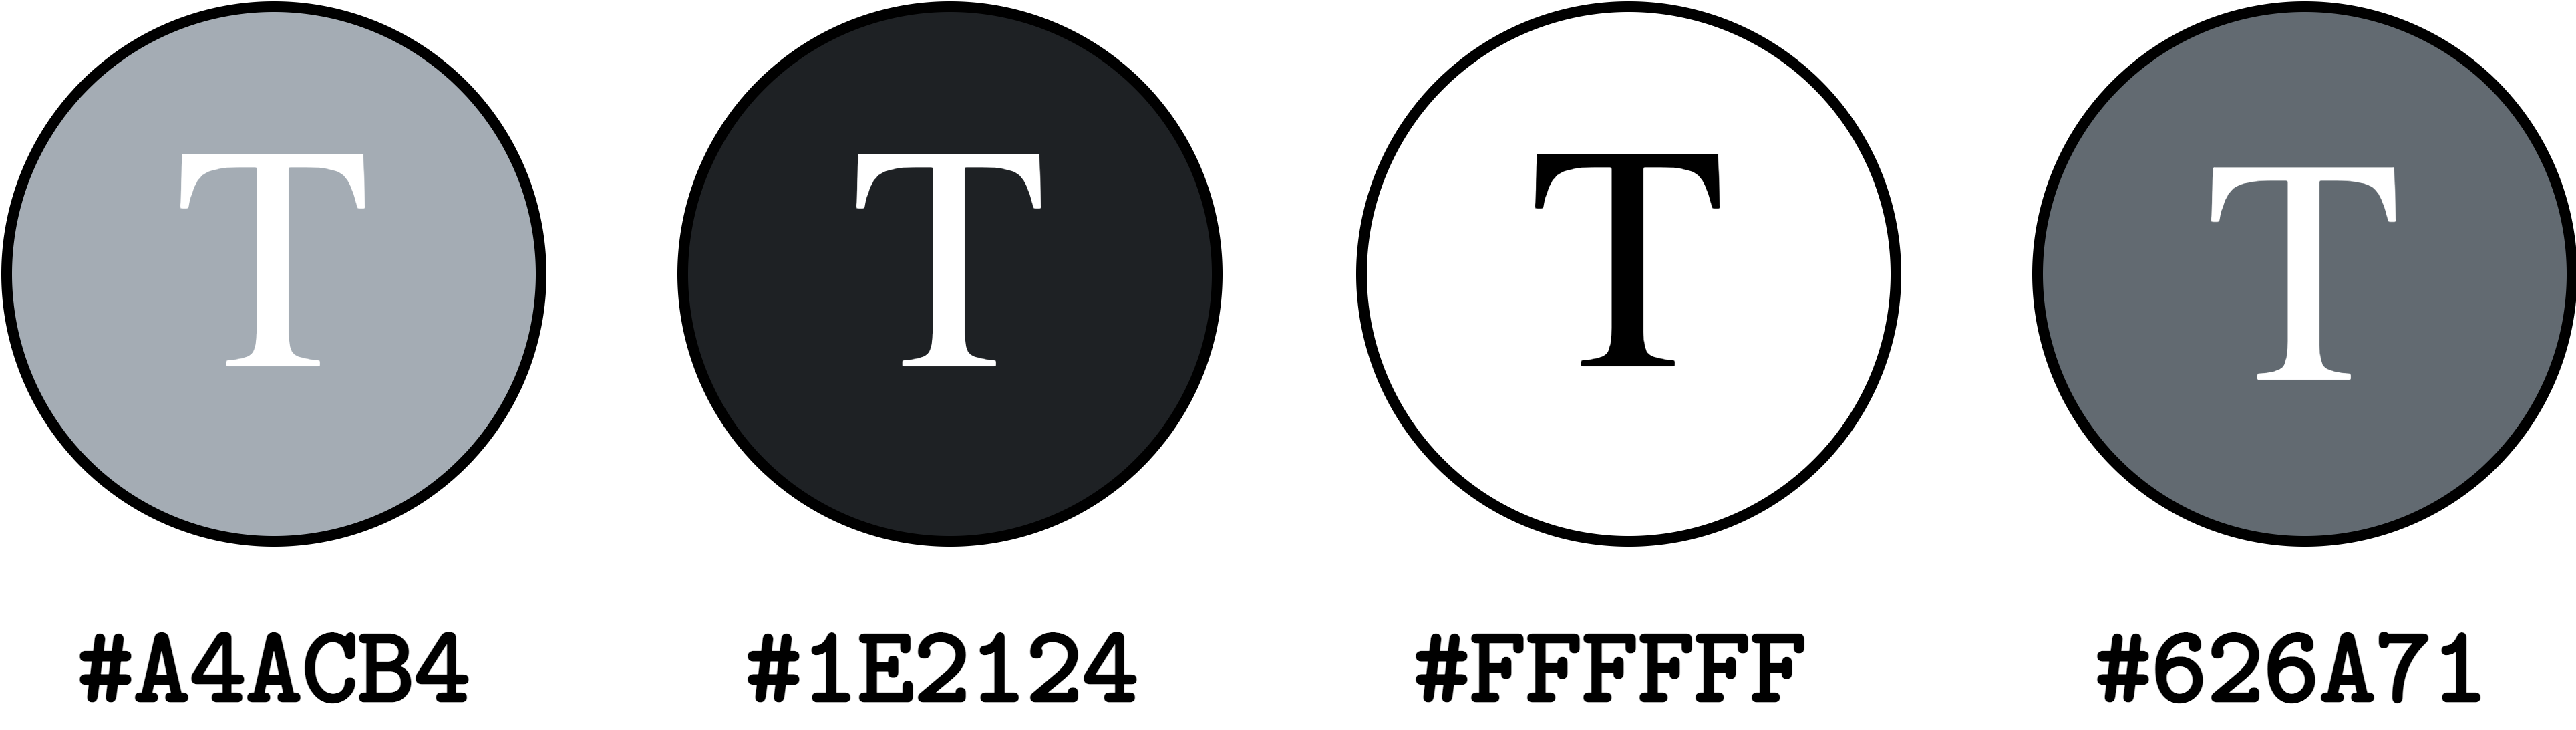
\includegraphics[scale=0.065]{images/ColorTypos2NoTable.png}
                                \end{center}
                                \caption{Composición cromática de las tipografías de la interfaz web}
                            \end{figure}
                            \vspace{5mm}


                            Teniendo en cuenta las paletas de colores anteriores, a la hora de hacer el diseño web, los colores de los elementos que se van a implementar, en todas las interfaces van a ser como la figura que sigue:

                            \newpage

                            \begin{center}
                                \underline{\textbf{Composición cromática de la página web}}
                            \end{center}

                            \begin{figure}[H]
                                \begin{center}
                                    \hspace*{-10mm}
                                \includegraphics[scale=0.057]{images/ColorWebInterfaceGeneral.png}
                                \end{center}
                                \caption{Composición cromática de la interfaz web}
                            \end{figure}

                    

                    
                            \paragraph{Tipografía}
                            La tipografía se define como el arte y la técnica en el manejo y selección de fuentes con el objetivo de crear trabajos de impresión. Por tanto, es un estilo visual con el que podemos dotar al contenido escrito que, si está bien elegido, ayudará a la lectura y dotará de armonía visual al concepto que queremos dar a conocer.\\
                    
                            Con el objetivo de elegir con éxito un conjunto de tipografías para el proyecto, en primer lugar, debemos tener en cuenta el \textit{target} al que va dirigido y su disponibilidad de caracteres:
                            
                                \begin{enumerate}
                                    \item \textbf{Objetivo y público}: Es preciso conocer de antemano el contexto del documento que vamos a tratar, ya sea un documento o aplicativo para un \textit{target} con cierto grado de especialización o un documento para todo tipo de públicos. En este caso, nuestra aplicación va a ser para todos los públicos, pero de caracter formal, por lo que debemos evitar tipografías con excesivo detalle o que se dificulte su lectura. También, teniendo en cuenta que la aplicación va a ser ejecutada y \textit{leída} en dispositivos móviles, evitaremos el uso de tipografías estilo \textit{Serif}.
                                    \item \textbf{Disponibilidad de caracteres}: La tipografía a utilizar debe poseer todas y cada una de las grafías necesarias para el idioma en el que se va a utilizar, y en este caso también debe soportar caracteres especiales \textit{ASCII}. Podemos complementar la tipografía utilizada con iconos especiales de \textit{Google Fonts} o de bibliotecas especiales de \textit{Bootstrap}.
                                \end{enumerate}
                    
                            \paragraph*{Documento escrito o memoria del proyecto}
                            Teniendo en cuenta los puntos anteriores, directamente hemos implementado todo el contenido de la memoria en un editor de texto en lenguaje \LaTeX, por el hecho de que hay fragmentos de esta memoria (a diferencia de su implementación web) que contienen información técnica, fragmentos de código y otros elementos en los que el uso de \LaTeX son una clara ventaja a tener en cuenta.\\
                    
                            Las tipografías que se utilizan en este documento son de la familia \texttt{Modern Roman} (a 11 puntos de tamaño y en \texttt{\textbackslash normalsize}):
                                \begin{itemize}
                                    \item \textbf{Latin Modern Roman}: De ahora en adelante LMR, se trata de una fuente tipo \textit{serif}, creada por \textit{GUST e-foundry} y cuenta con 12 estilos. Es la fuente predeterminada de \LaTeX para el texto general en la clase \texttt{article}. Los estilos que utiliza esta tipogrrafía son los siguientes:
                                        \begin{itemize}
                                            \item \textbf{LMR Regular}: Utilizada para el texto en general.
                                            \begin{figure}[H]
                                                \begin{center}
                                                \fbox{
\includegraphics[scale=0.30]{fonts/LMRRegular.png}}
                                                \end{center}
                                            \end{figure}
                    
                                            \item \textbf{LMR Italic}: Utilizada para las secciones de texto en cursiva.
                                            \begin{figure}[H]
                                                \begin{center}
                                                \fbox{
\includegraphics[scale=0.30]{fonts/LMRItalic.png}}
                                                \end{center}
                                            \end{figure}

                                            \newpage
                    
                                            \item \textbf{LMR Bold}: Utilizada para las secciones de texto en negrita.
                                            \begin{figure}[H]
                                                \begin{center}
                                                \fbox{
\includegraphics[scale=0.30]{fonts/LMRBold.png}}
                                                \end{center}
                                            \end{figure}
                                        \end{itemize}
                                    \item \textbf{Latin Modern Mono}: De ahora en adelante LMM, se trata de una fuente monoespaciada\footnote{\textbf{Tipografía monoespaciada}: es aquella en la que todos sus caracteres ocupan el mismo espacio horizontal.} creada por \textit{GUST e-foundry}, de tipo \textit{serif} que cuenta con 17 estilos.Es la fuente predeterminada por \LaTeX para mostrar contenido de código fuente. Aunque esta tipografía cuenta con muchas variantes, en este documento únicamente se ha utilizado la variante \textit{Regular}, y para resaltar la sintaxis se ha utilizado un código de colores (naranja = \textit{strings}, azul = palabras reservadas, gris = comentarios y negro = resto del código).
                                        \begin{itemize}
                                            \item \textbf{LMM Regular}: Utilizada para las secciones de código fuente.
                                            \begin{figure}[H]
                                                \begin{center}
                                                \fbox{
\includegraphics[scale=0.30]{fonts/LMMRegular.png}}
                                                \end{center}
                                            \end{figure}
                                        \end{itemize}                
                                \end{itemize}
                                El resto de tipografías que aparecen en este documento (figuras o esquemas), provienen de imágenes insertadas en formato \texttt{.png} (mapa de bits) o \texttt{.svg} (formato vectorial), por lo que su tipografía a expensas de ser material creado para tal fin (la edición de este documento) no ha podido ser editada y tratada.
                            
                                \paragraph*{Imagotipos prinicipal y secundario}
                                Cuidar y tener en cuenta el aspecto físico y tipográfico en el logotipo de la marca que queremos promocionar es de vital importancia porque esta será la seña de identidad tanto en la aplicación como en los documentos donde haga referencia a la misma. En nuestro caso, para el logotipo (imagotipo, es decir, con letra), hemos elegido dos tipografias para el texto. Una de ellas de realce y en mayúsculas: \textit{Passion One}, y la que hace referencia a las letras en minúscula, una tipografía mucho más fina: \textit{Roboto}.\\
                    
                                El uso de estas dos tipografías sin \textit{serifas}\footnote{\textbf{Serifa}: o gracia, es un trazo decorativo que forma la terminación de las astas de los caracteres de algunas tipografías.}, trata de dar un aspecto mucho más limpio, minimalista y moderno a los títulos del logotipo. La relación de proporción que guardan estas dos tipografías es de 72:48 puntos (ó 3:2) respectivamente \textit{Passion One}:\textit{Roboto}.
                    
                                \begin{itemize}
                                    \item \textbf{Passion One}: Se trata de una tipografía de tipo \textit{sans serif}, creada por \textit{Fontstage}, diseñada para impresiones de títulos a gran tamaño y cuenta con 3 estilos. Es una de las fuentes utilizadas para implementar el logotipo de nuestra marca. Hemos utilizado únicamente su estilo \textit{Regular}.
                                        \begin{itemize}
                                            \item \textbf{Passion One Regular}: Utilizada para los caracteres en mayúsculas del título de nuestro logotipo: '\textit{N E W}'.
                                            \begin{figure}[H]
                                                \begin{center}
                                                \fbox{
\includegraphics[scale=0.30]{fonts/PassionOneRegular.png}}
                                                \end{center}
                                            \end{figure}
                                        \end{itemize}
                                    \item \textbf{Roboto}: Se trata de una tipografía de tipo \textit{sans serif}, creada por \textit{Christian Robertson}, que cuenta con 18 estilos y fue diseñada principalmente para su uso en plataformas online debido a su gran facilidad de lectura. Es otra de las fuentes que hemos utilizado para las letras del logotipo de nuestra marca. Aunque, de sus muchos estilos, hemos utilizado únicamente su estilo \textit{Regular}.
                                        \begin{itemize}
                                            \item \textbf{Roboto Regular}: Utilizada para los caracteres en minúsculas del título de nuestro logotipo: '\textit{ews}, \textit{vents} y \textit{eather}'.
                                            \begin{figure}[H]
                                                \begin{center}
                                                \fbox{
\includegraphics[scale=0.30]{fonts/RobotoRegular.png}}
                                                \end{center}
                                            \end{figure}
                                        \end{itemize}
                                \end{itemize}

                                \paragraph*{Implementación de la aplicación}
                                Para la implementación de la aplicación, hemos decidido ir a una tipografía especializada en interfaces web, sobria y de muy fácil lectura. Se trata de \textit{Nunito Sans}, una tipografía \textit{Sans Serif} que podemos encontrar en la biblioteca de \textit{Google Fonts}, por lo que nos aseguramos que con cualquier navegador moderno, será legible para todo tipo de usuarios.\\
                        
                                Las tipografías que se utilizan en la implementación web son de la familia \texttt{Nunito Sans} (de tamaño variable) y según su contexto, en modo normal o negrita:
                                \newpage
                                    \begin{itemize}
                                        \item \textbf{Nunito Sans}: Es trata una fuente tipo \textit{serif}, creada por \textit{Jacques Le Bailly} y cuenta con 14 estilos. Los estilos que utiliza esta tipografía son dos:
                                            \begin{itemize}
                                                \item \textbf{Nunito Sans Regular}: Utilizada para el texto en general.
                                                \begin{figure}[H]
                                                    \begin{center}
                                                    \fbox{
\includegraphics[scale=0.30]{fonts/NunitoSansRegular.png}}
                                                    \end{center}
                                                \end{figure}
                        
                                                \item \textbf{Nunito Sans Bold}: Utilizada títulos y encabezamientos se secciones.
                                                \begin{figure}[H]
                                                    \begin{center}
                                                    \fbox{
\includegraphics[scale=0.30]{fonts/NunitoSansBold.png}}
                                                    \end{center}
                                                \end{figure}
                                            \end{itemize}
                                        \end{itemize}



                                \newpage
                                \subsubsection{Interfaz de usuario}
                                    \paragraph{Bosquejo inicial}
                                A continuación y de forma muy simple, adjuntamos dos \textit{mockups}, es decir, dos diseños preliminares de la interfaz de usuario que tendrá la aplicación. Se trata de una aplicación web y por tanto, puede ser accesible desde cualquier dispositivo. Se muestra con esquema de colores claro y oscuro.
                                \begin{figure}[H]
                                    \begin{center}
                                    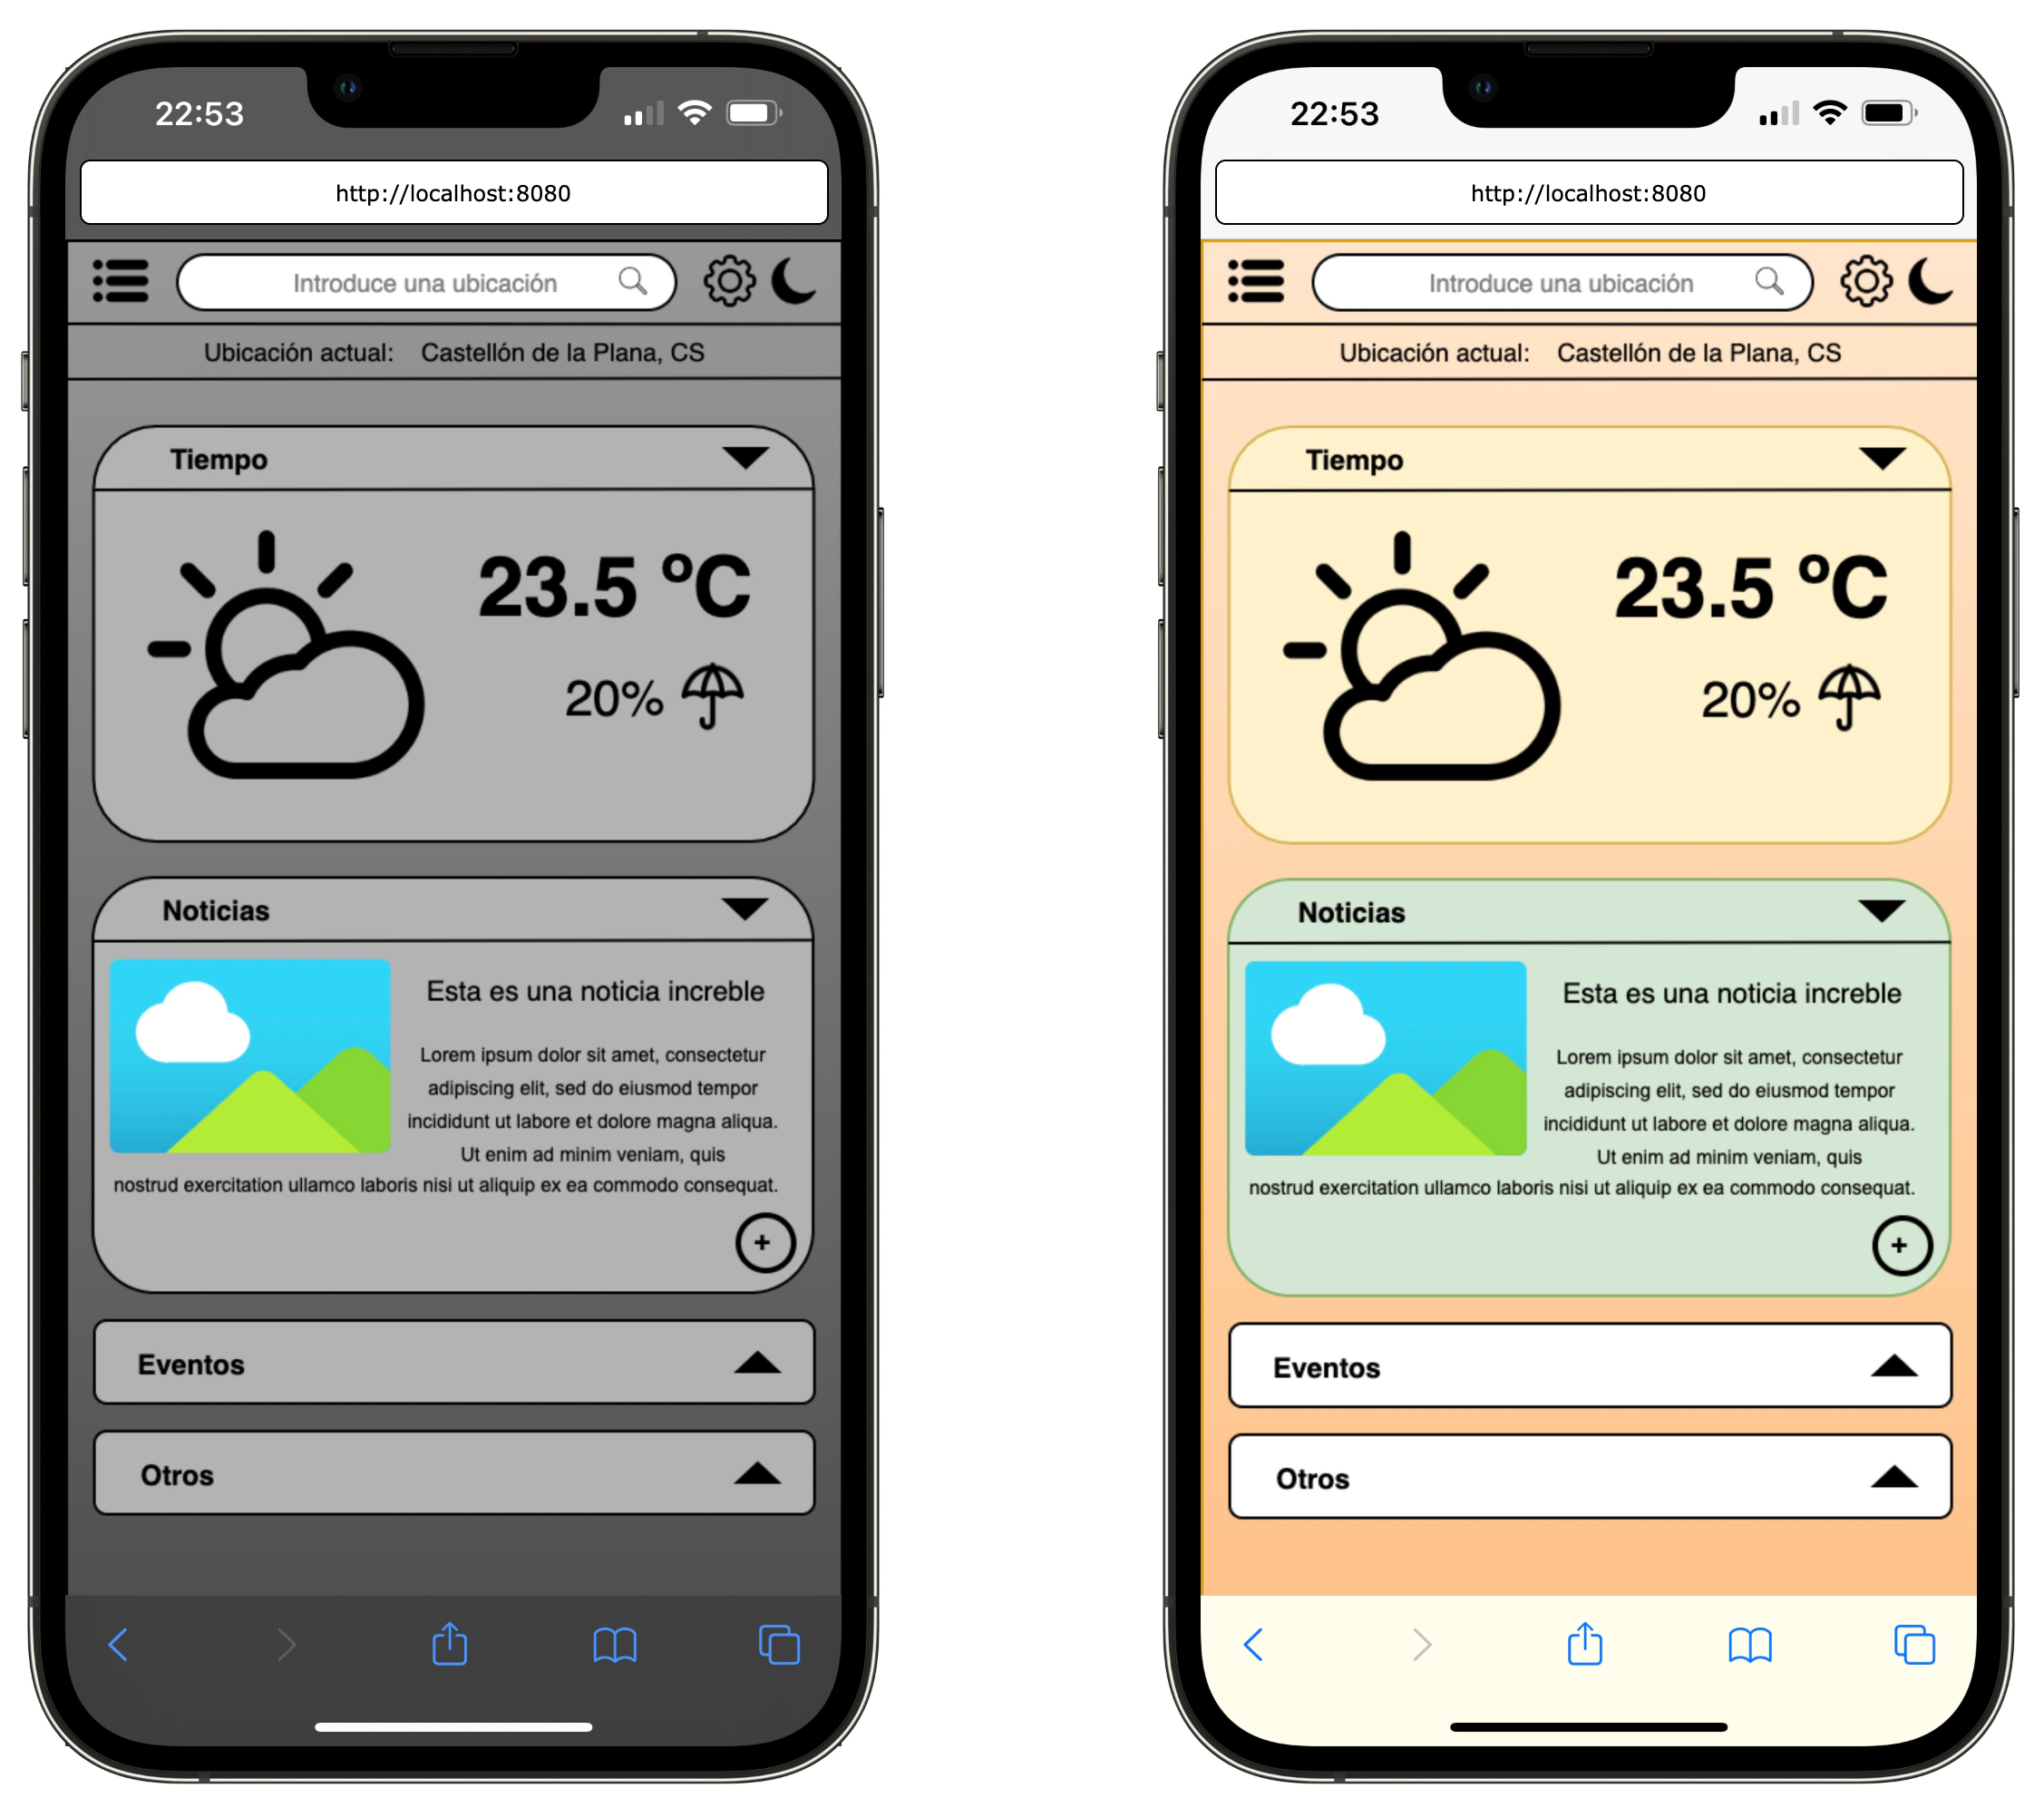
\includegraphics[scale=0.18]{images/GuiTelefono.png}
                                    \end{center}
                                    \caption{Propuesta de la GUI con dos esquemas de colores}
                                \end{figure}
                                A modo de esquema, estas son algunas características que estarán disponibles en la versión final funcional (aunque estas características pueden variar de cara a la entrega final):
                        
                                \begin{itemize}
                                    \item Botones triangulares para expandir las tarjetas de información, y así poder mostrar u ocultar información relevante.
                                    \item Al menos dos esquemas de colores diferenciados. Uno para el día y otro para la noche (o situaciones de baja iluminación). Para acceder a este ajuste, podremos pulsar una media luna en la parte superior derecha.
                                    \item La app nos permitirá cambiar desde Ajustes algunos valores de la misma, así como desactivar servicios API para que no aparezcan en el \textit{dashboard} principal.
                                    \item Si no existe información via API de un lugar, esa tarjeta no se mostrará.
                                    \item Algunas de las tarjetas serán clickables y permitirán algún tipo de interacción con ellas.
                                \end{itemize}

                                Finalmente, a lo largo del proyecto, valoramos cuales de los anteriores puntos son cruciales en el diseño y cuales son secundarios. Para futuras implementaciones, si se diese el caso, implementaríamos el modo noche, y diferentes esquemas de colores a configuración del usuario.


                                \paragraph{Bosquejo de alta fidelidad}
                                Con la finalidad de implementar un modelo de alta calidad, recurrimos a herraminetas profesionales (\textit{Justinmind}) para hacer un bosquejo de alta fidelidad. En este bosquejo, tenemos en cuenta las proporciones del layout a implementar, y en un iniciio, proponemos un sistema de información via tarjetas (como \textit{Google Discovery}). El bosquejo siguiente es el primero que realizamos de alta fidelidad:

                                \begin{figure}[H]
                                    \begin{center}
                                        \hspace*{-7mm}
                                    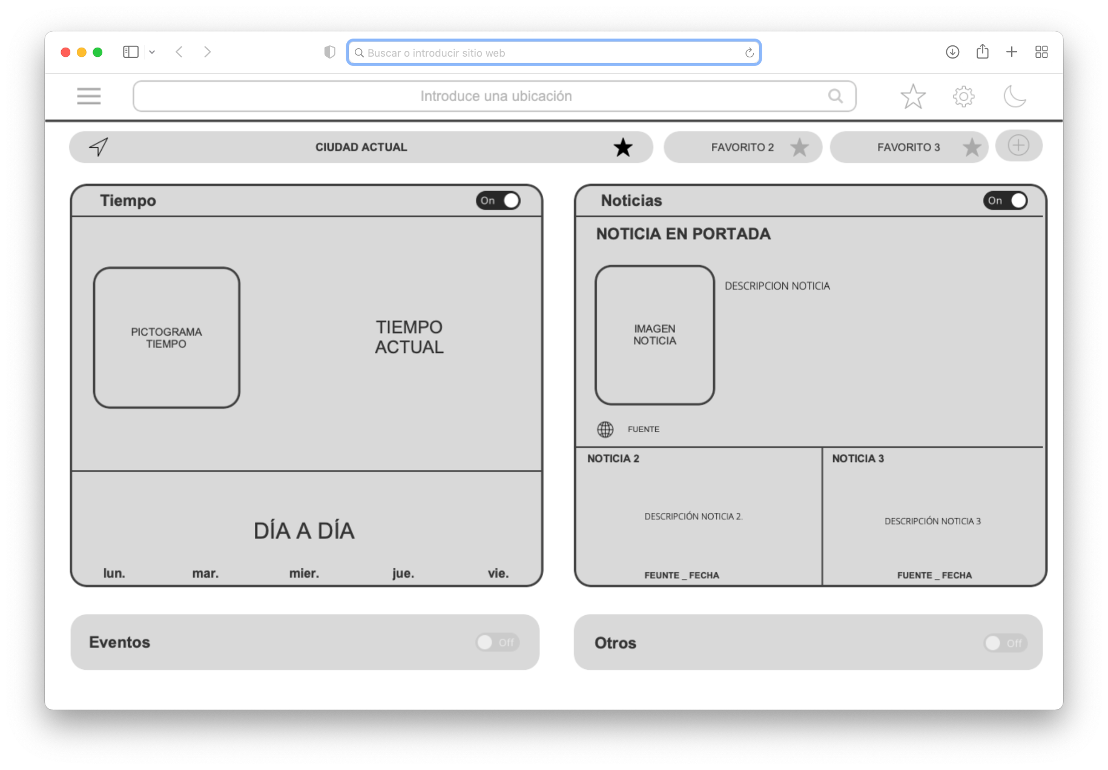
\includegraphics[scale=0.87]{images/Boceto1.png}
                                    \end{center}
                                    \caption{Bosquejo de alta fidelidad inicial}
                                \end{figure}

                                En el bosquejo anterior, podemos observar como el layout se ha dividido horizontalmente en 2 secciones, y 2 tarjetas en cada una de ellas.\\
                                
                                En el momento que hacemos este bosquejo, aún no hemos empezado con el diseño gráfico de la aplicación, por lo que el tener una leve idea de como vamos a organizar los elementos en pantalla, el tamaño de las fuentes tipográficas, etc. Todos los bosquejos que se realizan tienen un tamaño de layout de \texttt{1280x800} píxeles.\\

                                A partir del bosquejo anterior, añadimos texto y color, para valorar diferentes paletas cromáticas.\\

                                \begin{center}
                                    \underline{\textbf{UI: Clara}}
                                \end{center}

                                \begin{figure}[H]
                                    \begin{center}
                                        \hspace*{-7mm}
                                    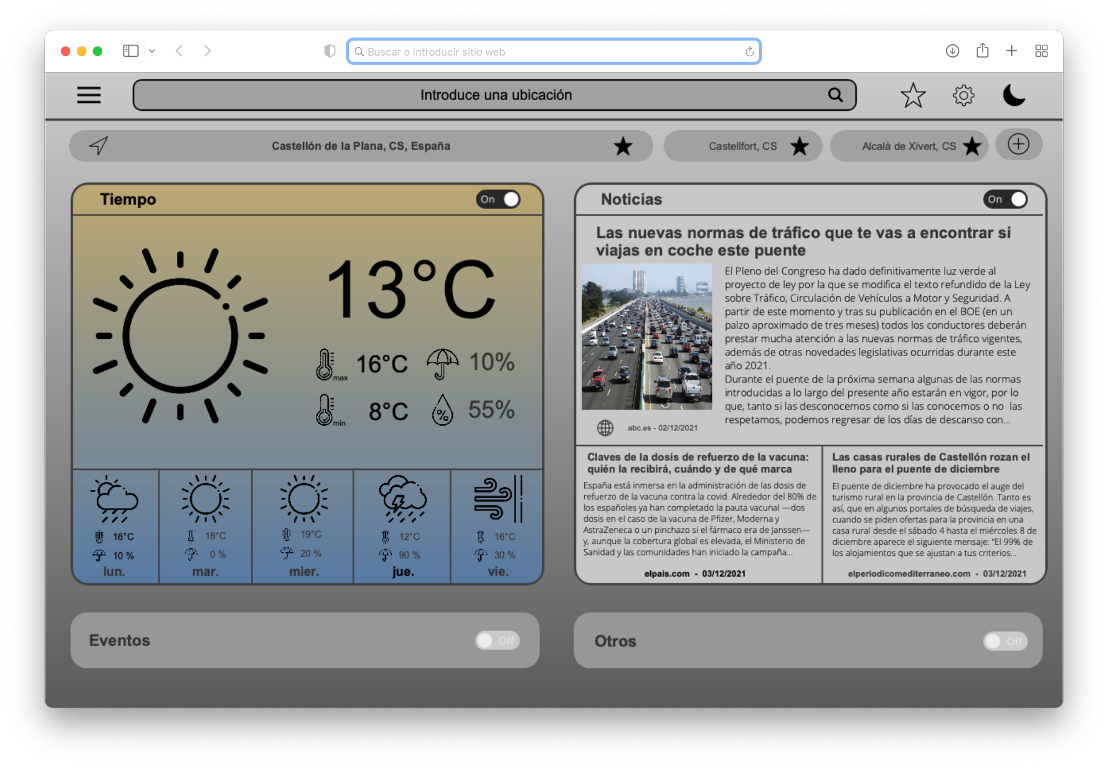
\includegraphics[scale=0.861]{images/Boceto2.png}
                                    \end{center}
                                    \caption{Propuesta de alta fidelidad en esquema de color claro}
                                \end{figure}

                                Valoramos también un esquema de colores oscuros, aunque finalmente decidimos apostar por un modo único de representación cromática.

                                \newpage

                                \begin{center}
                                    \underline{\textbf{UI: Oscura}}
                                \end{center}


                                \begin{figure}[H]
                                    \begin{center}
                                        \hspace*{-5mm}
                                    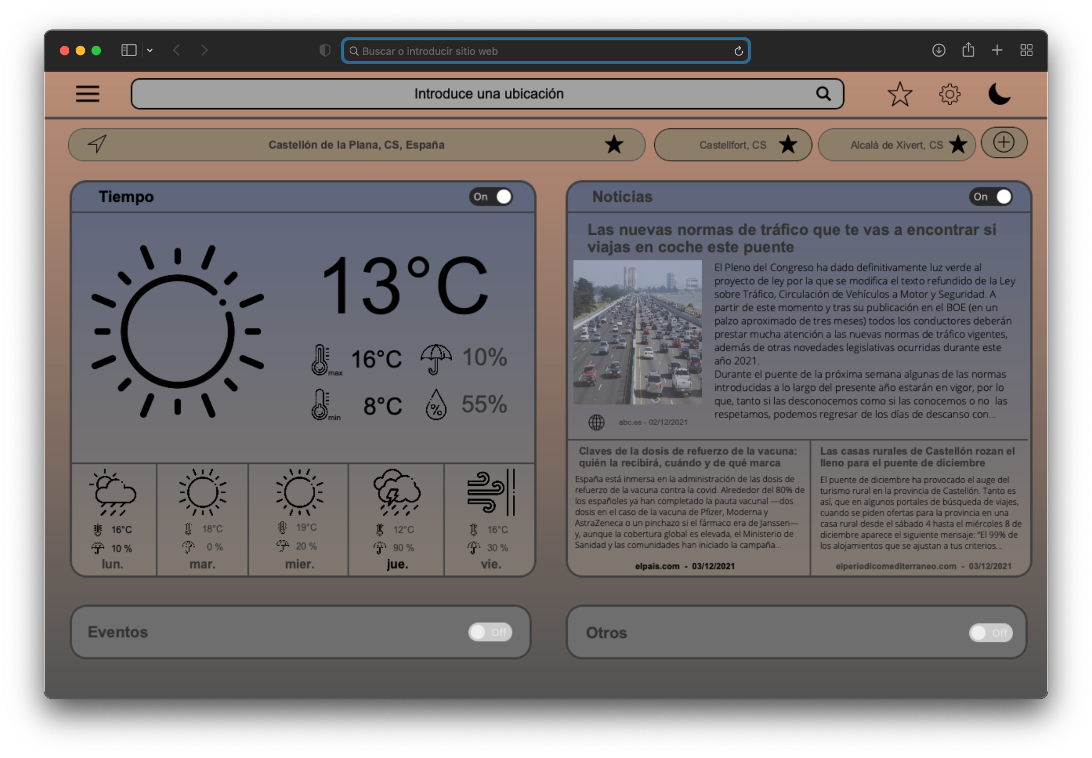
\includegraphics[scale=0.87]{images/Boceto3.png}
                                    \end{center}
                                    \caption{Propuesta de alta fidelidad en esquema de color oscuro}
                                \end{figure}


                                Teniendo en cuenta que nos basamos en el esquema de colores del punto \texttt{4.5.1.4} en la paleta de colores del logotipo, preparamos un nuevo layout con un panel de ajustes.

                                \newpage
                                \begin{center}
                                    \underline{\textbf{UI: Clara + Opciones}}
                                \end{center}

                                \vspace*{-5mm}
                                \begin{figure}[H]
                                    \begin{center}
                                        \hspace*{-8mm}
                                    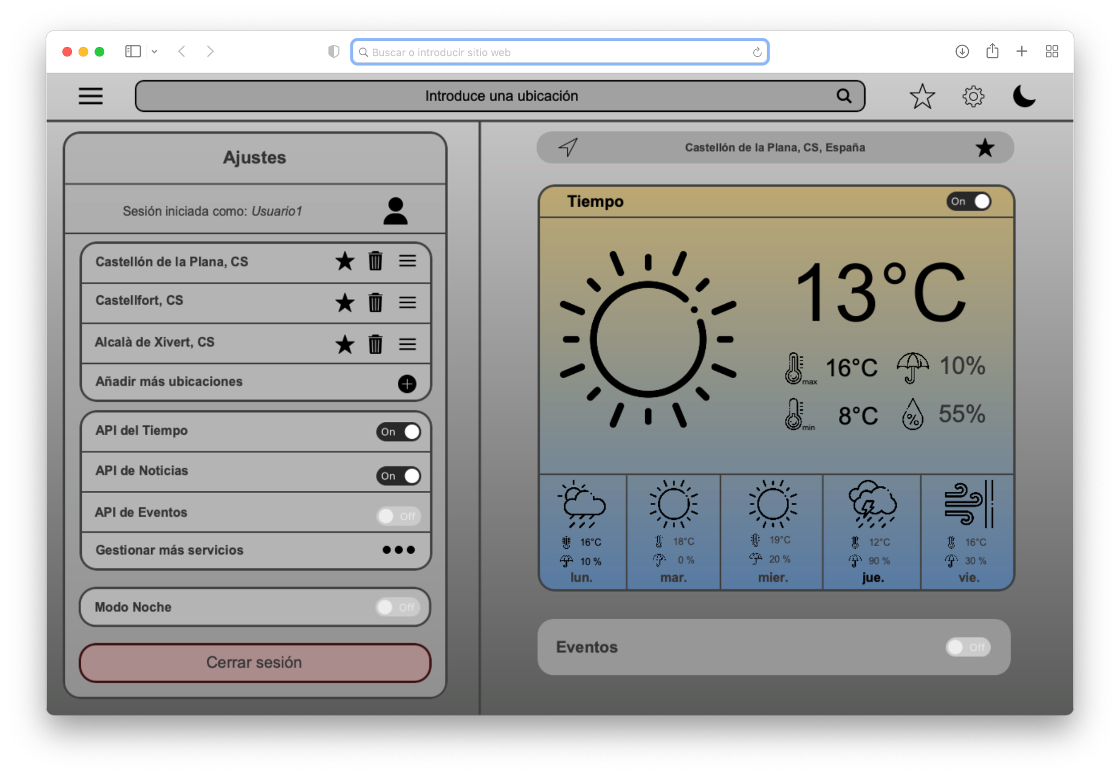
\includegraphics[scale=0.867]{images/Boceto4.png}
                                    \end{center}
                                    \caption{Propuesta de alta fidelidad en con panel de ajustes lateral}
                                \end{figure}

                                Este último bosquejo recoge en un panel lateral una serie de ajustes que vamos a implementar: guardar ubicación como favorito, activar o descativar apis y conectarse como usuario y desconectarse.\\

                                \paragraph{Implementación real}

                                Despues de dos iteraciones de bosquejos, implementamos ya la herramienta real. Esta implementación utiliza \textbf{React} con la paleta de colores vista en el punto \texttt{4.5.1.4} y un diseño límpio y minimalista.\\

                                En primer lugar, cuando iniciamos el servicio, se nos redirigirá a la página web por defecto: \texttt{localhost:8080}.\\


                                \begin{figure}[H]
                                    \begin{center}
                                        \hspace*{-7mm}
                                    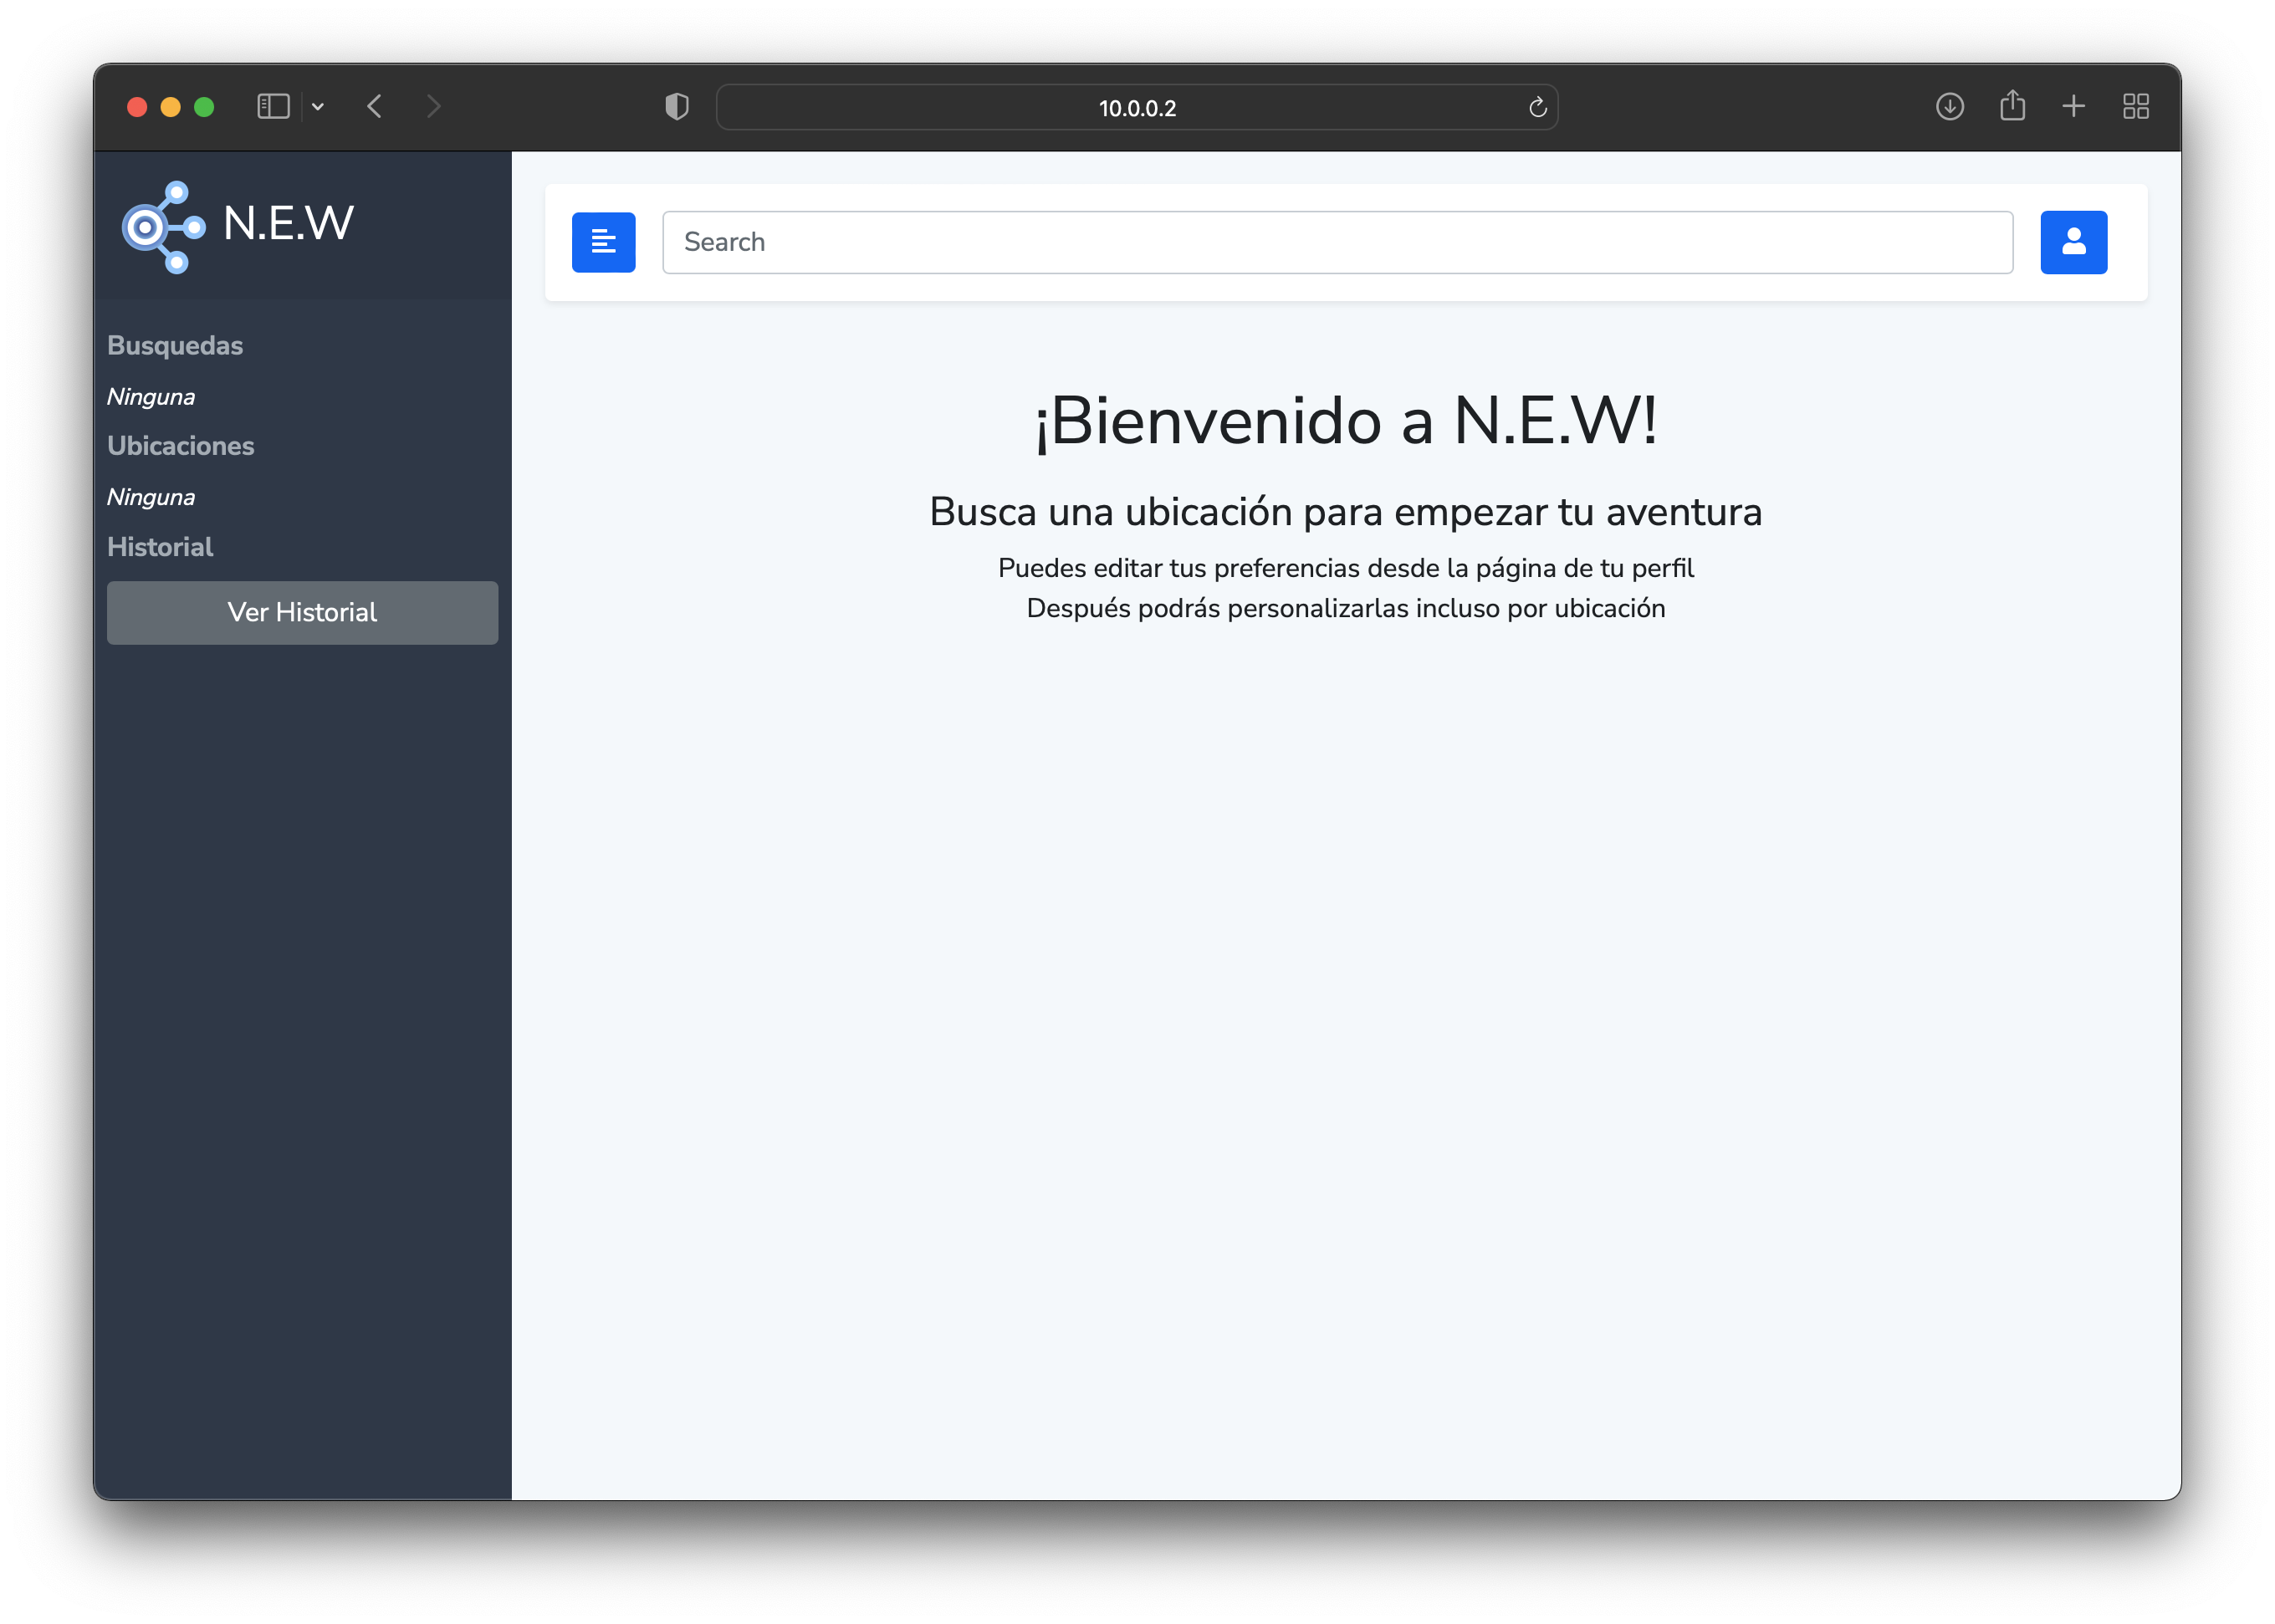
\includegraphics[scale=0.342]{images/final1.png}
                                    \end{center}
                                \end{figure}

                                \vspace*{-5mm}
                                Podemos registrarnos o iniciar sesión (si previamente hemos creado una cuenta) dando click al icono usuario en la parte superior derecha de la pantalla.
                                \vspace*{-2mm}

                                \begin{figure}[H]
                                    \begin{center}
                                        \hspace*{-7mm}
                                    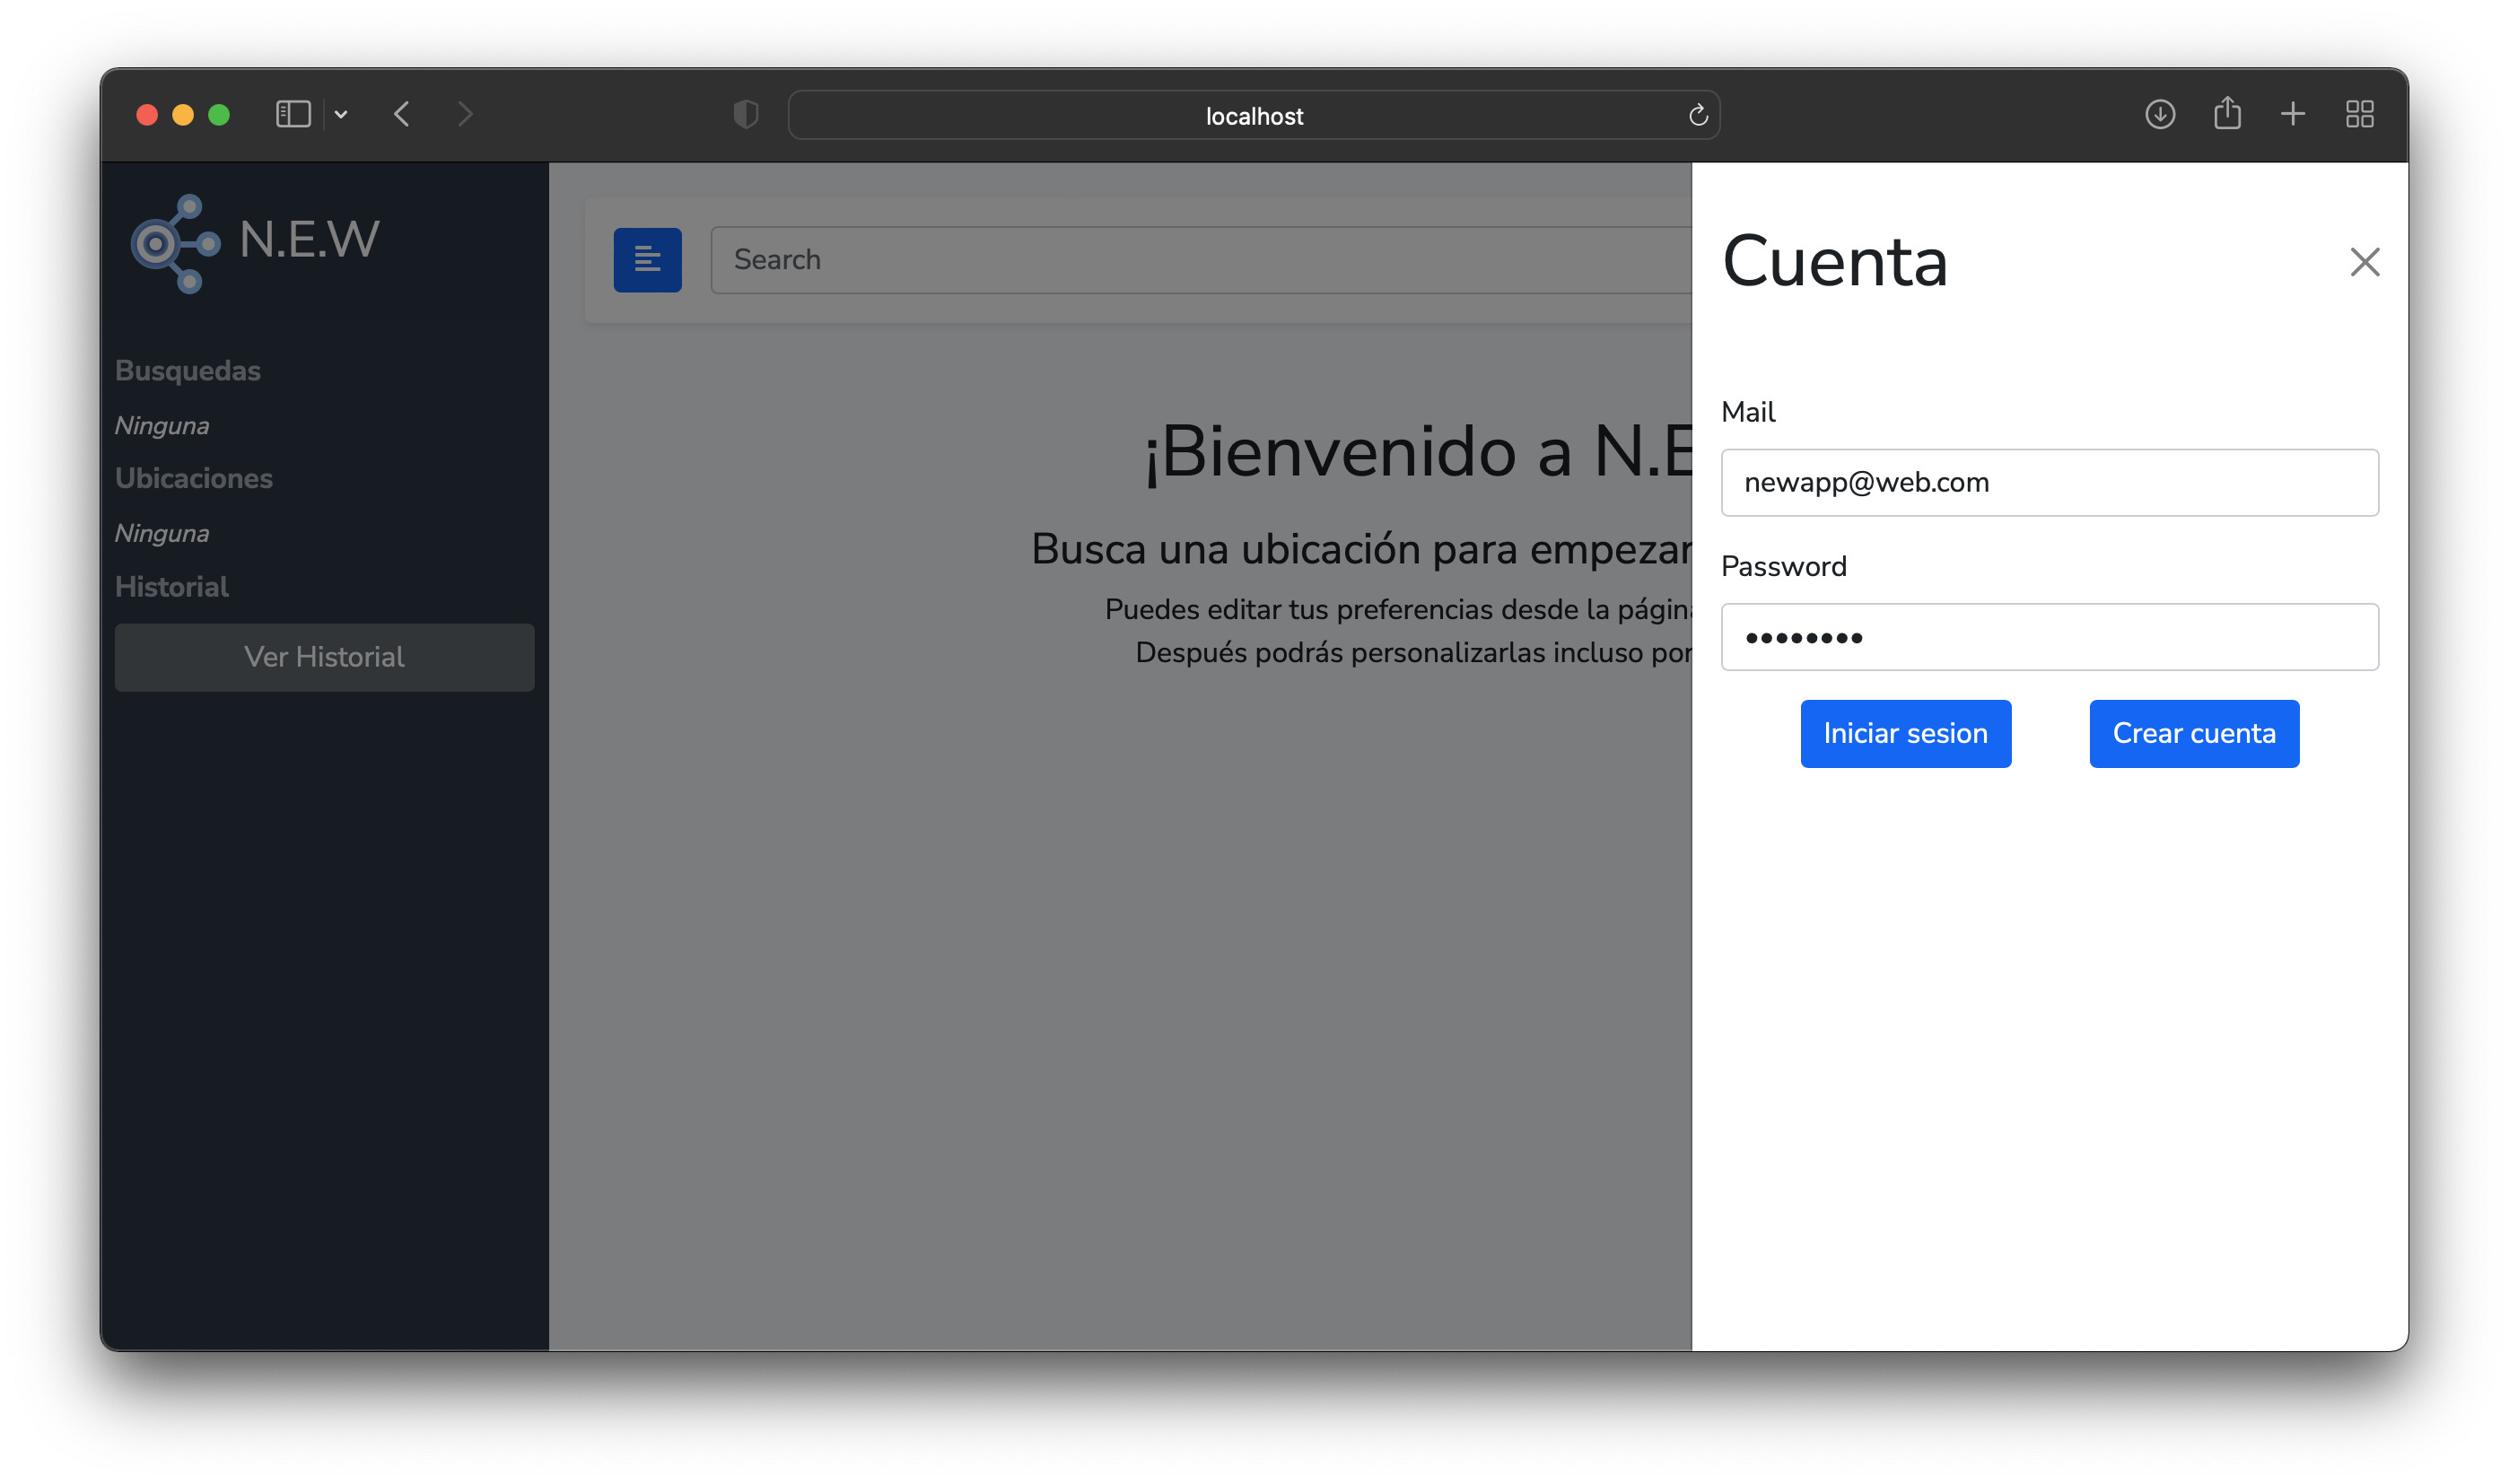
\includegraphics[scale=0.342]{images/final2.png}
                                    \end{center}
                                \end{figure}

                                Una vez nos hemos logueado, podemos activar o desactivar servicios API para ver a posteriori información relacionada con estos ítems.



                                \begin{figure}[H]
                                    \begin{center}
                                        \hspace*{-7mm}
                                    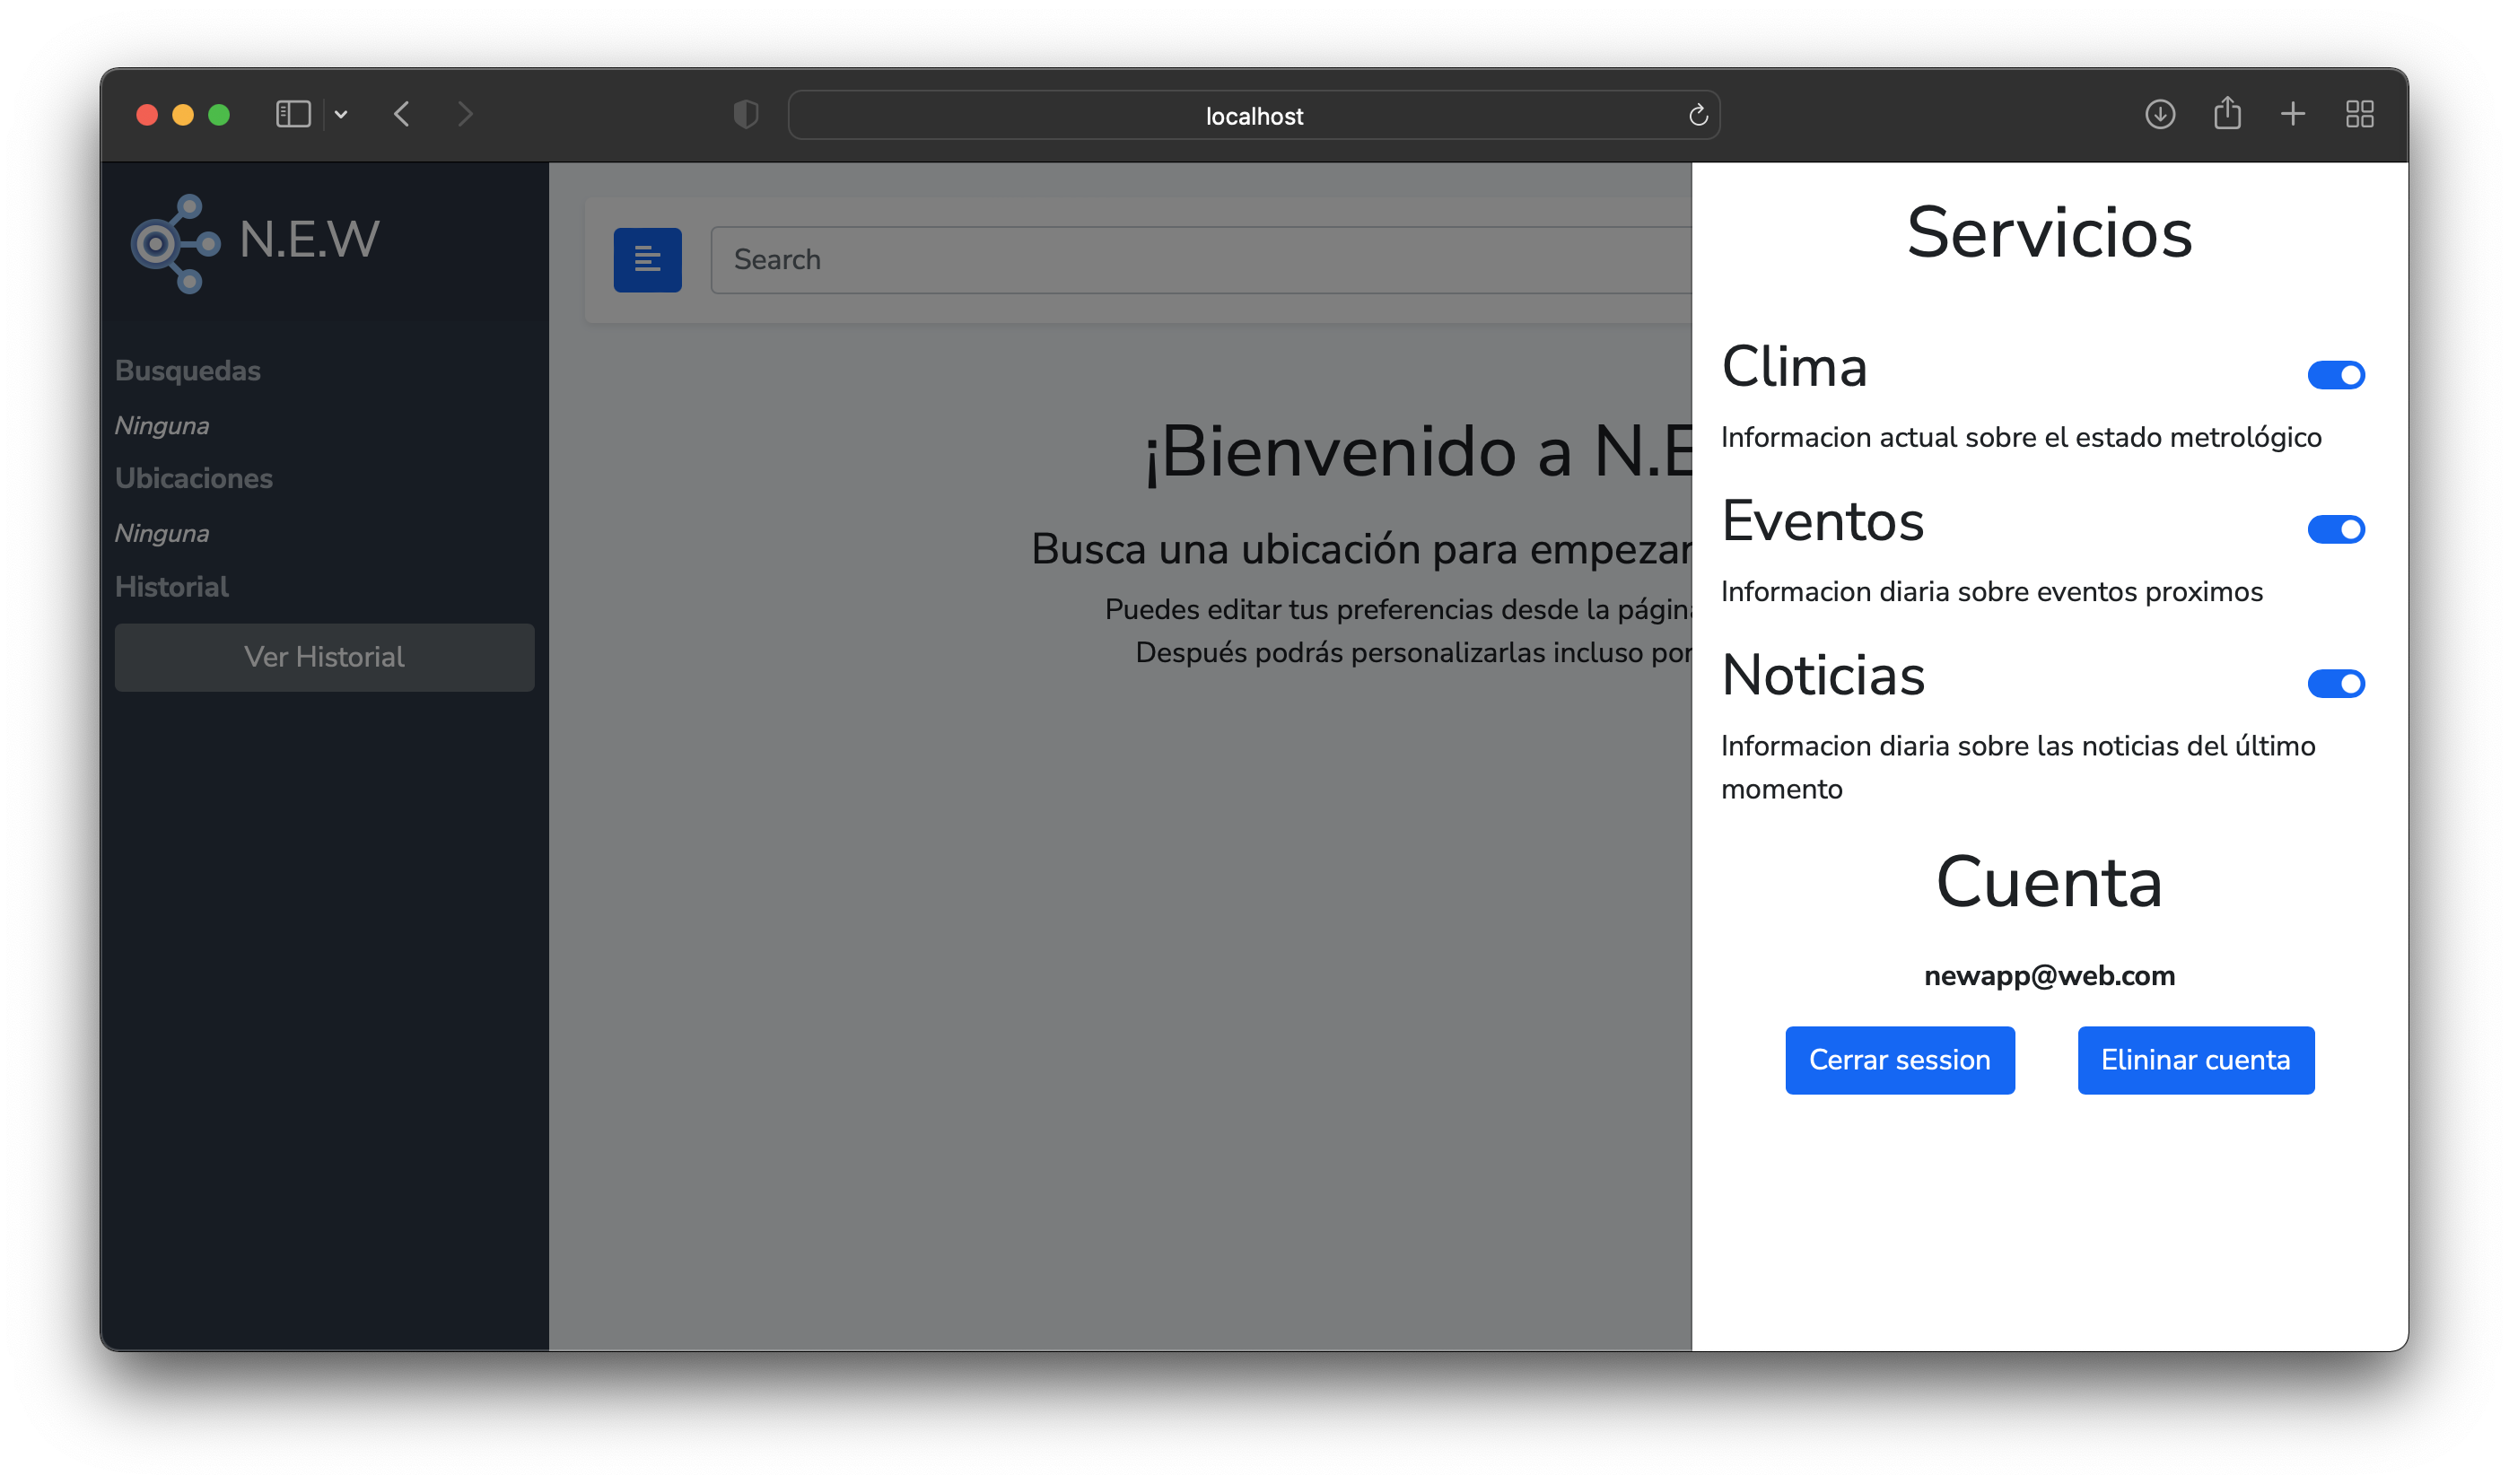
\includegraphics[scale=0.342]{images/final3.png}
                                    \end{center}
                                \end{figure}

                                Llegados a este punto, podemos utilizar la aplicación directamente. Introducimos en el campo de búsqueda superior \textit{Barcelona}, probablemente a medida que vayamos itroduciendo el texto, la aplicación nos sugiera una ubicación. Como información extra, se dan también las coordenadas de la ubicación.\\


                                \begin{figure}[H]
                                    \begin{center}
                                    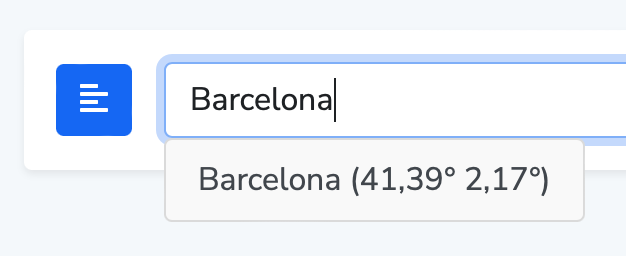
\includegraphics[scale=0.50]{images/finaltextoautocompletado.png}
                                    \end{center}
                                \end{figure}

                                Une vez elegimos una ubicación, el servidor cargará el resto de información y se mostrará el clima, eventos y noticias relacionados con dicha ubicación:


                                \begin{figure}[H]
                                    \begin{center}
                                        \hspace*{-9mm}
                                    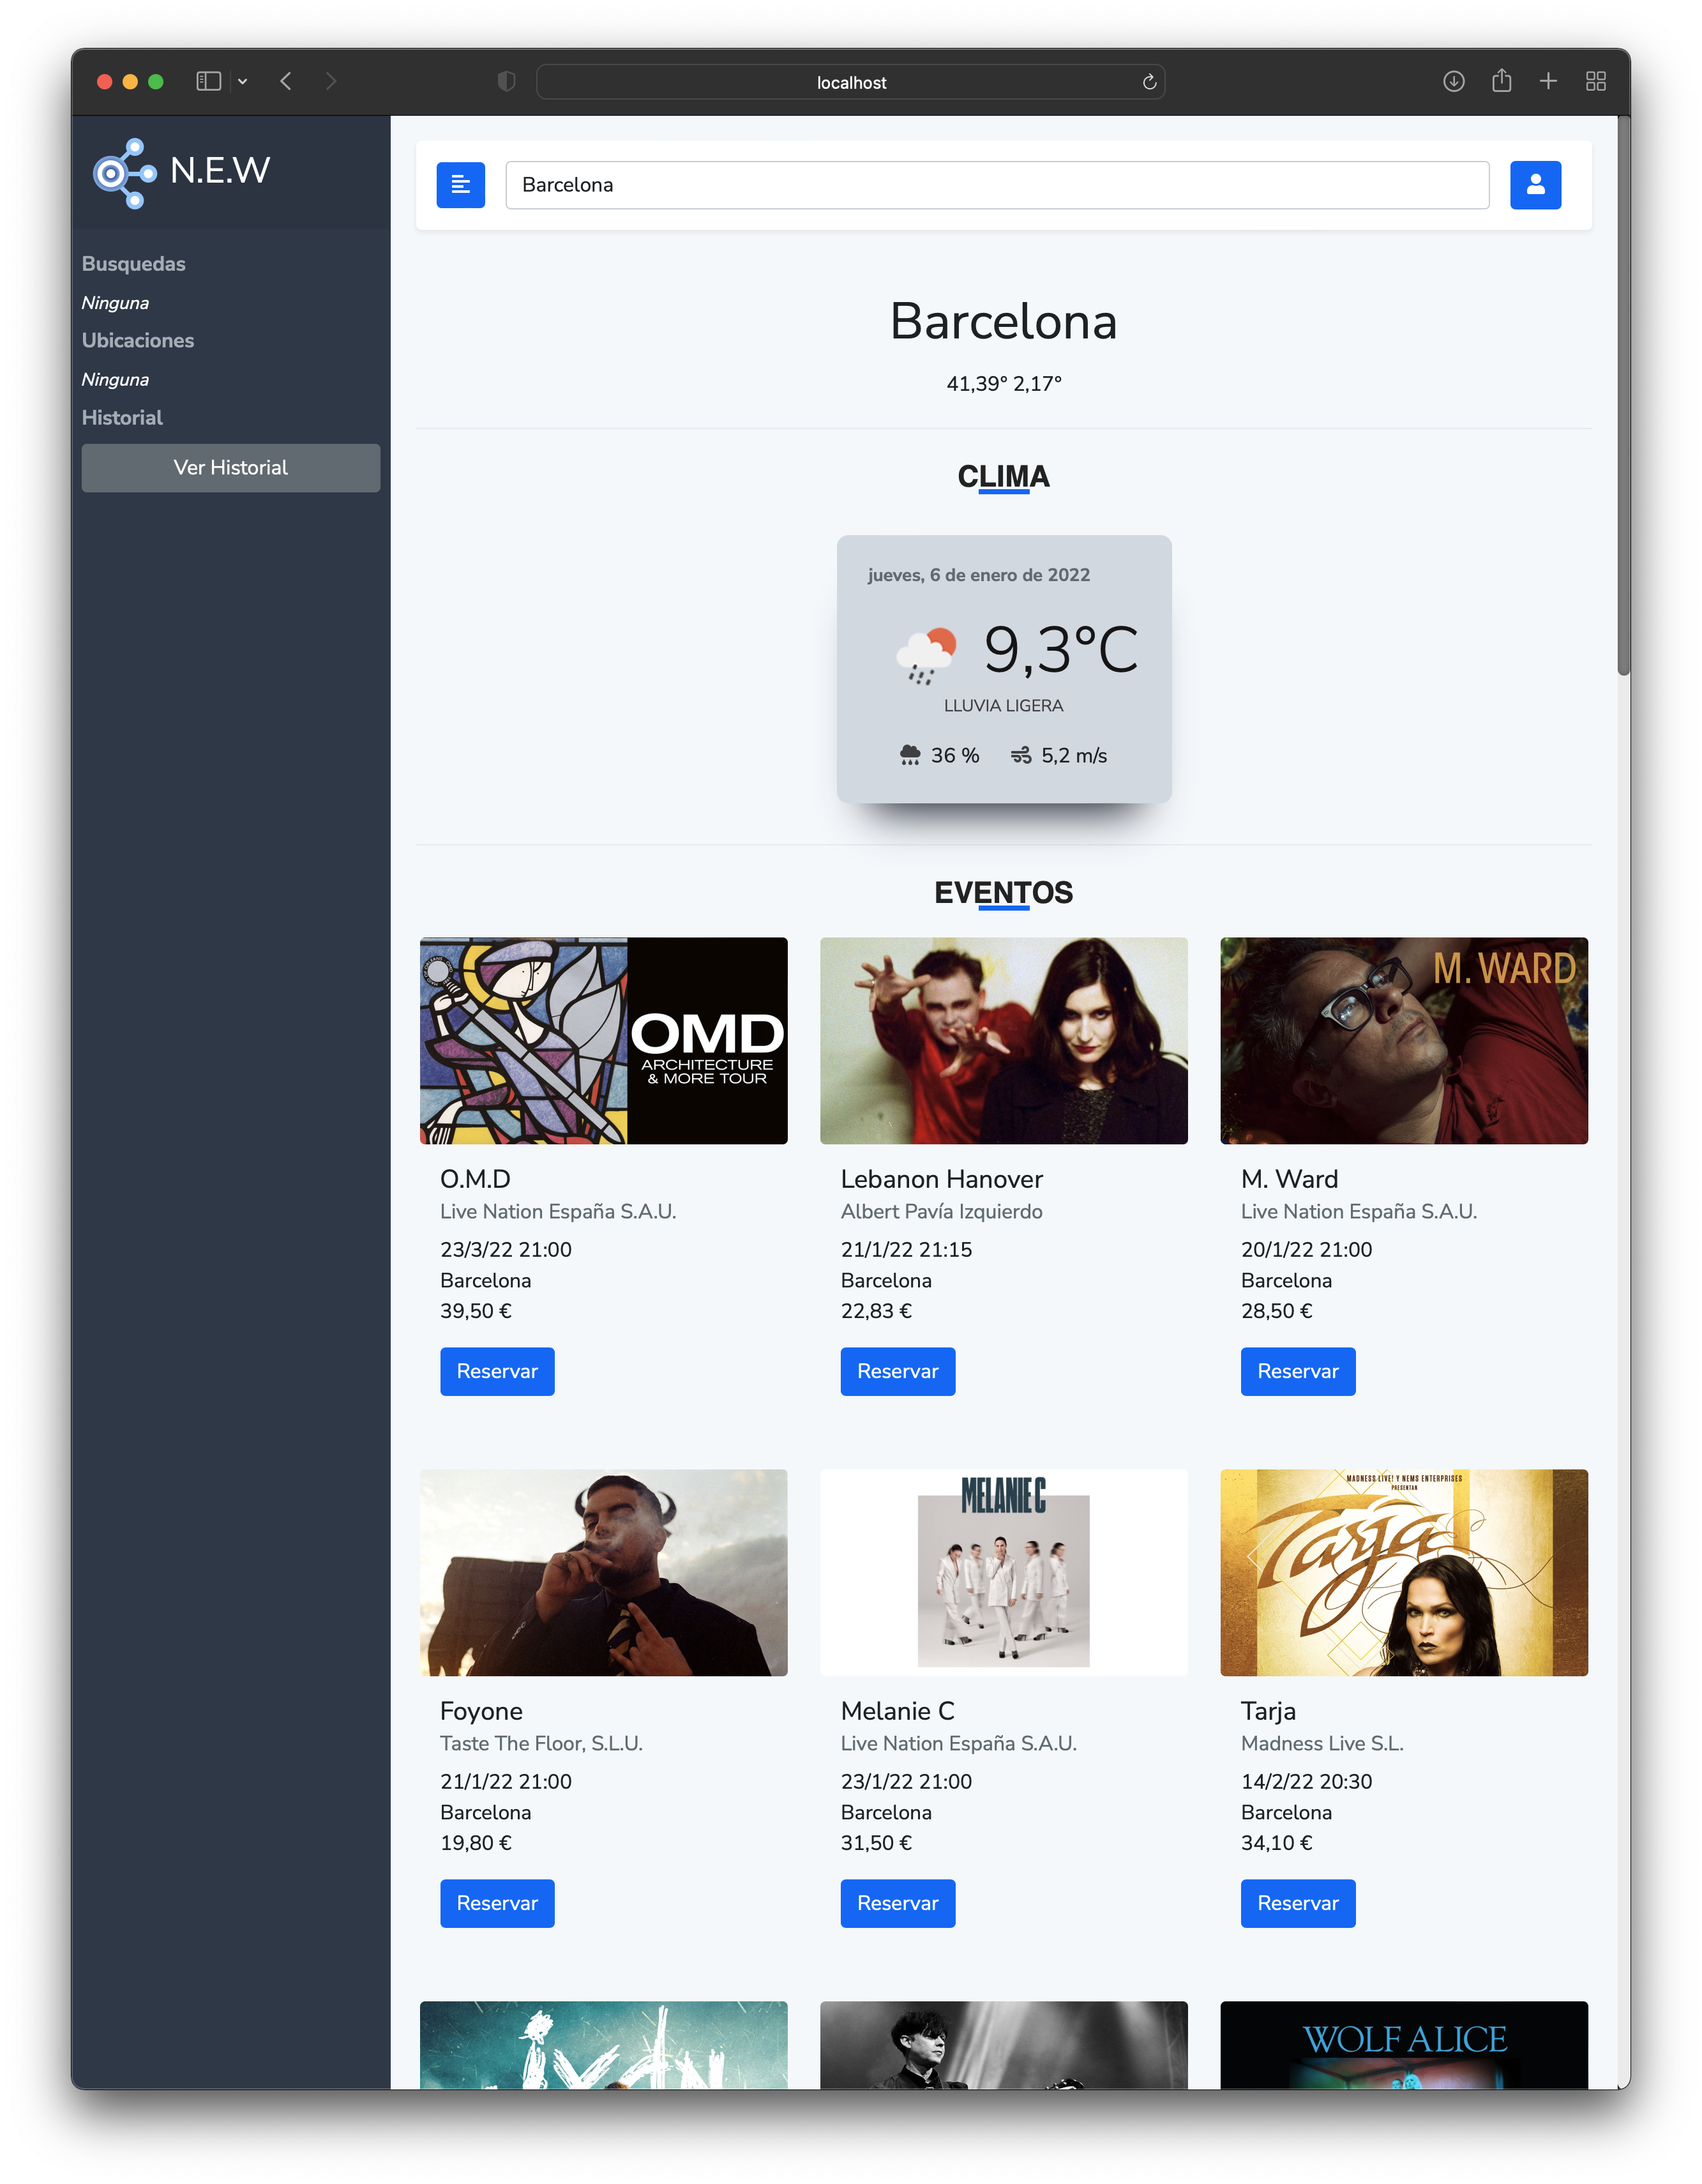
\includegraphics[scale=0.37]{images/final4.png}
                                    \end{center}
                                \end{figure}

                                \newpage

                                Podemos ver, que cada uno de los enlaces de '\textit{Reservar}' o '\textit{Seguir leyendo}' lleva a un link externo por parte del proveedor de la api. Tal y como se puede observar en la imágen siguiente con el link de una de las noticias.

                                \vspace*{-3mm}
                                \begin{figure}[H]
                                    \begin{center}
                                        \hspace*{-12mm}
                                    \includegraphics[scale=0.335]{images/final5.png}
                                    \end{center}
                                \end{figure}

                                También, si lo deseamos, podemos guardar una ubicación como favorita, o incluso crearle un alias.

                                \paragraph{Responsividad y diseño en dispositivos móviles}

                                En una página web la responsividad o capacidad de respuesta es sumamente importante, porque es el parámetro que decide como se va a ver la página web en diferentes layouts, y la capacidad que va a tener de adaptarse y reordenar su información dependiendo de un input dado.\\

                                A continuación se puede observar cómo la página principal del proyecto es capaz de reordenar sus iconos y tarjetas de información para adaptarse al ancho disponible del navegador:


                                \begin{figure}[H]  
                                    \begin{center}
                                    \hspace*{-12mm} 
                                    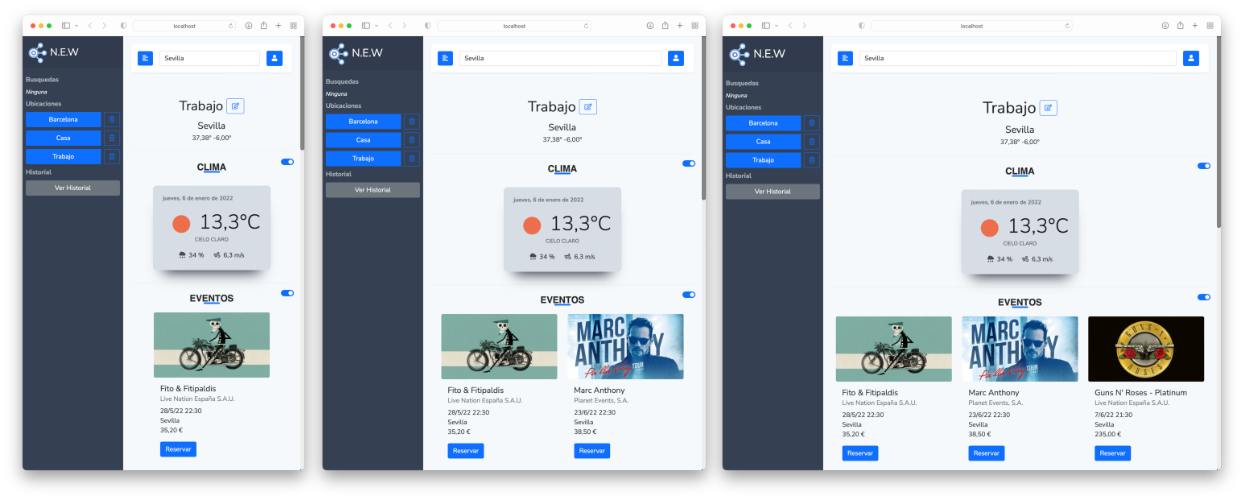
\includegraphics[scale=0.4]{images/Responsivo.png}
                                    \end{center}
                                    \caption{Ejemplo de responsividad en la página web}
                                \end{figure}

                                En los últimos años, con el uso más frecuente de dispositivo móviles, es bastante más usual ver como la mayoría se sitios web, o bien cuentan con una versión movil, o estan pdogramados para que sean responsivos y por lo tanto se adapten de forma automática a estos layouts más reducidos. Cada día es más frecuente el uso de dispositivos móviles, por lo que una web que ofrezca responsividad de forma adecuada, es de crucial importancia en IT.\\

                                A continuación, una comparativa de como se ve la página web en dos dispositivos móviles bastante diferentes, en un iPhone 13 Pro Max y un iPad Pro 12,9 de 2021. Pese a que la resolución del iPhone sea bastante elevada, el tamaño de la pantalla en comparación al del iPad Pro es bastante pequeña, por lo que los elementos en el navegador deben reordenarse (hacen uso de la responsividad) para que sean cómodos de leer por parte del usuario.

                                \newpage

                                Los dispositivos se muestran a escala, respetando las proporciones originales.


                                \begin{figure}[H]
                                    \begin{center}
                                        \hspace*{-3mm} 
                                    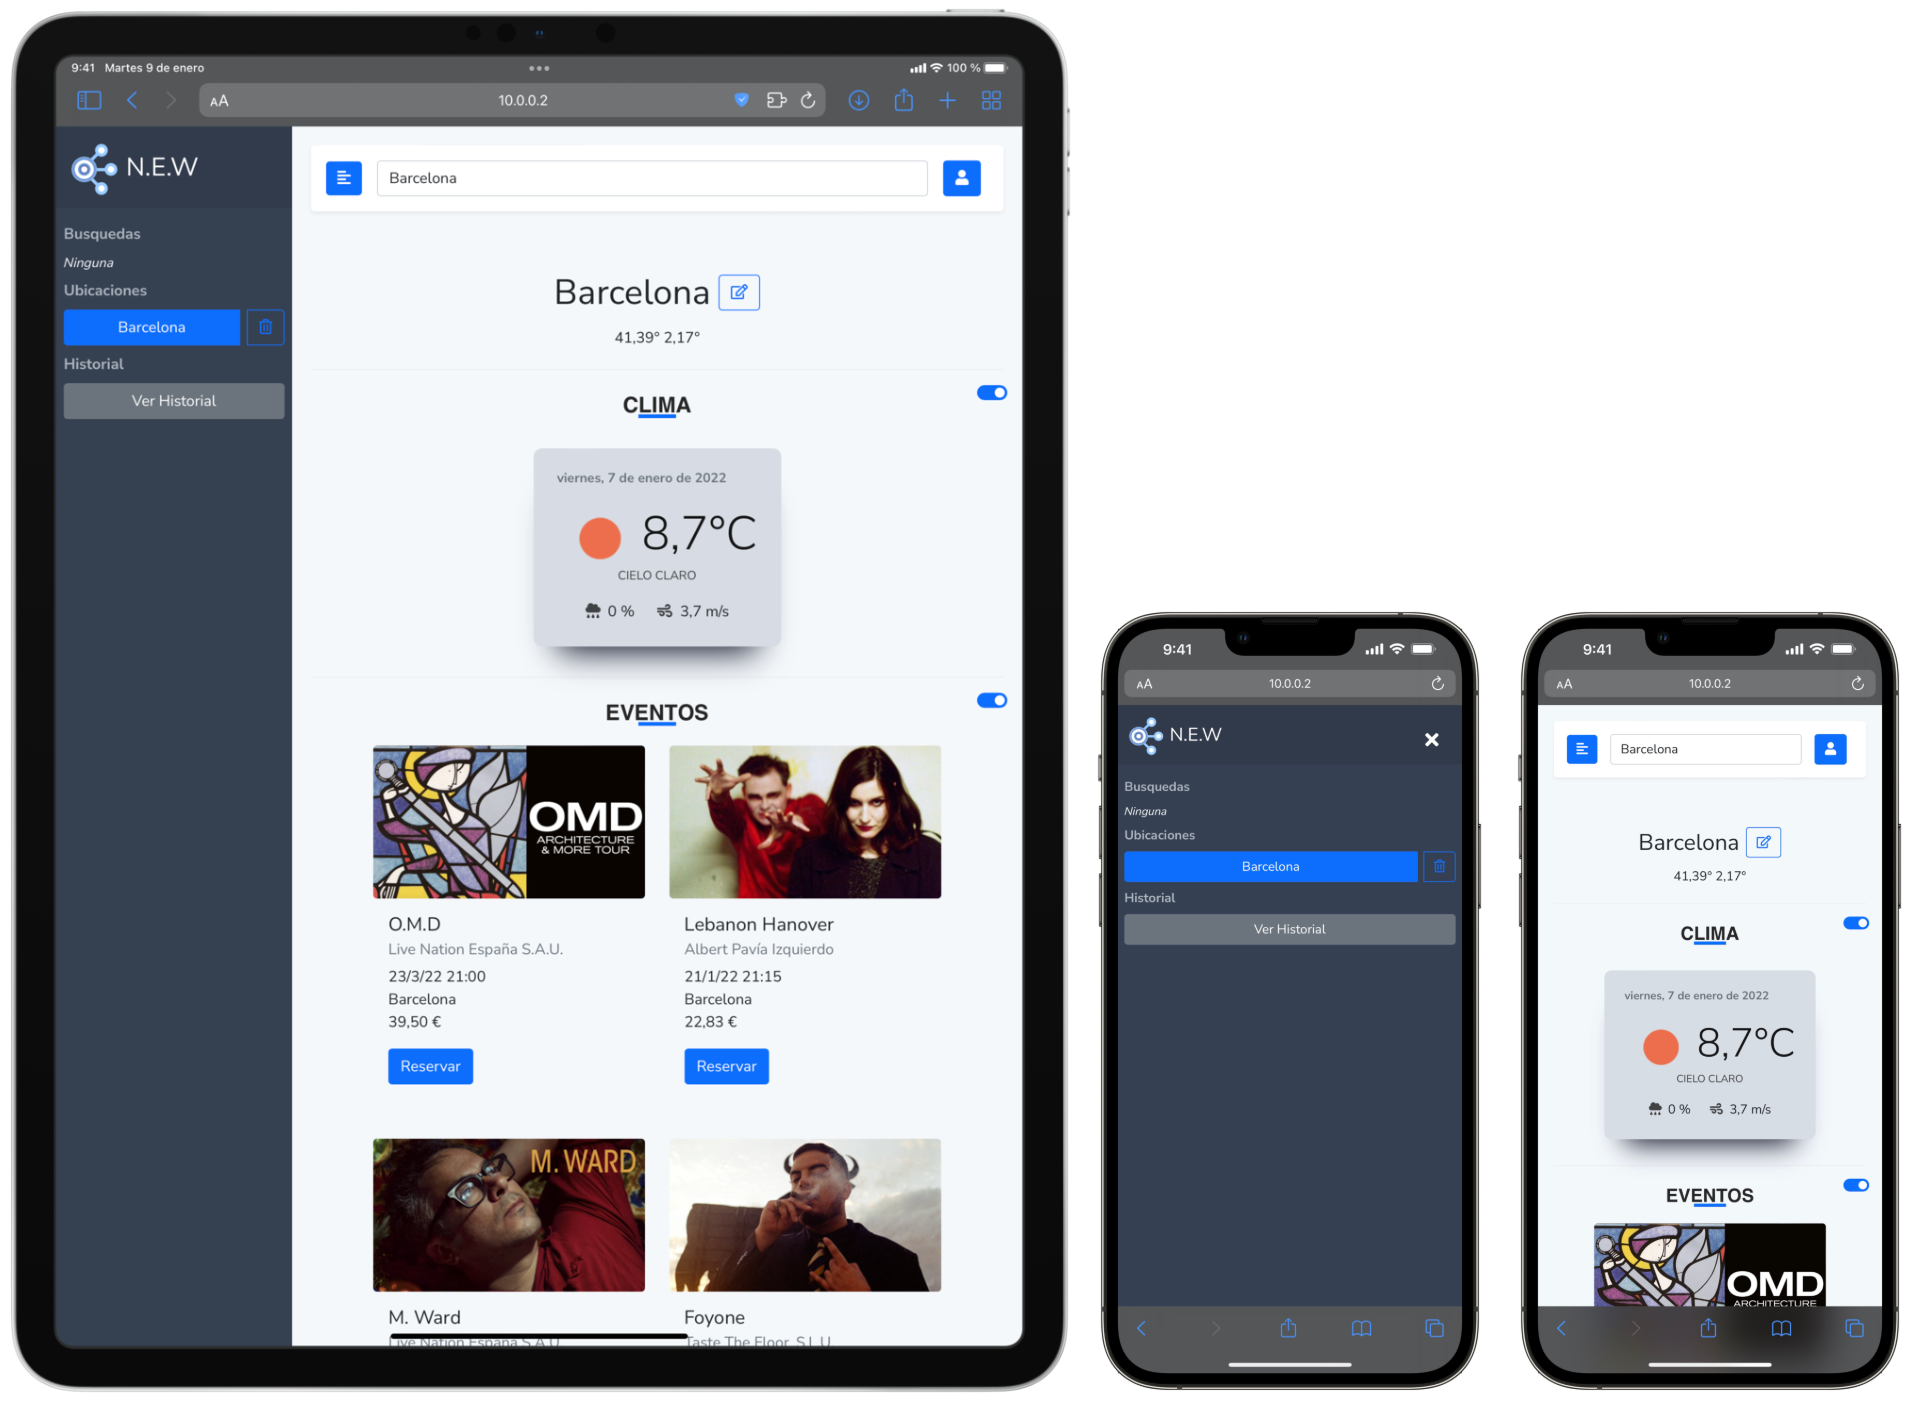
\includegraphics[scale=0.24]{images/ipadiphonecomparacion.png}
                                    \end{center}
                                    \caption{Comparación de responsividad: iPad Pro y iPhone 13 Pro Max}
                                \end{figure}



                                Tal y como se puede apreciar, lo que en un simple pantallazo en un navegador con mayor dimensión es suficiente, en dispositivos móviles, tenemos diferentes \textit{layouts}, en este caso, uno para la pantalla principal y otro para los ajustes de ubicaciones.\\

                                Haciendo uso de la responsividad, a continuación un pequeño \textit{sneak peak} de como se ve la aplicación con un dispositivo movil.\\
                                
                                El uso que le hemos dado para esta pequeña demostración es sencillo: crear una cuenta de usuario, introducir un total de 3 ubicaciones, y marcarlas todas como favoritas; cambiar el nombre de una de ellas, y finalmente consultar un par de enlaces, uno de entradas para un concierto y otro de una noticia de actualidad\footnote{Nótese como los enlaces que se proporcionan, abren directamente una pestaña nueva a la noticia o evento que queremos ver.}.

                                \newpage

                                \begin{figure}[H]
                                    \begin{center}
                                        \hspace*{-10mm} 
                                    \includegraphics[scale=0.15]{images/telefonos1.png}
                                    \end{center}
                                \end{figure}

                                \newpage

                                \begin{figure}[H]
                                    \begin{center}
                                        \hspace*{-10mm} 
                                    \includegraphics[scale=0.15]{images/telefonos2.png}
                                    \end{center}
                                \end{figure}

                                \newpage



            

\end{document}